\documentclass[12pt,twoside]{article}

\usepackage{amssymb}
\usepackage{amsmath}
\usepackage{amsthm}
\usepackage{graphicx}
\usepackage{latexsym}
\usepackage{times,url}
\usepackage{cprotect}
\usepackage{listings}
\usepackage{graphicx}
\usepackage[table]{xcolor}
\usepackage[letterpaper]{geometry}
\usepackage{tikz-qtree}
\usepackage{enumerate}
\usepackage{enumitem}
\usepackage{minted}
\usemintedstyle{colorful}

\newcommand{\profs}{Instructor: Tatsunori Hashimoto}
\newcommand{\subj}{CS336}
\newcommand{\ttt}[1]{{\tt\small #1}}

\definecolor{dkgreen}{rgb}{0,0.6,0}
\definecolor{dkblue}{rgb}{.2,.2,1}
\definecolor{gray}{rgb}{0.5,0.5,0.5}
\definecolor{mauve}{rgb}{0.58,0,0.82}

\lstset{
  language=Python,
  aboveskip=1pc,
  belowskip=1pc,
  basicstyle={\footnotesize\ttfamily},
  numbers=left,
  showstringspaces=false,
  numberstyle={\tiny\color{gray}\ttfamily},
  keywordstyle={\color{dkblue}\ttfamily},
  commentstyle={\color{dkgreen}\ttfamily},
  stringstyle={\color{mauve}\ttfamily},
}

% \lstset{
%   language=Python,
%   aboveskip=1pc,
%   belowskip=1pc,
%   basicstyle={\bf\color{white}\ttfamily},
%   numbers=left,
%   showstringspaces=false,
%   numberstyle={\bf\small\color{lightgray}\ttfamily},
%   keywordstyle={\bf\color{cyan}\ttfamily},
%   commentstyle={\bf\color{green}\ttfamily},
%   stringstyle={\bf\color{mauve}\ttfamily},
% }

\tikzset{
  % every node/.style={minimum width=2em,draw,circle},
  % level 1/.style={sibling distance=2cm},
  level distance=1cm,
  edge from parent/.style=
  {draw,edge from parent path={(\tikzparentnode) -- (\tikzchildnode)}},
}
\usetikzlibrary{shapes}

\newif\ifHideSolutions
\newcommand{\solution}[1]{\color{dkgreen}\textbf{Solution: }#1\color{black}}
\newcommand{\commonmistakes}[1]{{\color{dkblue}\textbf{Common Mistakes: }#1}}
\newcommand{\rubric}[1]{\color{dkgreen}{\bf Rubric:} #1\color{black}}

% \HideSolutionsfalse
% \ifHideSolutions
%   \renewcommand{\solution}[1]{}
%   \renewcommand{\rubric}[1]{}
% \fi

\newlength{\toppush}
\setlength{\toppush}{2\headheight}
\addtolength{\toppush}{\headsep}

\newcommand{\htitle}[2]{\noindent\vspace*{-\toppush}\newline\parbox{\textwidth}
{\textit{Language Modeling: CS336}\hfill\name\newline
Stanford Online \hfill #2\newline
\profs\hfill #1 \\[-3.5ex]\newline
\mbox{}\hrulefill\mbox{}}\vspace*{1ex}\mbox{}\newline
\begin{center}{\Large\bf #1}\end{center}}

\newcommand{\handout}[2]{\thispagestyle{empty}
 \markboth{#1}{#1}
 \pagestyle{myheadings}\htitle{#1}{#2}}

\newcommand{\lecture}[3]{\thispagestyle{empty}
 \markboth{Lecture #1: #2}{Lecture #1: #2}
 \pagestyle{myheadings}\htitle{Lecture #1: #2}{#3}}

\newcommand{\htitlewithouttitle}[2]{\noindent\vspace*{-\toppush}\newline\parbox{6.5in}
{\textit{Language Modeling}\hfill#2\newline
Stanford Online \hfill 18.701\newline
\profs\hfill Handout #1\vspace*{-.5ex}\newline
\mbox{}\hrulefill\mbox{}}\vspace*{1ex}\mbox{}\newline}

\newcommand{\handoutwithouttitle}[2]{\thispagestyle{empty}
 \markboth{Handout \protect\ref{#1}}{Handout \protect\ref{#1}}
 \pagestyle{myheadings}\htitlewithouttitle{\protect\ref{#1}}{#2}}

\newcommand{\exam}[2]{% parameters: exam name, date
 \thispagestyle{empty}
 \markboth{\hspace{1cm}\subj\ #1\hspace{1in}Name\hrulefill\ \ }%
          {\subj\ #1\hspace{1in}Name\hrulefill\ \ }
 \pagestyle{myheadings}\examtitle{#1}{#2}
 \renewcommand{\theproblem}{Problem \arabic{problemnum}}
}
\newcommand{\examsolutions}[3]{% parameters: handout, exam name, date
 \thispagestyle{empty}
 \markboth{Handout \protect\ref{#1}: #2}{Handout \protect\ref{#1}: #2}
% \pagestyle{myheadings}\htitle{\protect\ref{#1}}{#2}{#3}
 \pagestyle{myheadings}\examsolutionstitle{\protect\ref{#1}} {#2}{#3}
 \renewcommand{\theproblem}{Problem \arabic{problemnum}}
}
\newcommand{\examsolutionstitle}[3]{\noindent\vspace*{-\toppush}\newline\parbox{6.5in}
{\textit{Language Modeling}\hfill#3\newline
Stanford Online \hfill CS336\newline
%Singapore-MIT Alliance \hfill SMA5503\newline
\profs\hfill Handout #1\vspace*{-.5ex}\newline
\mbox{}\hrulefill\mbox{}}\vspace*{1ex}\mbox{}\newline
\begin{center}{\Large\bf #2}\end{center}}

\newcommand{\takehomeexam}[2]{% parameters: exam name, date
 \thispagestyle{empty}
 \markboth{\subj\ #1\hfill}{\subj\ #1\hfill}
 \pagestyle{myheadings}\examtitle{#1}{#2}
 \renewcommand{\theproblem}{Problem \arabic{problemnum}}
}

\makeatletter
\newcommand{\exambooklet}[2]{% parameters: exam name, date
 \thispagestyle{empty}
 \markboth{\subj\ #1}{\subj\ #1}
 \pagestyle{myheadings}\examtitle{#1}{#2}
 \renewcommand{\theproblem}{Problem \arabic{problemnum}}
 \renewcommand{\problem}{\newpage
 \item \let\@currentlabel=\theproblem
 \markboth{\subj\ #1, \theproblem}{\subj\ #1, \theproblem}}
}
\makeatother


\newcommand{\examtitle}[2]{\noindent\vspace*{-\toppush}\newline\parbox{6.5in}
{\textit{Language Modeling}\hfill#2\newline
Stanford Online \hfill CS336 Spring 2026\newline
%Singapore-MIT Alliance \hfill SMA5503\newline
\profs\hfill #1\vspace*{-.5ex}\newline
\mbox{}\hrulefill\mbox{}}\vspace*{1ex}\mbox{}\newline
\begin{center}{\Large\bf #1}\end{center}}

\newcommand{\grader}[1]{\hspace{1cm}\textsf{\textbf{#1}}\hspace{1cm}}

\newcommand{\points}[1]{[#1 points]\ }
\newcommand{\parts}[1]
{
  \ifnum#1=1
  (1 part)
  \else
  (#1 parts)
  \fi
  \ 
}

\newcommand{\bparts}{\begin{problemparts}}
\newcommand{\eparts}{\end{problemparts}}
\newcommand{\ppart}{\problempart}

%\newcommand{\lg} {lg\ }

\setlength{\oddsidemargin}{0pt}
\setlength{\evensidemargin}{0pt}
\setlength{\textwidth}{6.5in}
\setlength{\topmargin}{0in}
\setlength{\textheight}{8.5in}


\newcommand{\Spawn}{{\bf spawn} }
\newcommand{\Sync}{{\bf sync}}

\renewcommand{\cases}[1]{\left\{ \begin{array}{ll}#1\end{array}\right.}
\newcommand{\cif}[1]{\mbox{if $#1$}}
\newcommand{\cwhen}[1]{\mbox{when $#1$}}

\newcounter{problemnum}
\newcommand{\theproblem}{Problem \theproblemsetnum-\arabic{problemnum}}
\newenvironment{problems}{
        \begin{list}{{\bf \theproblem. \hspace*{0.5em}}}
        {\setlength{\leftmargin}{0em}
         \setlength{\rightmargin}{0em}
         \setlength{\labelwidth}{0em}
         \setlength{\labelsep}{0em}
         \usecounter{problemnum}}}{\end{list}}
\makeatletter
\newcommand{\problem}[1][{}]{\item \let\@currentlabel=\theproblem \textbf{#1}}
\makeatother

\newcounter{problempartnum}[problemnum]
\newenvironment{problemparts}{
        \begin{list}{{\bf (\alph{problempartnum})}}
        {\setlength{\leftmargin}{2.5em}
         \setlength{\rightmargin}{2.5em}
         \setlength{\labelsep}{0.5em}}}{\end{list}}
\newcommand{\problempart}{\addtocounter{problempartnum}{1}\item}

\newenvironment{truefalseproblemparts}{
        \begin{list}{{\bf (\alph{problempartnum})\ \ \ T\ \ F\hfil}}
        {\setlength{\leftmargin}{4.5em}
         \setlength{\rightmargin}{2.5em}
         \setlength{\labelsep}{0.5em}
         \setlength{\labelwidth}{4.5em}}}{\end{list}}

\newcounter{exercisenum}
\newcommand{\theexercise}{Exercise \theproblemsetnum-\arabic{exercisenum}}
\newenvironment{exercises}{
        \begin{list}{{\bf \theexercise. \hspace*{0.5em}}}
        {\setlength{\leftmargin}{0em}
         \setlength{\rightmargin}{0em}
         \setlength{\labelwidth}{0em}
         \setlength{\labelsep}{0em}
        \usecounter{exercisenum}}}{\end{list}}
\makeatletter
\newcommand{\exercise}{\item \let\@currentlabel=\theexercise}
\makeatother

\newcounter{exercisepartnum}[exercisenum]
%\newcommand{\problem}[1]{\medskip\mbox{}\newline\noindent{\bf Problem #1.}\hspace*{1em}}
%\newcommand{\exercise}[1]{\medskip\mbox{}\newline\noindent{\bf Exercise #1.}\hspace*{1em}}

\newenvironment{exerciseparts}{
        \begin{list}{{\bf (\alph{exercisepartnum})}}
        {\setlength{\leftmargin}{2.5em}
         \setlength{\rightmargin}{2.5em}
         \setlength{\labelsep}{0.5em}}}{\end{list}}
\newcommand{\exercisepart}{\addtocounter{exercisepartnum}{1}\item}


% Macros to make captions print with small type and 'Figure xx' in bold.
\makeatletter
\def\fnum@figure{{\bf Figure \thefigure}}
\def\fnum@table{{\bf Table \thetable}}
\let\@mycaption\caption
%\long\def\@mycaption#1[#2]#3{\addcontentsline{\csname
%  ext@#1\endcsname}{#1}{\protect\numberline{\csname 
%  the#1\endcsname}{\ignorespaces #2}}\par
%  \begingroup
%    \@parboxrestore
%    \small
%    \@makecaption{\csname fnum@#1\endcsname}{\ignorespaces #3}\par
%  \endgroup}
%\def\mycaption{\refstepcounter\@captype \@dblarg{\@mycaption\@captype}}
%\makeatother
\let\mycaption\caption
%\newcommand{\figcaption}[1]{\mycaption[]{#1}}

\newcounter{totalcaptions}
\newcounter{totalart}

\newcommand{\figcaption}[1]{\addtocounter{totalcaptions}{1}\caption[]{#1}}

% \psfigures determines what to do for figures:
%       0 means just leave vertical space
%       1 means put a vertical rule and the figure name
%       2 means insert the PostScript version of the figure
%       3 means put the figure name flush left or right
\newcommand{\psfigures}{0}
\newcommand{\spacefigures}{\renewcommand{\psfigures}{0}}
\newcommand{\rulefigures}{\renewcommand{\psfigures}{1}}
\newcommand{\macfigures}{\renewcommand{\psfigures}{2}}
\newcommand{\namefigures}{\renewcommand{\psfigures}{3}}

\newcommand{\figpart}[1]{{\bf (#1)}\nolinebreak[2]\relax}
\newcommand{\figparts}[2]{{\bf (#1)--(#2)}\nolinebreak[2]\relax}


\macfigures     % STATE

% When calling \figspace, make sure to leave a blank line afterward!!
% \widefigspace is for figures that are more than 28pc wide.
\newlength{\halffigspace} \newlength{\wholefigspace}
\newlength{\figruleheight} \newlength{\figgap}
\newcommand{\setfiglengths}{\ifnum\psfigures=1\setlength{\figruleheight}{\hruleheight}\setlength{\figgap}{1em}\else\setlength{\figruleheight}{0pt}\setlength{\figgap}{0em}\fi}
\newcommand{\figspace}[2]{\ifnum\psfigures=0\leavefigspace{#1}\else%
\setfiglengths%
\setlength{\wholefigspace}{#1}\setlength{\halffigspace}{.5\wholefigspace}%
\rule[-\halffigspace]{\figruleheight}{\wholefigspace}\hspace{\figgap}#2\fi}
\newlength{\widefigspacewidth}
% Make \widefigspace put the figure flush right on the text page.
\newcommand{\widefigspace}[2]{
\ifnum\psfigures=0\leavefigspace{#1}\else%
\setfiglengths%
\setlength{\widefigspacewidth}{28pc}%
\addtolength{\widefigspacewidth}{-\figruleheight}%
\setlength{\wholefigspace}{#1}\setlength{\halffigspace}{.5\wholefigspace}%
\makebox[\widefigspacewidth][r]{#2\hspace{\figgap}}\rule[-\halffigspace]{\figruleheight}{\wholefigspace}\fi}
\newcommand{\leavefigspace}[1]{\setlength{\wholefigspace}{#1}\setlength{\halffigspace}{.5\wholefigspace}\rule[-\halffigspace]{0em}{\wholefigspace}}

% Commands for including figures with macpsfig.
% To use these commands, documentstyle ``macpsfig'' must be specified.
\newlength{\macfigfill}
\makeatother
\newlength{\bbx}
\newlength{\bby}
\newcommand{\macfigure}[5]{\addtocounter{totalart}{1}
\ifnum\psfigures=2%
\setlength{\bbx}{#2}\addtolength{\bbx}{#4}%
\setlength{\bby}{#3}\addtolength{\bby}{#5}%
\begin{flushleft}
\ifdim#4>28pc\setlength{\macfigfill}{#4}\addtolength{\macfigfill}{-28pc}\hspace*{-\macfigfill}\fi%
\mbox{\psfig{figure=./#1.ps,%
bbllx=#2,bblly=#3,bburx=\bbx,bbury=\bby}}
\end{flushleft}%
\else\ifdim#4>28pc\widefigspace{#5}{#1}\else\figspace{#5}{#1}\fi\fi}
\makeatletter

\newlength{\savearraycolsep}
\newcommand{\narrowarray}[1]{\setlength{\savearraycolsep}{\arraycolsep}\setlength{\arraycolsep}{#1\arraycolsep}}
\newcommand{\normalarray}{\setlength{\arraycolsep}{\savearraycolsep}}

\newcommand{\hint}{{\bf Hint:\ }}

% Macros from /th/u/clr/mac.tex

\newcommand{\set}[1]{\left\{ #1 \right\}}
\newcommand{\abs}[1]{\left| #1\right|}
\newcommand{\card}[1]{\left| #1\right|}
\newcommand{\floor}[1]{\left\lfloor #1 \right\rfloor}
\newcommand{\ceil}[1]{\left\lceil #1 \right\rceil}
\newcommand{\ang}[1]{\ifmmode{\left\langle #1 \right\rangle}
   \else{$\left\langle${#1}$\right\rangle$}\fi}
        % the \if allows use outside mathmode,
        % but will swallow following space there!
\newcommand{\paren}[1]{\left( #1 \right)}
\newcommand{\bracket}[1]{\left[ #1 \right]}
\newcommand{\prob}[1]{\Pr\left\{ #1 \right\}}
\newcommand{\Var}{\mathop{\rm Var}\nolimits}
\newcommand{\expect}[1]{{\rm E}\left[ #1 \right]}
\newcommand{\expectsq}[1]{{\rm E}^2\left[ #1 \right]}
\newcommand{\variance}[1]{{\rm Var}\left[ #1 \right]}
\renewcommand{\choose}[2]{{{#1}\atopwithdelims(){#2}}}
\def\pmod#1{\allowbreak\mkern12mu({\rm mod}\,\,#1)}
\newcommand{\matx}[2]{\left(\begin{array}{*{#1}{c}}#2\end{array}\right)}
\newcommand{\Adj}{\mathop{\rm Adj}}

\newtheoremstyle{boldnote}% name of the style
  {\topsep}%          Space above
  {\topsep}%          Space below
  {\itshape}%         Body font
  {}%                 Indent amount
  {\bfseries}%        Theorem head font (Theorem)
  {:}%                Punctuation after theorem head
  {.5em}%             Space after theorem head
  {\thmname{#1}\thmnumber{ #2}\thmnote{ (\bfseries #3)}} % <--- Bolds the note text
\theoremstyle{boldnote}
\newtheorem*{claim}{Claim}
\newtheorem*{theorem}{Theorem}
\newtheorem*{lemma}{Lemma}
\newtheorem*{corollary}{Corollary}
\newtheorem*{fact}{Fact}
\newtheorem*{xample}{Example}
\newtheorem*{definition}{Definition}
\newtheorem*{remark}{Remark}
\newtheorem*{question}{Question}
\newenvironment{example}{\begin{xample}\rm}{\end{xample}}
\newcommand{\proof}{\noindent{\em Proof.}\hspace{1em}}
\def\squarebox#1{\hbox to #1{\hfill\vbox to #1{\vfill}}}
\newcommand{\qedbox}{\vbox{\hrule\hbox{\vrule\squarebox{.667em}\vrule}\hrule}}
\newcommand{\qed}{\nopagebreak\mbox{}\hfill\qedbox\smallskip}
\newcommand{\eqnref}[1]{(\protect\ref{#1})}

%%\newcommand{\twodots}{\mathinner{\ldotp\ldotp}}
\newcommand{\transpose}{^{\mbox{\scriptsize \sf T}}}
\newcommand{\amortized}[1]{\widehat{#1}}

\newcommand{\punt}[1]{}

%%% command for putting definitions into boldface
% New style for defined terms, as of 2/23/88, redefined by THC.
\newcommand{\defn}[1]{{\boldmath\textit{\textbf{#1}}}}
\newcommand{\defi}[1]{{\textit{\textbf{#1\/}}}}

\newcommand{\red}{\leq_{\rm P}}
\newcommand{\lang}[1]{%
\ifmmode\mathord{\mathcode`-="702D\rm#1\mathcode`\-="2200}\else{\rm#1}\fi}

%\newcommand{\ckt}[1]{\ifmmode\mathord{\mathcode`-="702D\sc #1\mathcode`\-="2200}\else$\mathord{\mathcode`-="702D\sc #1\mathcode`\-="2200}$\fi}
\newcommand{\ckt}[1]{\ifmmode \sc #1\else$\sc #1$\fi}

%% Margin notes - use \notesfalse to turn off notes.
\setlength{\marginparwidth}{0.6in}
\reversemarginpar
\newif\ifnotes
\notestrue
\newcommand{\longnote}[1]{
  \ifnotes
    {\medskip\noindent Note: \marginpar[\hfill$\Longrightarrow$]
      {$\Longleftarrow$}{#1}\medskip}
  \fi}
\newcommand{\note}[1]{
  \ifnotes
    {\marginpar{\tiny \raggedright{#1}}}
  \fi}


\newcommand{\reals}{\mathbbm{R}}
\newcommand{\integers}{\mathbbm{Z}}
\newcommand{\naturals}{\mathbbm{N}}
\newcommand{\rationals}{\mathbbm{Q}}
\newcommand{\complex}{\mathbbm{C}}

\newcommand{\oldreals}{{\bf R}}
\newcommand{\oldintegers}{{\bf Z}}
\newcommand{\oldnaturals}{{\bf N}}
\newcommand{\oldrationals}{{\bf Q}}
\newcommand{\oldcomplex}{{\bf C}}

\newcommand{\w}{\omega}                 %% for fft chapter

\newenvironment{closeitemize}{\begin{list}
{$\bullet$}
{\setlength{\itemsep}{-0.2\baselineskip}
\setlength{\topsep}{0.2\baselineskip}
\setlength{\parskip}{0pt}}}
{\end{list}}

% These are necessary within a {problems} environment in order to restore
% the default separation between bullets and items.
\newenvironment{normalitemize}{\setlength{\labelsep}{0.5em}\begin{itemize}}
                              {\end{itemize}}
\newenvironment{normalenumerate}{\setlength{\labelsep}{0.5em}\begin{enumerate}}
                                {\end{enumerate}}

%\def\eqref#1{Equation~(\ref{eq:#1})}
%\newcommand{\eqref}[1]{Equation (\ref{eq:#1})}
\newcommand{\eqreftwo}[2]{Equations (\ref{eq:#1}) and~(\ref{eq:#2})}
\newcommand{\ineqref}[1]{Inequality~(\ref{ineq:#1})}
\newcommand{\ineqreftwo}[2]{Inequalities (\ref{ineq:#1}) and~(\ref{ineq:#2})}

\newcommand{\figref}[1]{Figure~\ref{fig:#1}}
\newcommand{\figreftwo}[2]{Figures \ref{fig:#1} and~\ref{fig:#2}}

\newcommand{\liref}[1]{line~\ref{li:#1}}
\newcommand{\Liref}[1]{Line~\ref{li:#1}}
\newcommand{\lirefs}[2]{lines \ref{li:#1}--\ref{li:#2}}
\newcommand{\Lirefs}[2]{Lines \ref{li:#1}--\ref{li:#2}}
\newcommand{\lireftwo}[2]{lines \ref{li:#1} and~\ref{li:#2}}
\newcommand{\lirefthree}[3]{lines \ref{li:#1}, \ref{li:#2}, and~\ref{li:#3}}

\newcommand{\lemlabel}[1]{\label{lem:#1}}
\newcommand{\lemref}[1]{Lemma~\ref{lem:#1}} 

\newcommand{\exref}[1]{Exercise~\ref{ex:#1}}

\newcommand{\handref}[1]{Handout~\ref{#1}}

\newcommand{\defref}[1]{Definition~\ref{def:#1}}

% (1997.8.16: Victor Luchangco)
% Modified \hlabel to only get date and to use handouts counter for number.
%   New \handout and \handoutwithouttitle commands in newmac.tex use this.
%   The date is referenced by <label>-date.
%   (Retained old definition as \hlabelold.)
%   Defined \hforcelabel to use an argument instead of the handouts counter.

\newcounter{handouts}
\setcounter{handouts}{0}

\newcommand{\hlabel}[2]{%
\stepcounter{handouts}
{\edef\next{\write\@auxout{\string\newlabel{#1}{{\arabic{handouts}}{0}}}}\next}
\write\@auxout{\string\newlabel{#1-date}{{#2}{0}}}
}

\newcommand{\hforcelabel}[3]{%          Does not step handouts counter.
\write\@auxout{\string\newlabel{#1}{{#2}{0}}}
\write\@auxout{\string\newlabel{#1-date}{{#3}{0}}}}


% less ugly underscore
% --juang, 2008 oct 05
\renewcommand{\_}{\vrule height 0 pt depth 0.4 pt width 0.5 em \,}

% multiline framed box (will always extend to the far right edge; for a short single line, use \fbox directly)
% --zabel, fall 2018
\newcommand\framepar[1]{\fbox{\begin{minipage}{\linewidth}#1\end{minipage}}}
\usepackage{float} % needed for [H] placement (harmless if already loaded in macros)
\newcommand{\thelecturenum}{11}

\title{CS336 Lecture 11}

\begin{document}

\handout{Lecture \thelecturenum: Limits of Scaling (and Optimization)}

\setlength{\parindent}{0pt}

\subsection*{Scaling in Practice}

\begin{center}
    What are the best practices for scaling and hparam tuning LMs?
\end{center}

\begin{itemize}
    \item Does Chinchilla's approach to scaling actually work?
    \item Can we save compute when training and fitting these things?
    \item Should we be picking particular architectures / parameterizations to scale nicely?
\end{itemize}

\begin{center}
    The newest model we talked about with scaling details - 2022
\end{center}

\begin{figure}[hpbt]
    \centering
    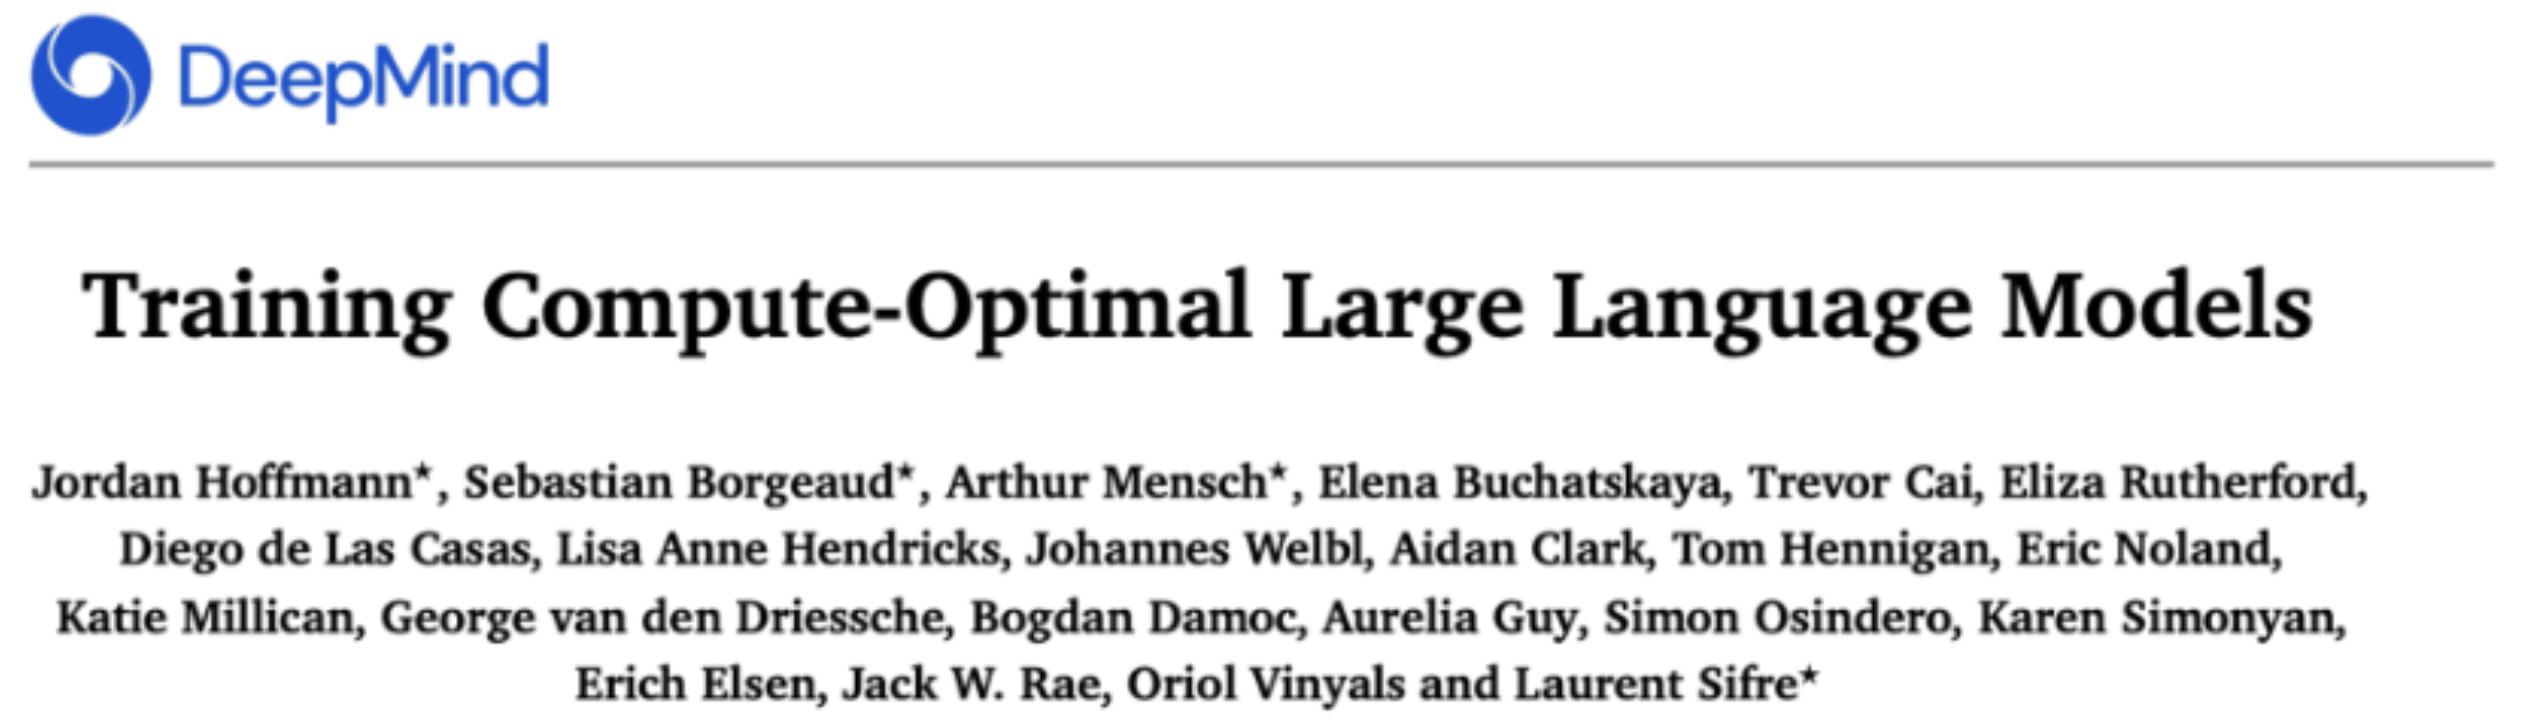
\includegraphics[width=1\linewidth]{chinchilla.png}
\end{figure}

\begin{center}
    What about more recently?
\end{center}

\begin{figure}[hpbt]
    \centering
    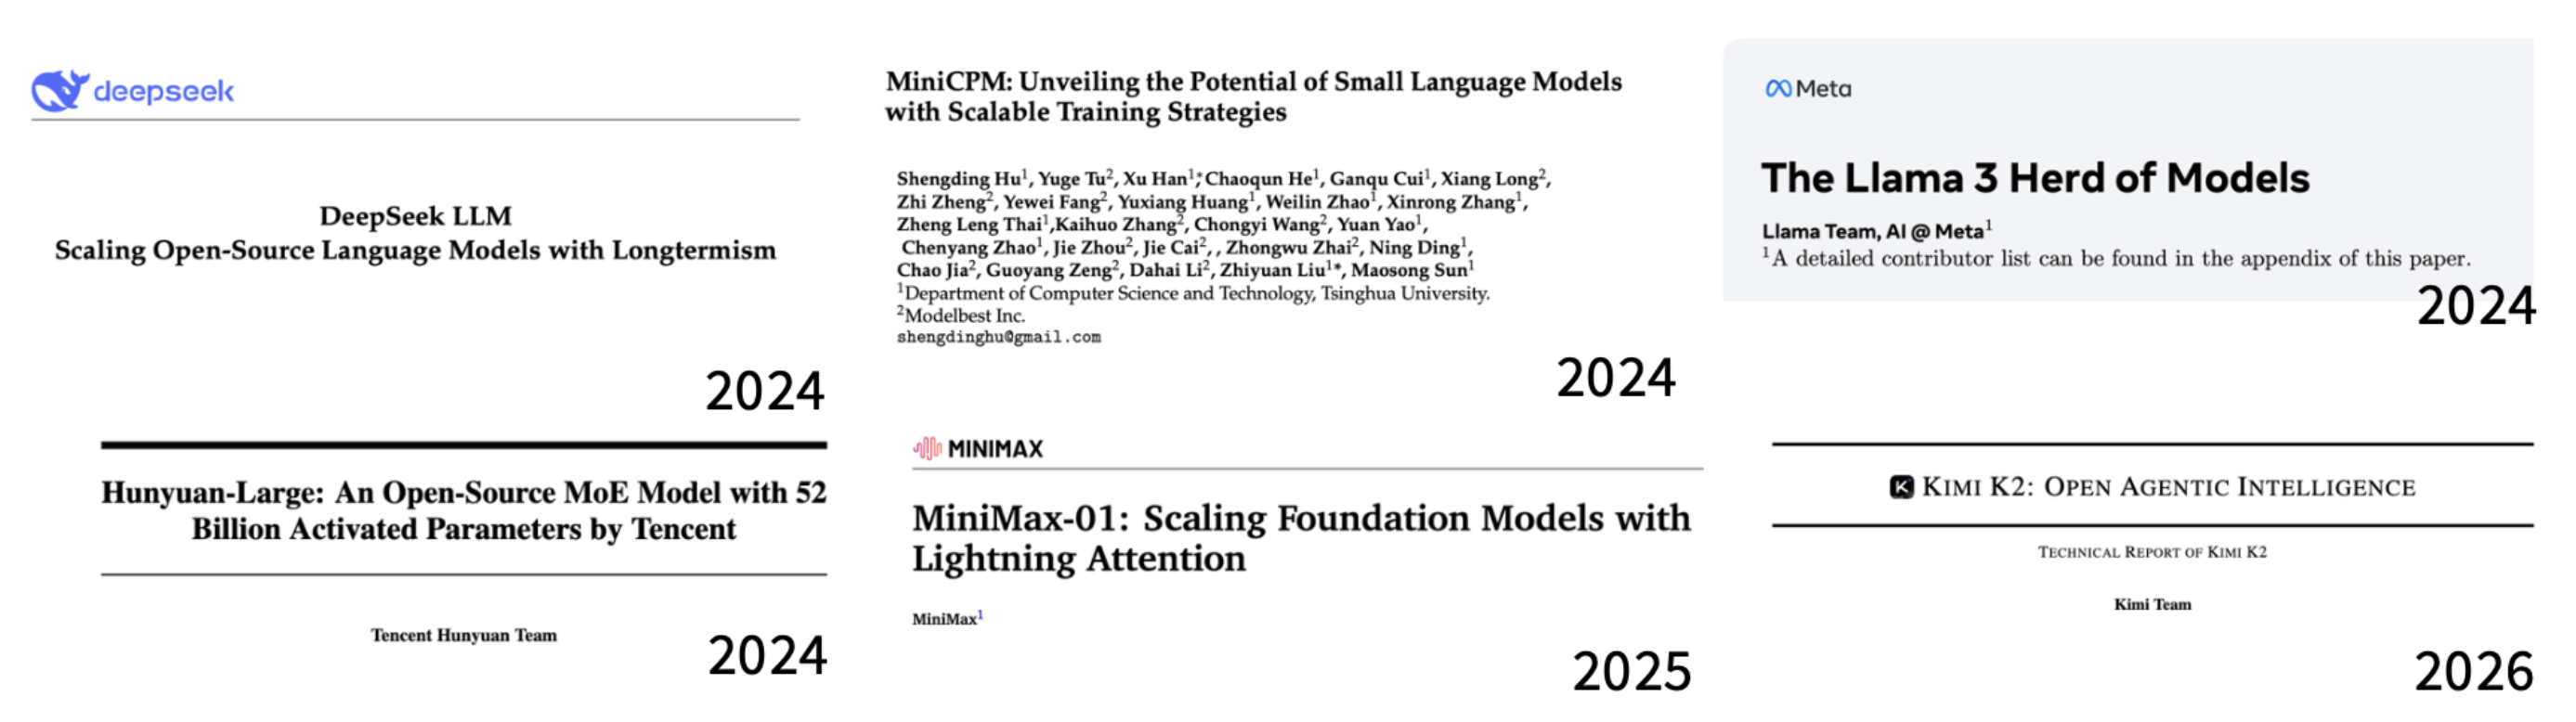
\includegraphics[width=1\linewidth]{deepseek.png}
\end{figure}

\subsubsection*{Initialization and optimization}

\begin{center}
    Initialization, optimizers and various hyperparams (LR/batch) can be scale sensitive!
\end{center}

\begin{figure}[H]
    \centering
    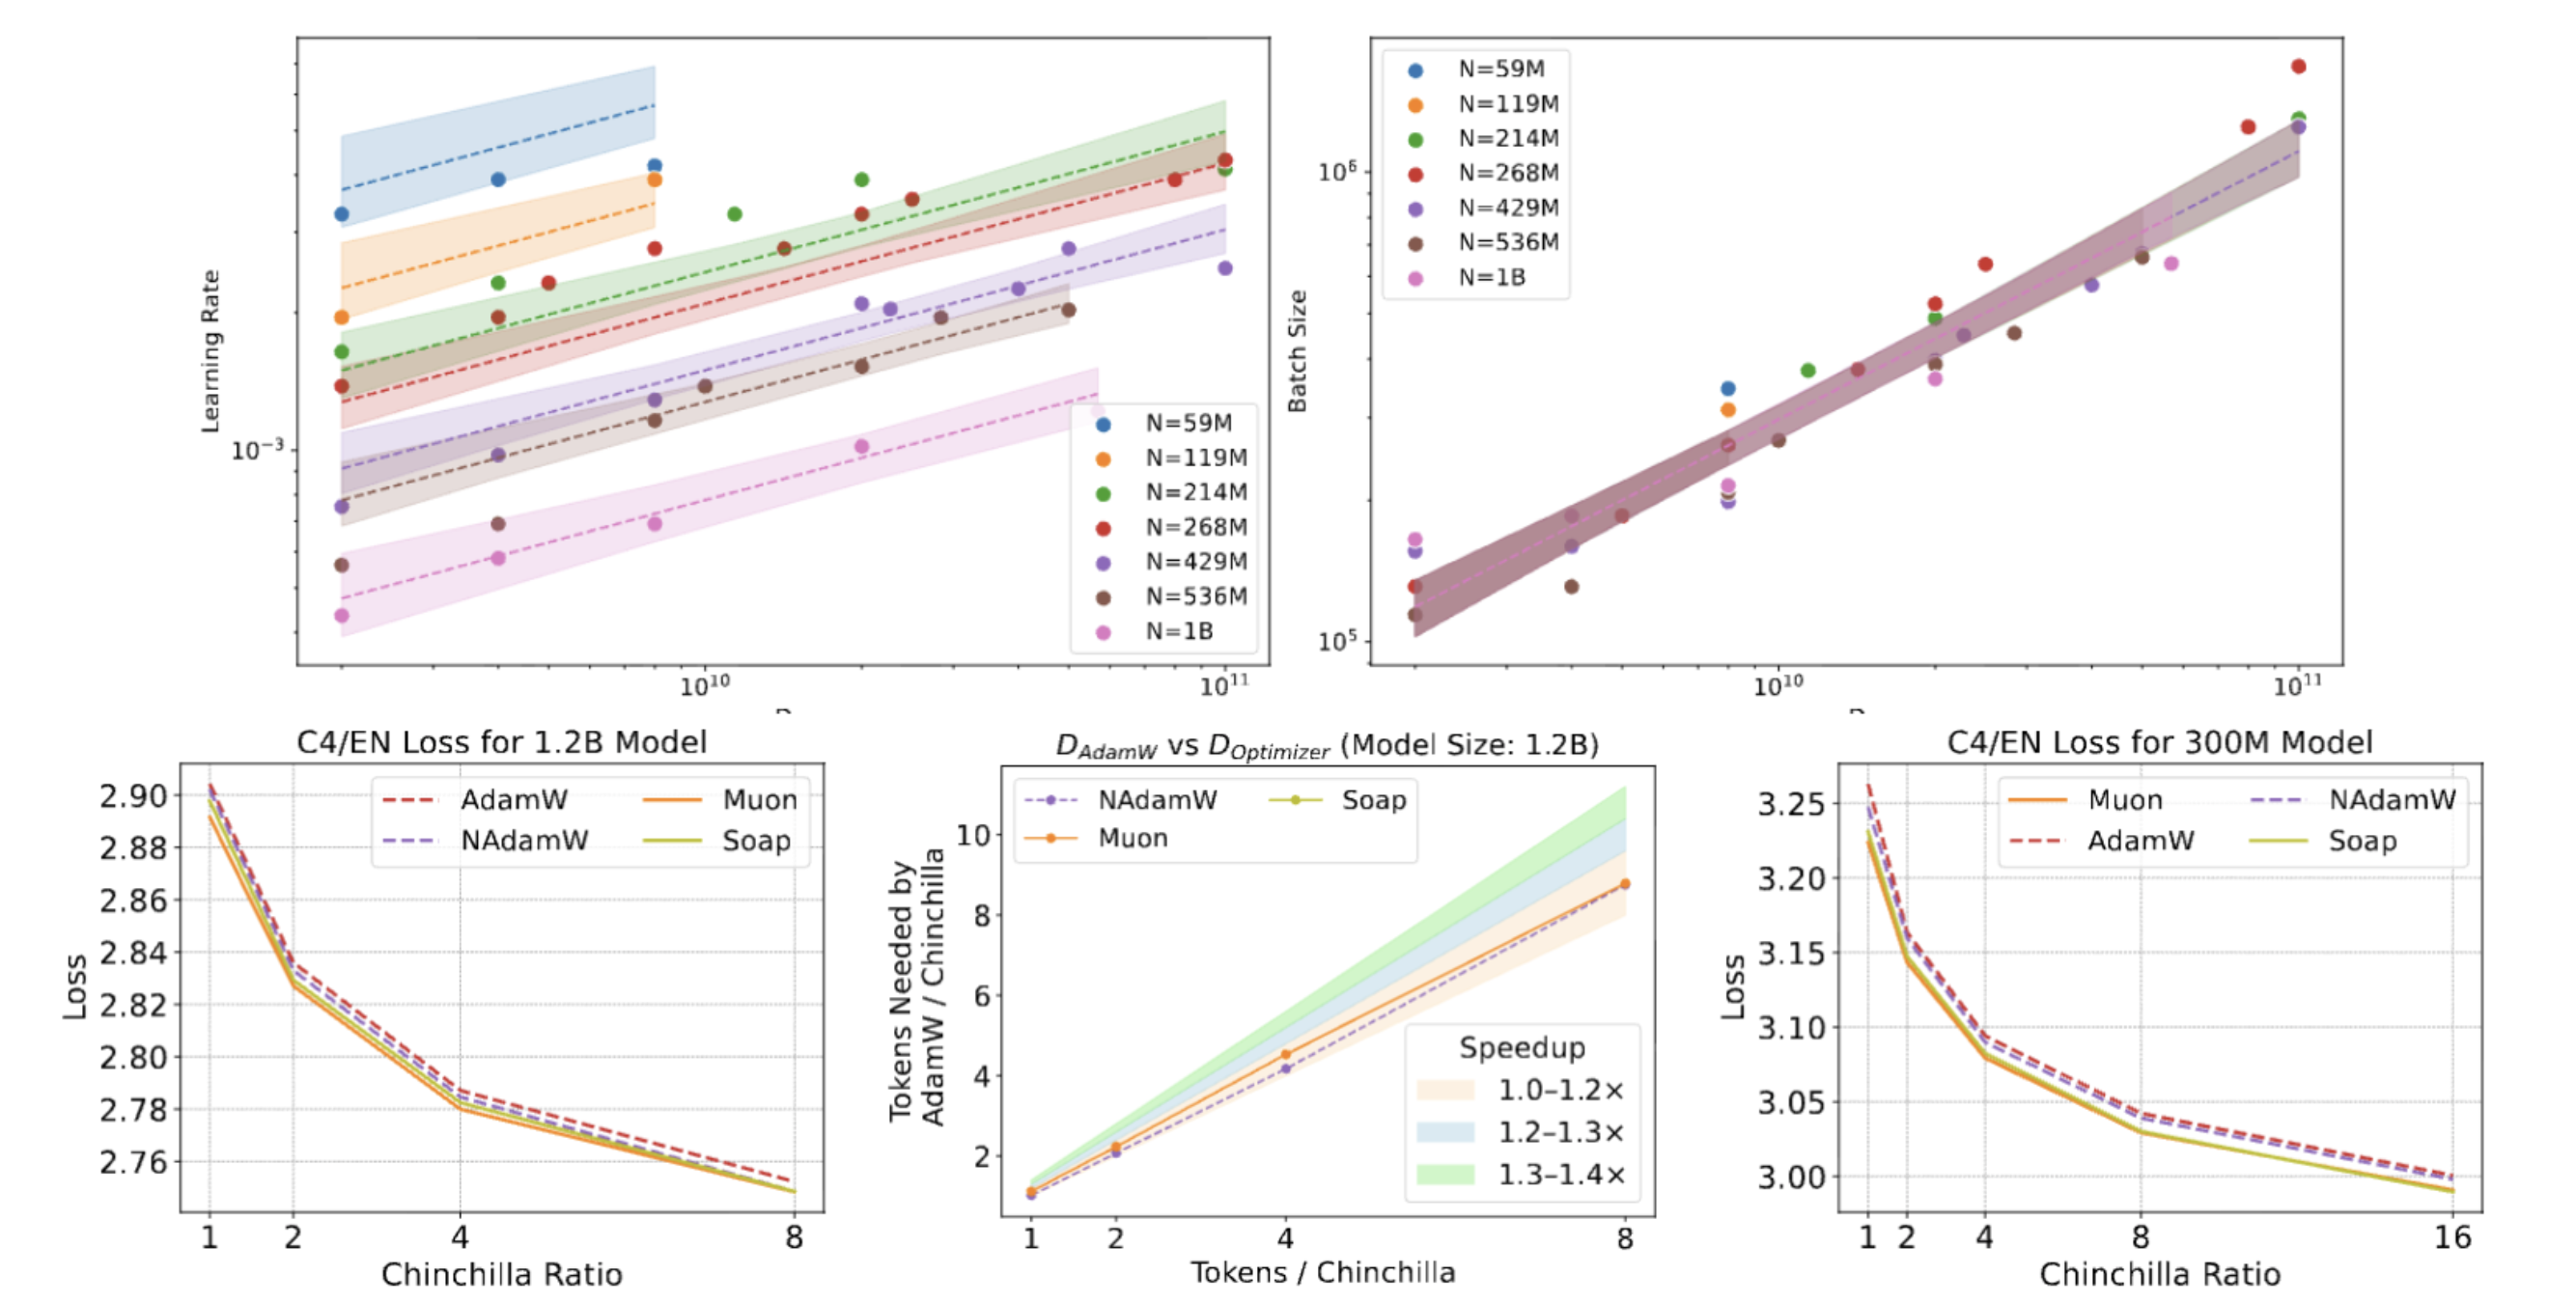
\includegraphics[width=1\linewidth]{init_opt.png}
\end{figure}

\subsubsection*{Working through some detailed, public scaling recipes}

\begin{enumerate}
    \item MiniCPM
    \begin{figure}[hpbt]
        \centering
        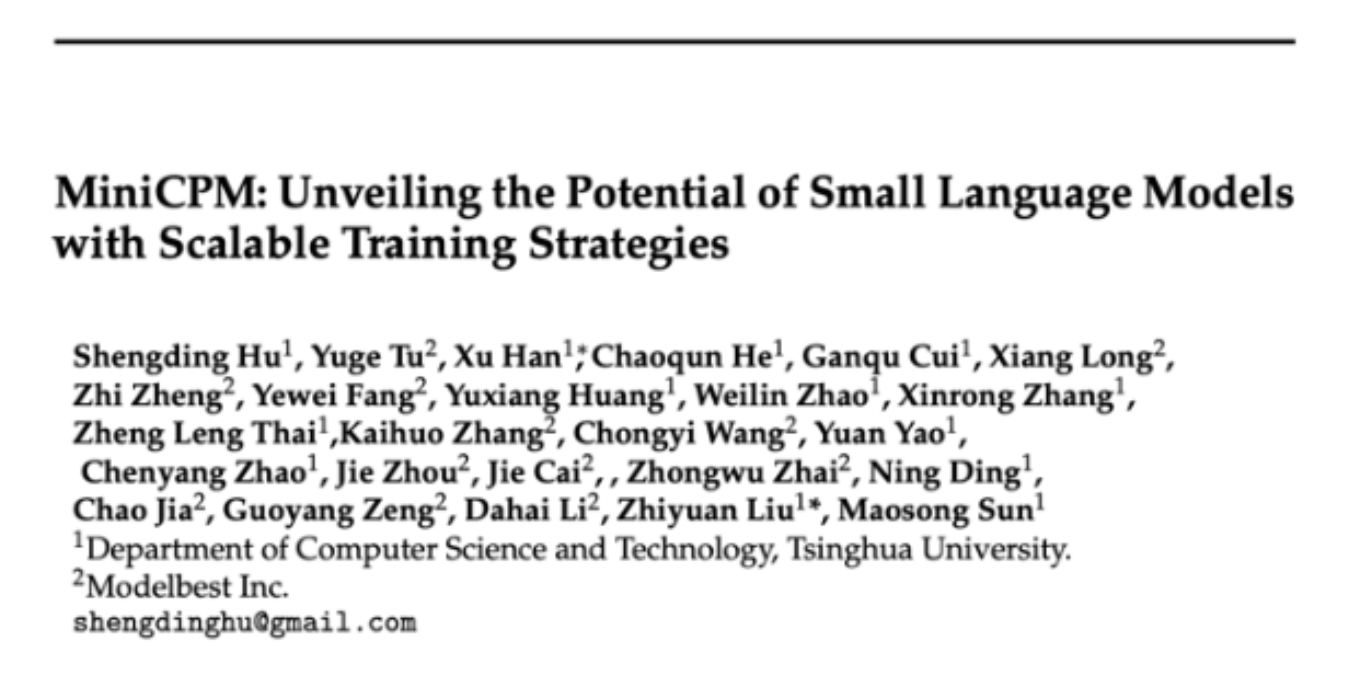
\includegraphics[width=1\linewidth]{cpm_kun.png}
    \end{figure}
    \item DeepSeek
    \begin{figure}[hpbt]
        \centering
        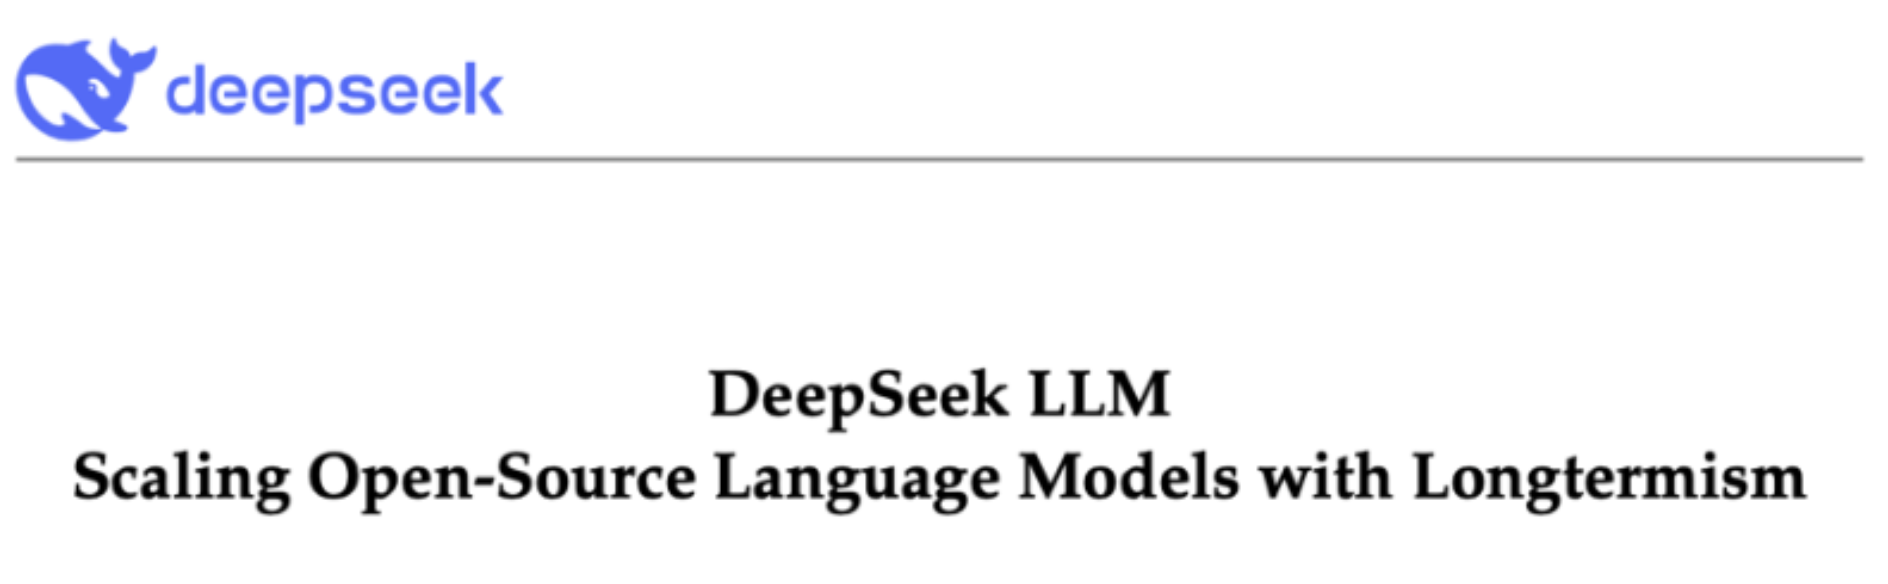
\includegraphics[width=1\linewidth]{ds_kun.png}
    \end{figure}
\end{enumerate}

\subsection*{MiniCPM}

MiniCPM (2024) - small, high-perf LM from Tsinghua group.

\begin{itemize}
    \item Careful, extensive scaling computations \(+\) muP to stabilize and simplify scaling
    \item Not really ``sota'' model (even in 2024) but many interesting lessons on scaling
\end{itemize}

\begin{center}
    High performance 1-2.5B parameter models. These models beat most 2Bs and match many modern 7B models.
\end{center}

\subsubsection*{Technique 1: muP to stabilize scaling}

Scale\_emb \(=\) 12, scale\_depth \(=\) 1.4, init\_std \(=\) 0.1, lr \(=\) 0.01

\begin{enumerate}
    \item Embedding Output Scaling: Multiply the output of the embedding by \textit{scale\_emb}
    \item Residual Connection Scaling: Scale the increment at each residual connection in each layer by \textit{scale\_depth} / \(\sqrt{\operatorname{num\_layers}}\)
    \item Initialization of Tensors: Set the initialization standard deviation of each two-dimensional tensor parameter to \textit{init\_std} / \(\sqrt{d_m / d_{base}}\) and other parameters' initialization to 0.1
    \item Learning Rate Scaling of Tensors: Adjust the learning rate of each two-dimensional tensor parameter to \(1 / (d_m / d_{base})\) times the learning rate of other parts (or the overall learning rate)
    \item LM Head Scaling: Adjust the output logits to \(1 / (d_m / d_{base})\) times the original value
\end{enumerate}

\subsubsection*{Scaling recipe / strategy}

Use muP for initialization, fix the aspect ratio, scale up the overall model size.

\begin{figure}[H]
    \centering
    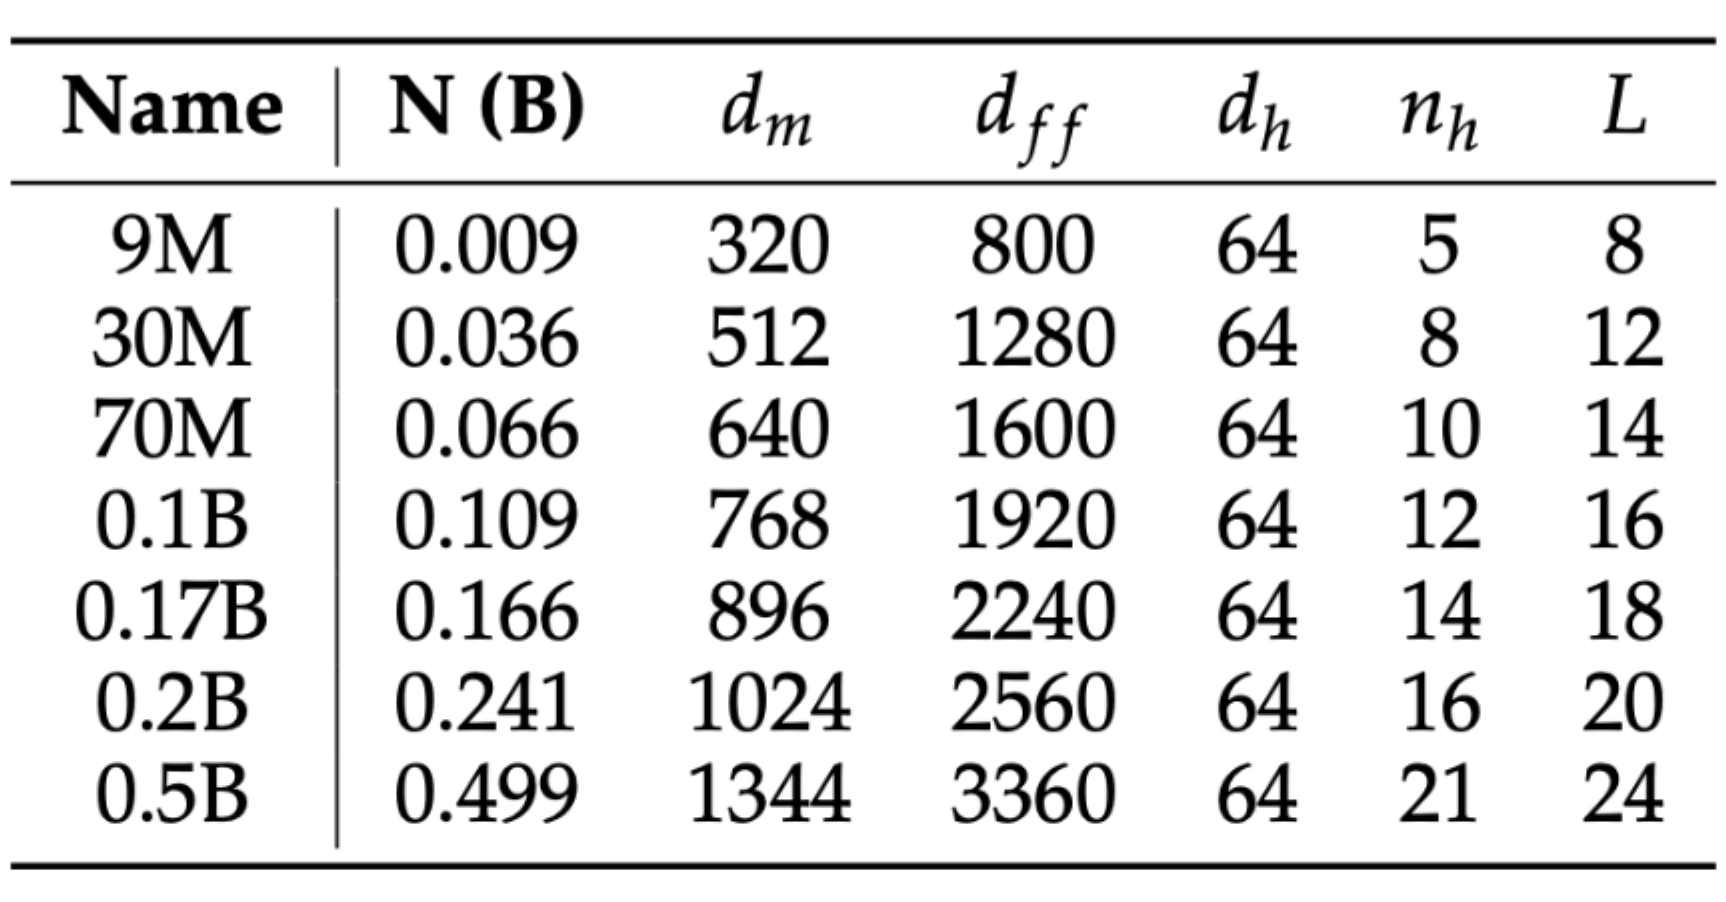
\includegraphics[width=0.75\linewidth]{sizes.png}
\end{figure}

Note that the gap between the largest model here and the actual model they train is 5\(\times\).

\begin{center}
    Optimal batch, LR, token-to-size ratios are directly fitted via scaling analysis.
\end{center}

\subsubsection*{Optimal LR}

According to muP - optimal learning rate should be (roughly) stable. Is it?

\begin{figure}[hpbt]
    \centering
    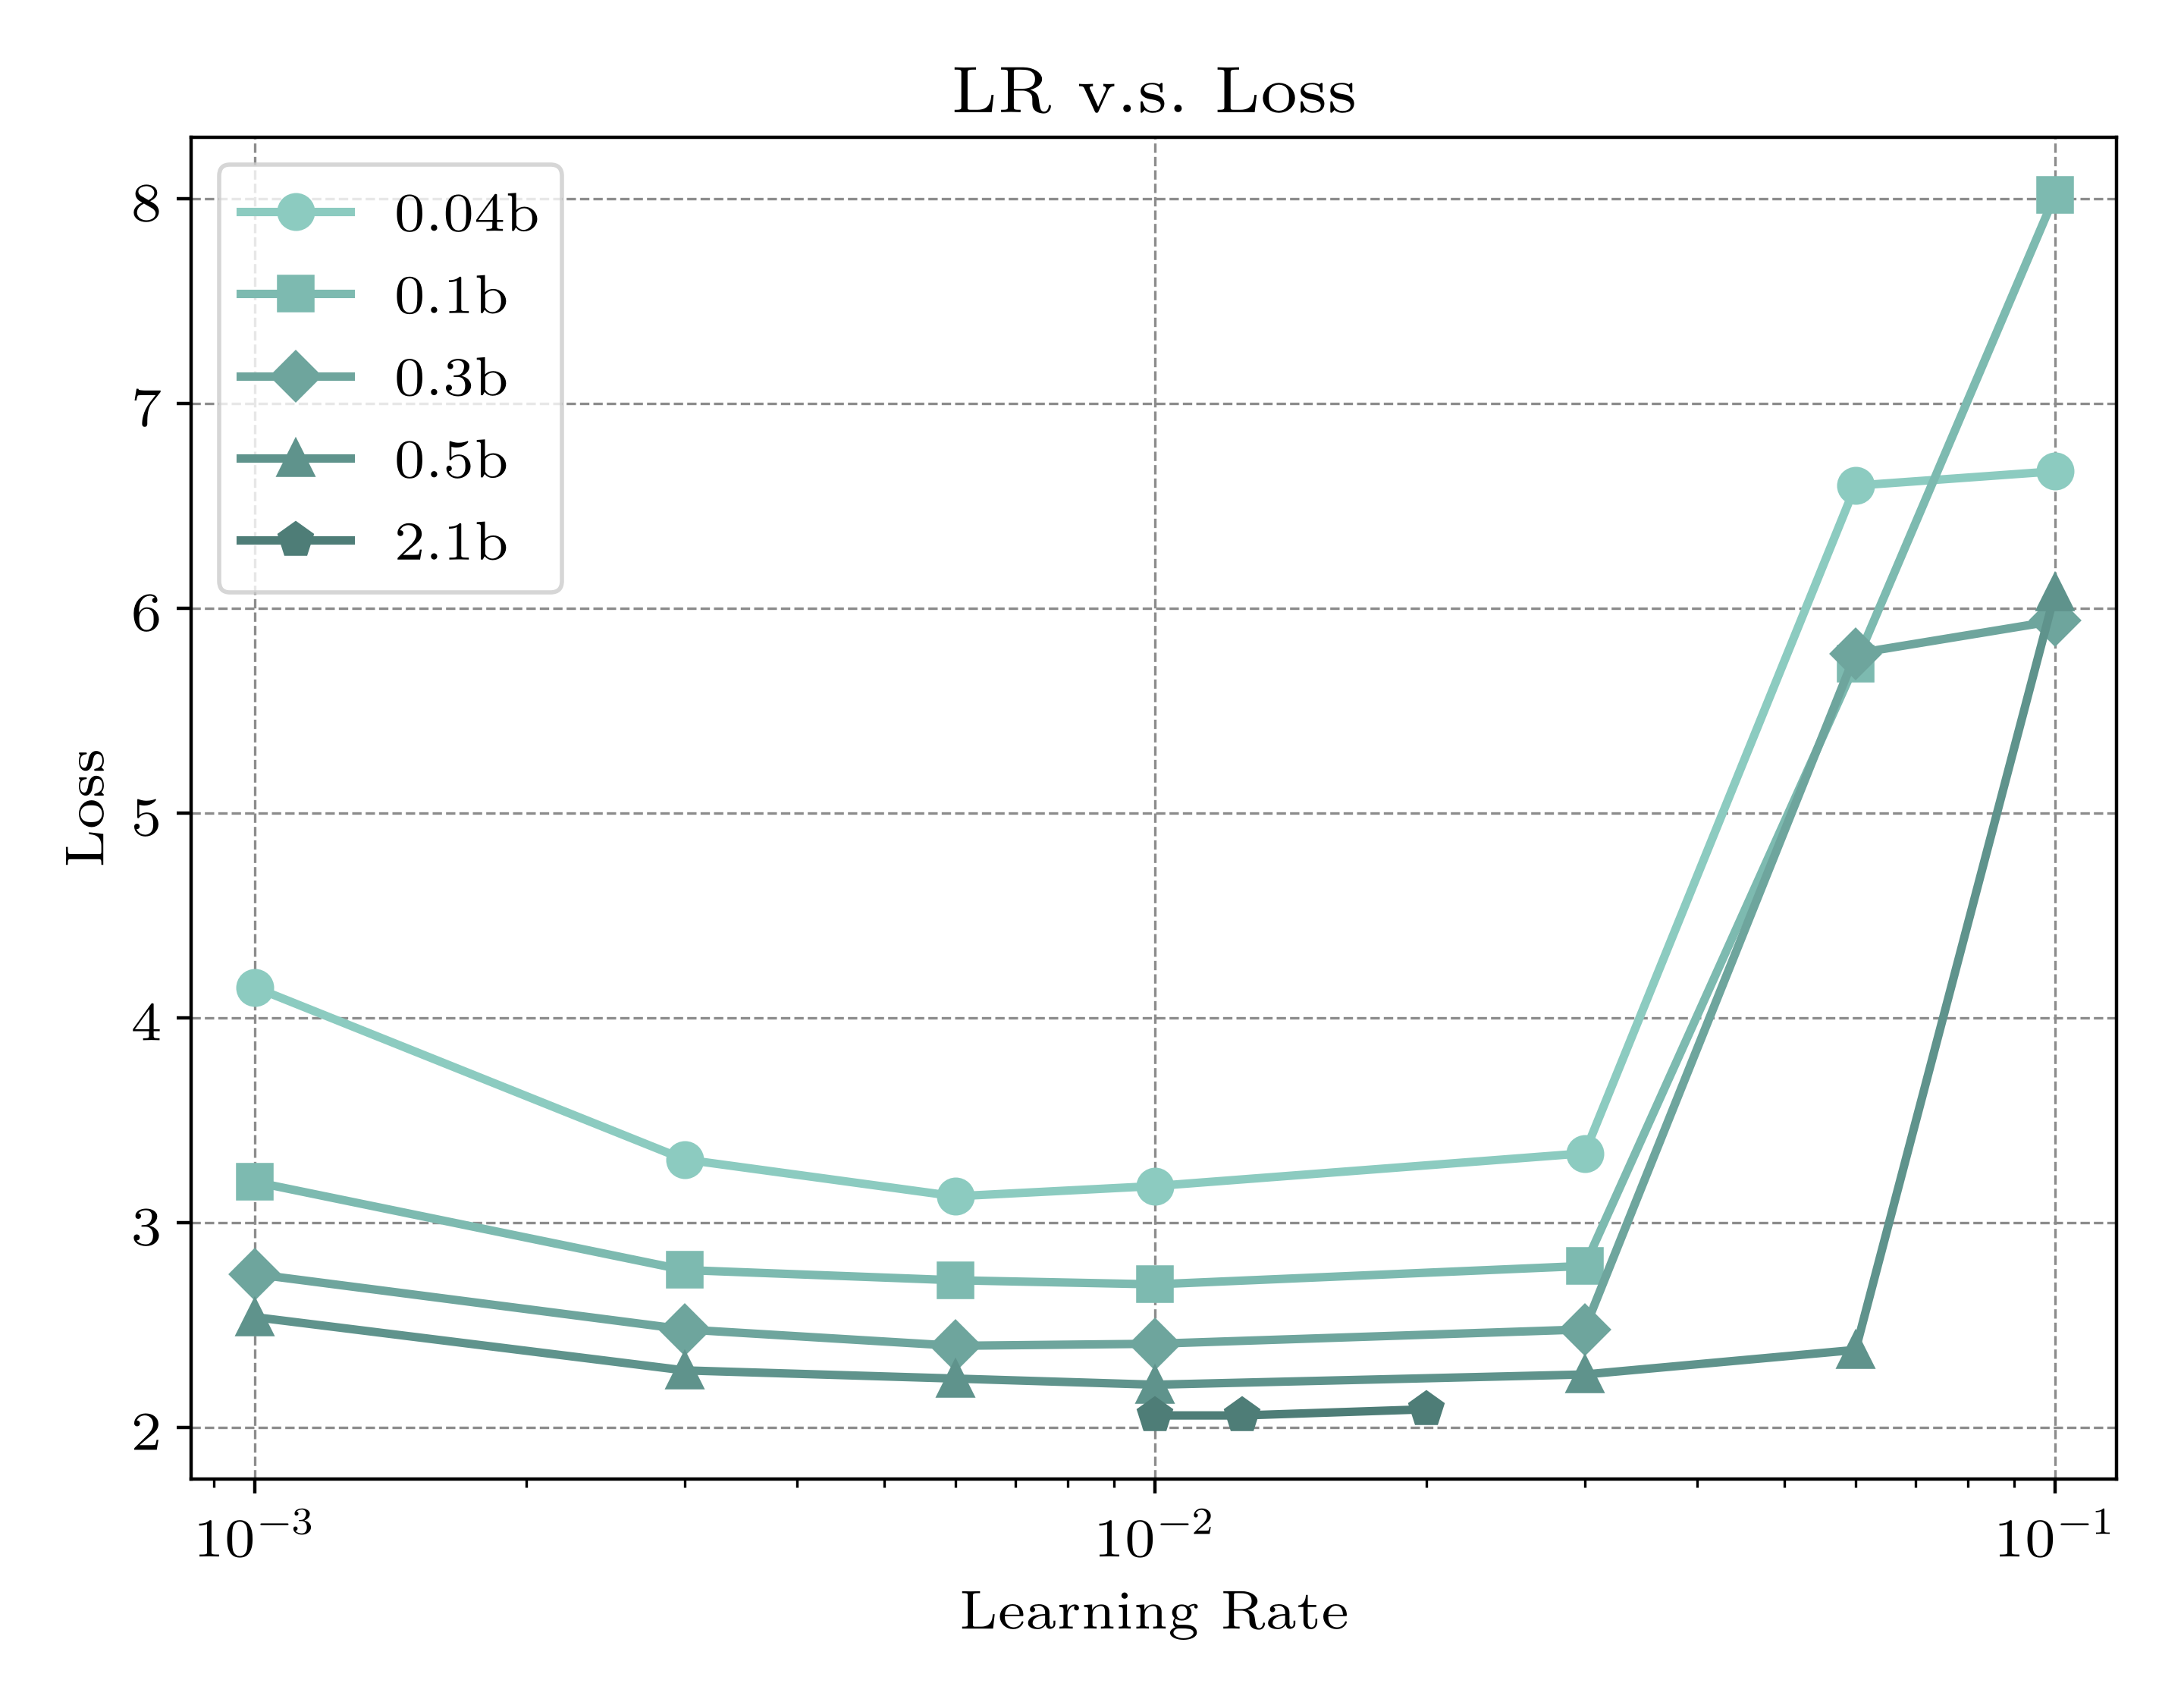
\includegraphics[width=0.68\linewidth]{lr_vs_loss.png}
\end{figure}

\subsubsection*{Optimal batch size}

Three model sizes (9m, 30m, 170m) as a function of batch (x), data size (y) and loss (col).

\begin{itemize}
    \item Vertical columns of points represent a single training curve (fixed batch, more points).
    \item Red line attempts to identify minimum loss points for each y-value.
    \item This is the ``optimal batch size'' for a model size / dataset size combination.
\end{itemize}

We can then follow the Kaplan 2020 analysis and plot batch size vs final loss.

\hfill

Fairly clean trend - polynomially increase the batch size as loss decreases.

\subsubsection*{What remains - model size vs data tradeoffs}

From Chinchilla - to fit a scaling law, we need to train from scratch, not just early stop.

\begin{figure}[hpbt]
    \centering
    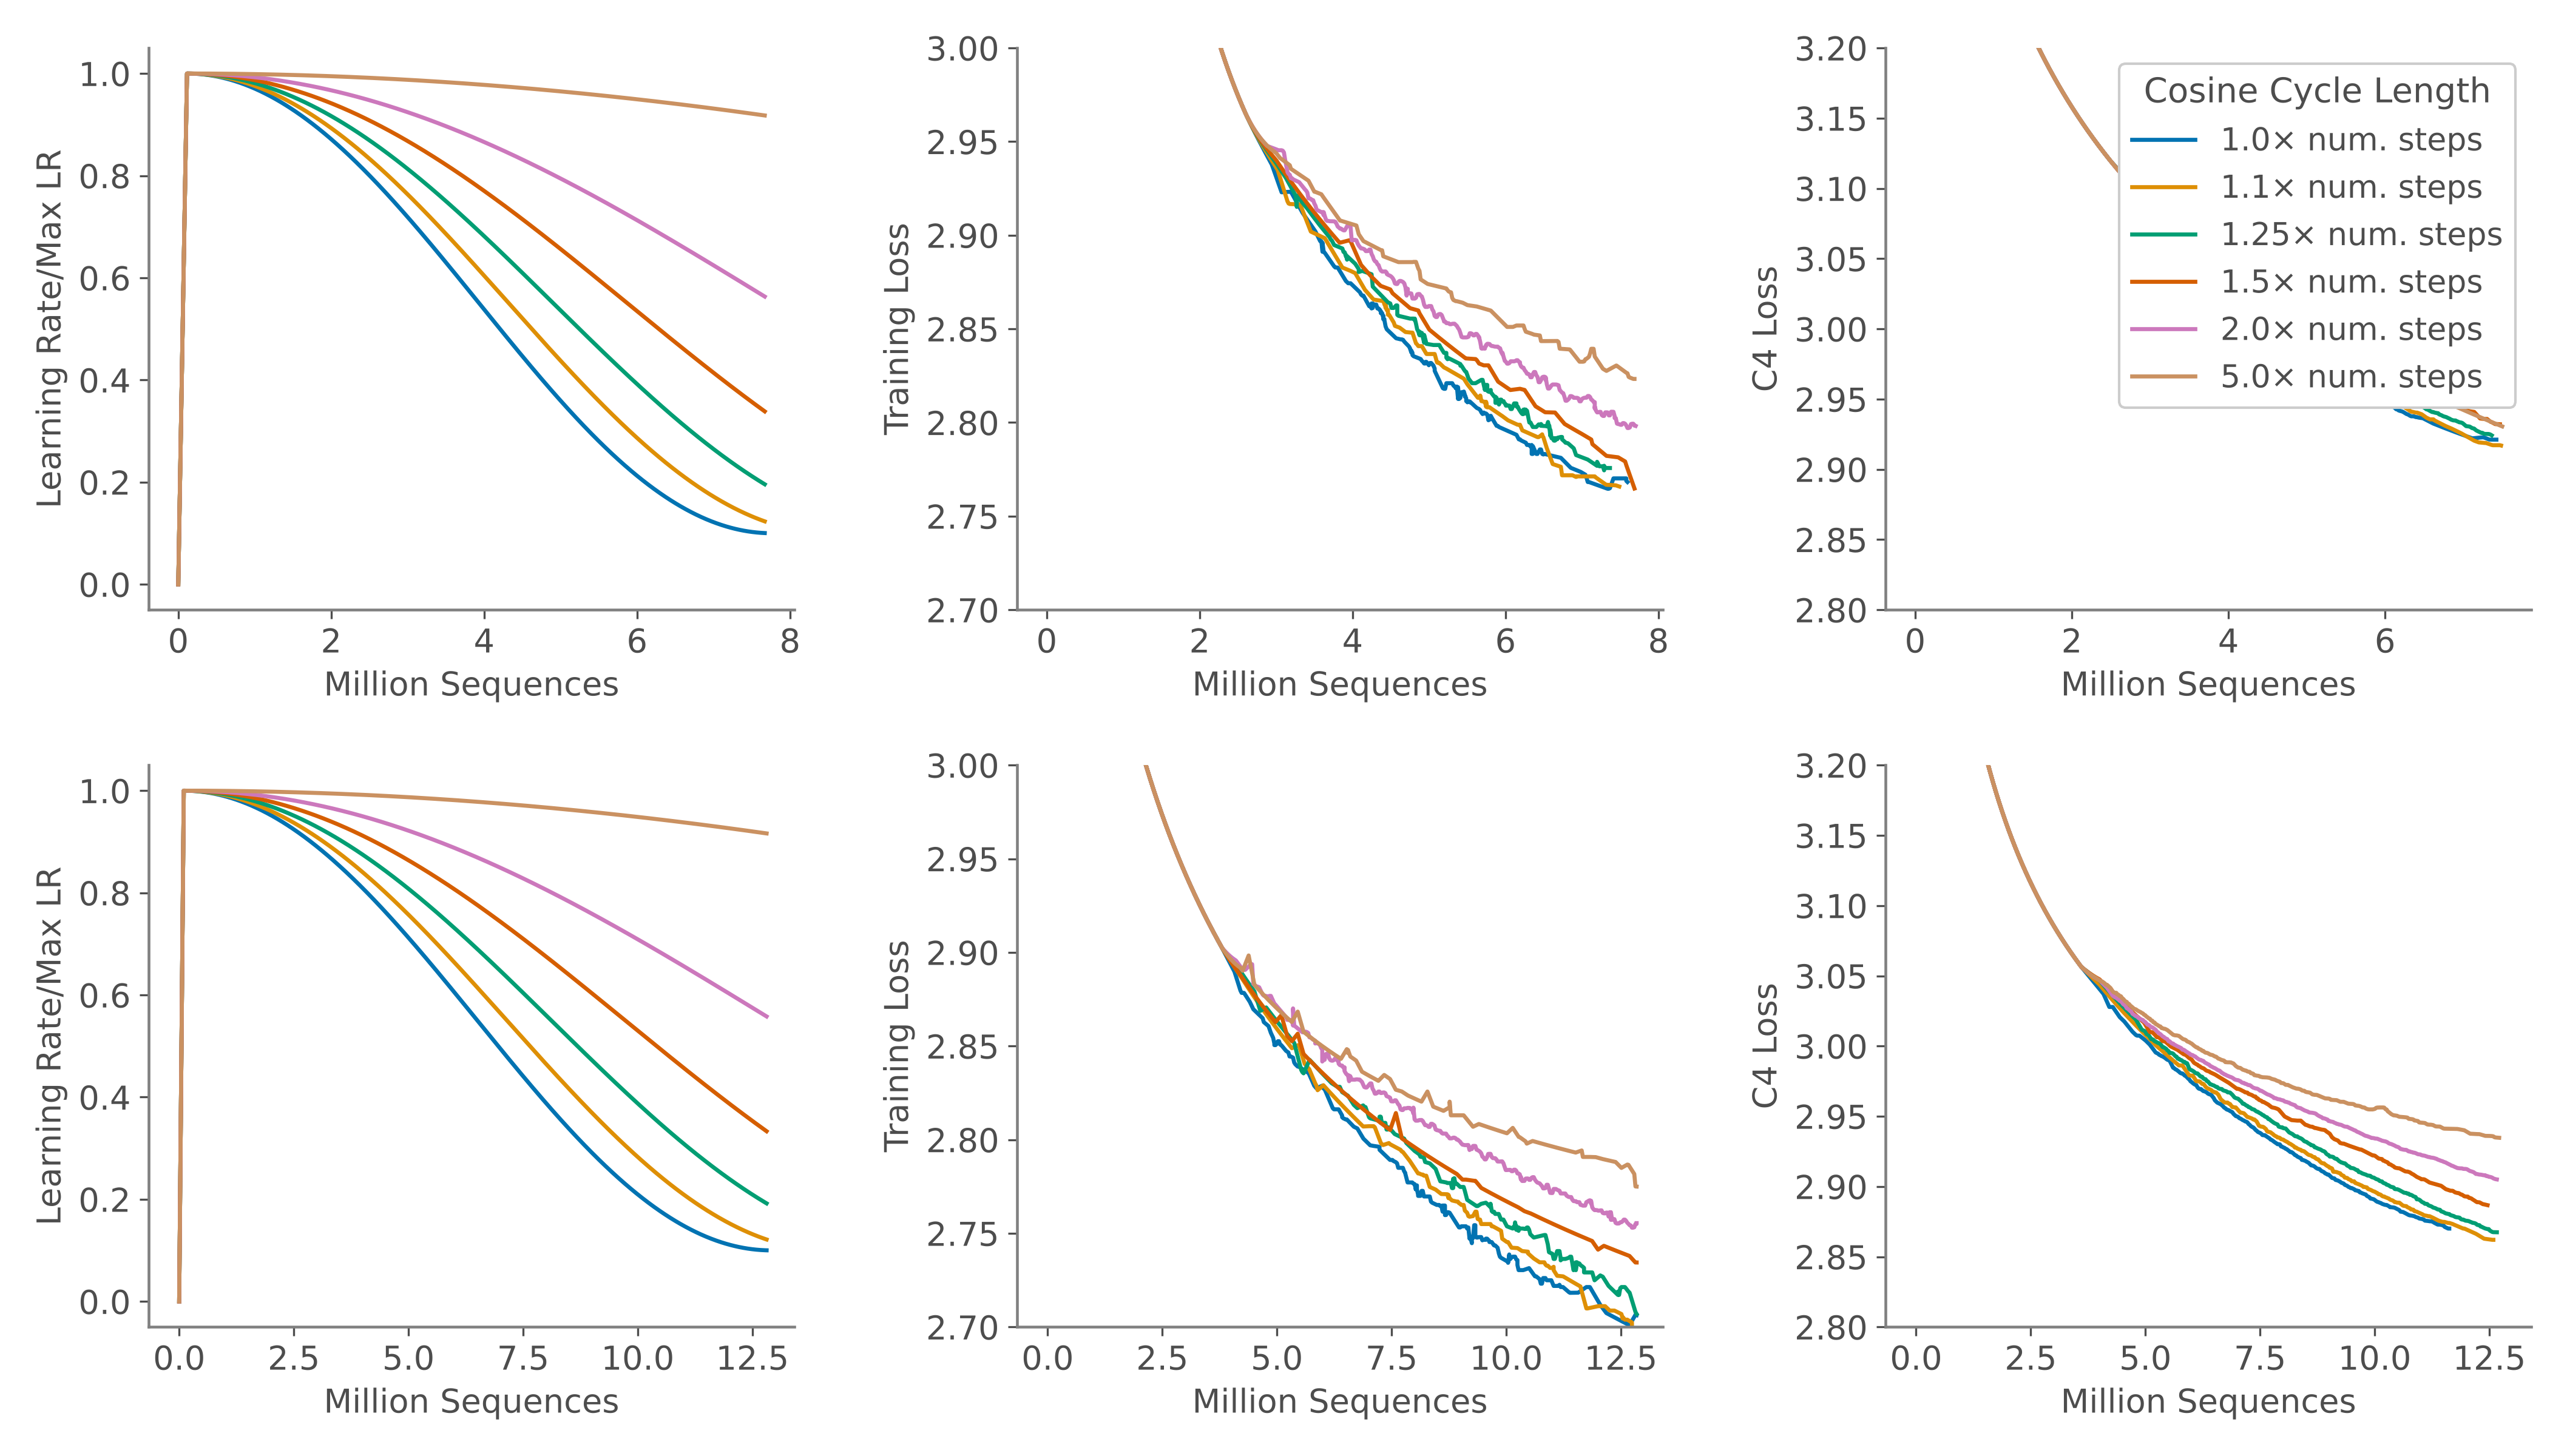
\includegraphics[width=1\linewidth]{cosine_cycle_length.png}
\end{figure}

This turns the cost of fitting a scaling law from \(n\) to \(n^2\). Can we avoid this?

\subsubsection*{(partial) solution in miniCPM - WSD learning rate}

Instead of cosine, split learning rate into warmup, stable and decay phases.

\begin{figure}[H]
    \centering
    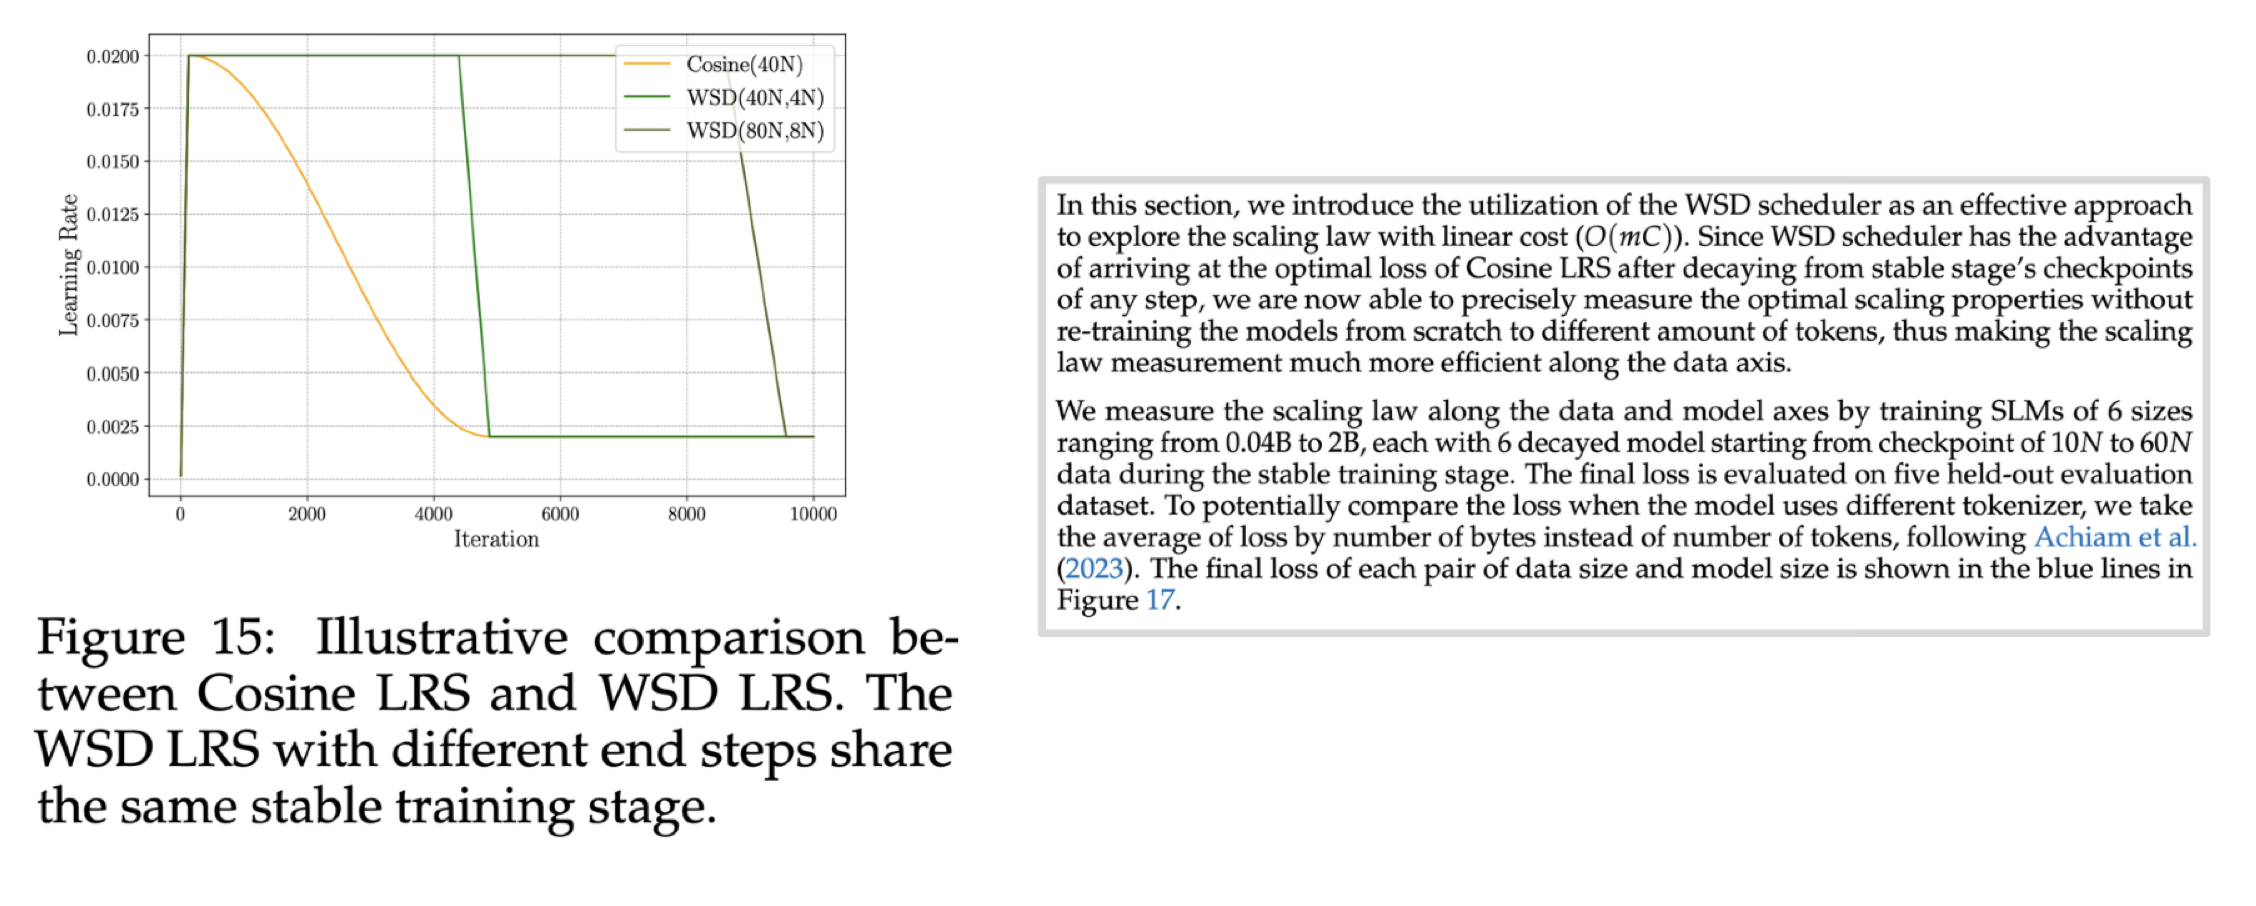
\includegraphics[width=1\linewidth]{WSD.png}
\end{figure}

For Chinchilla-style analysis, can restart the run at the end of the stable phase.

\subsubsection*{WSD learning rates work well in miniCPM}

Slower during the stable phase, rapid loss decay during decay phase. Decay 10\%.

\begin{figure}[hpbt]
    \centering
    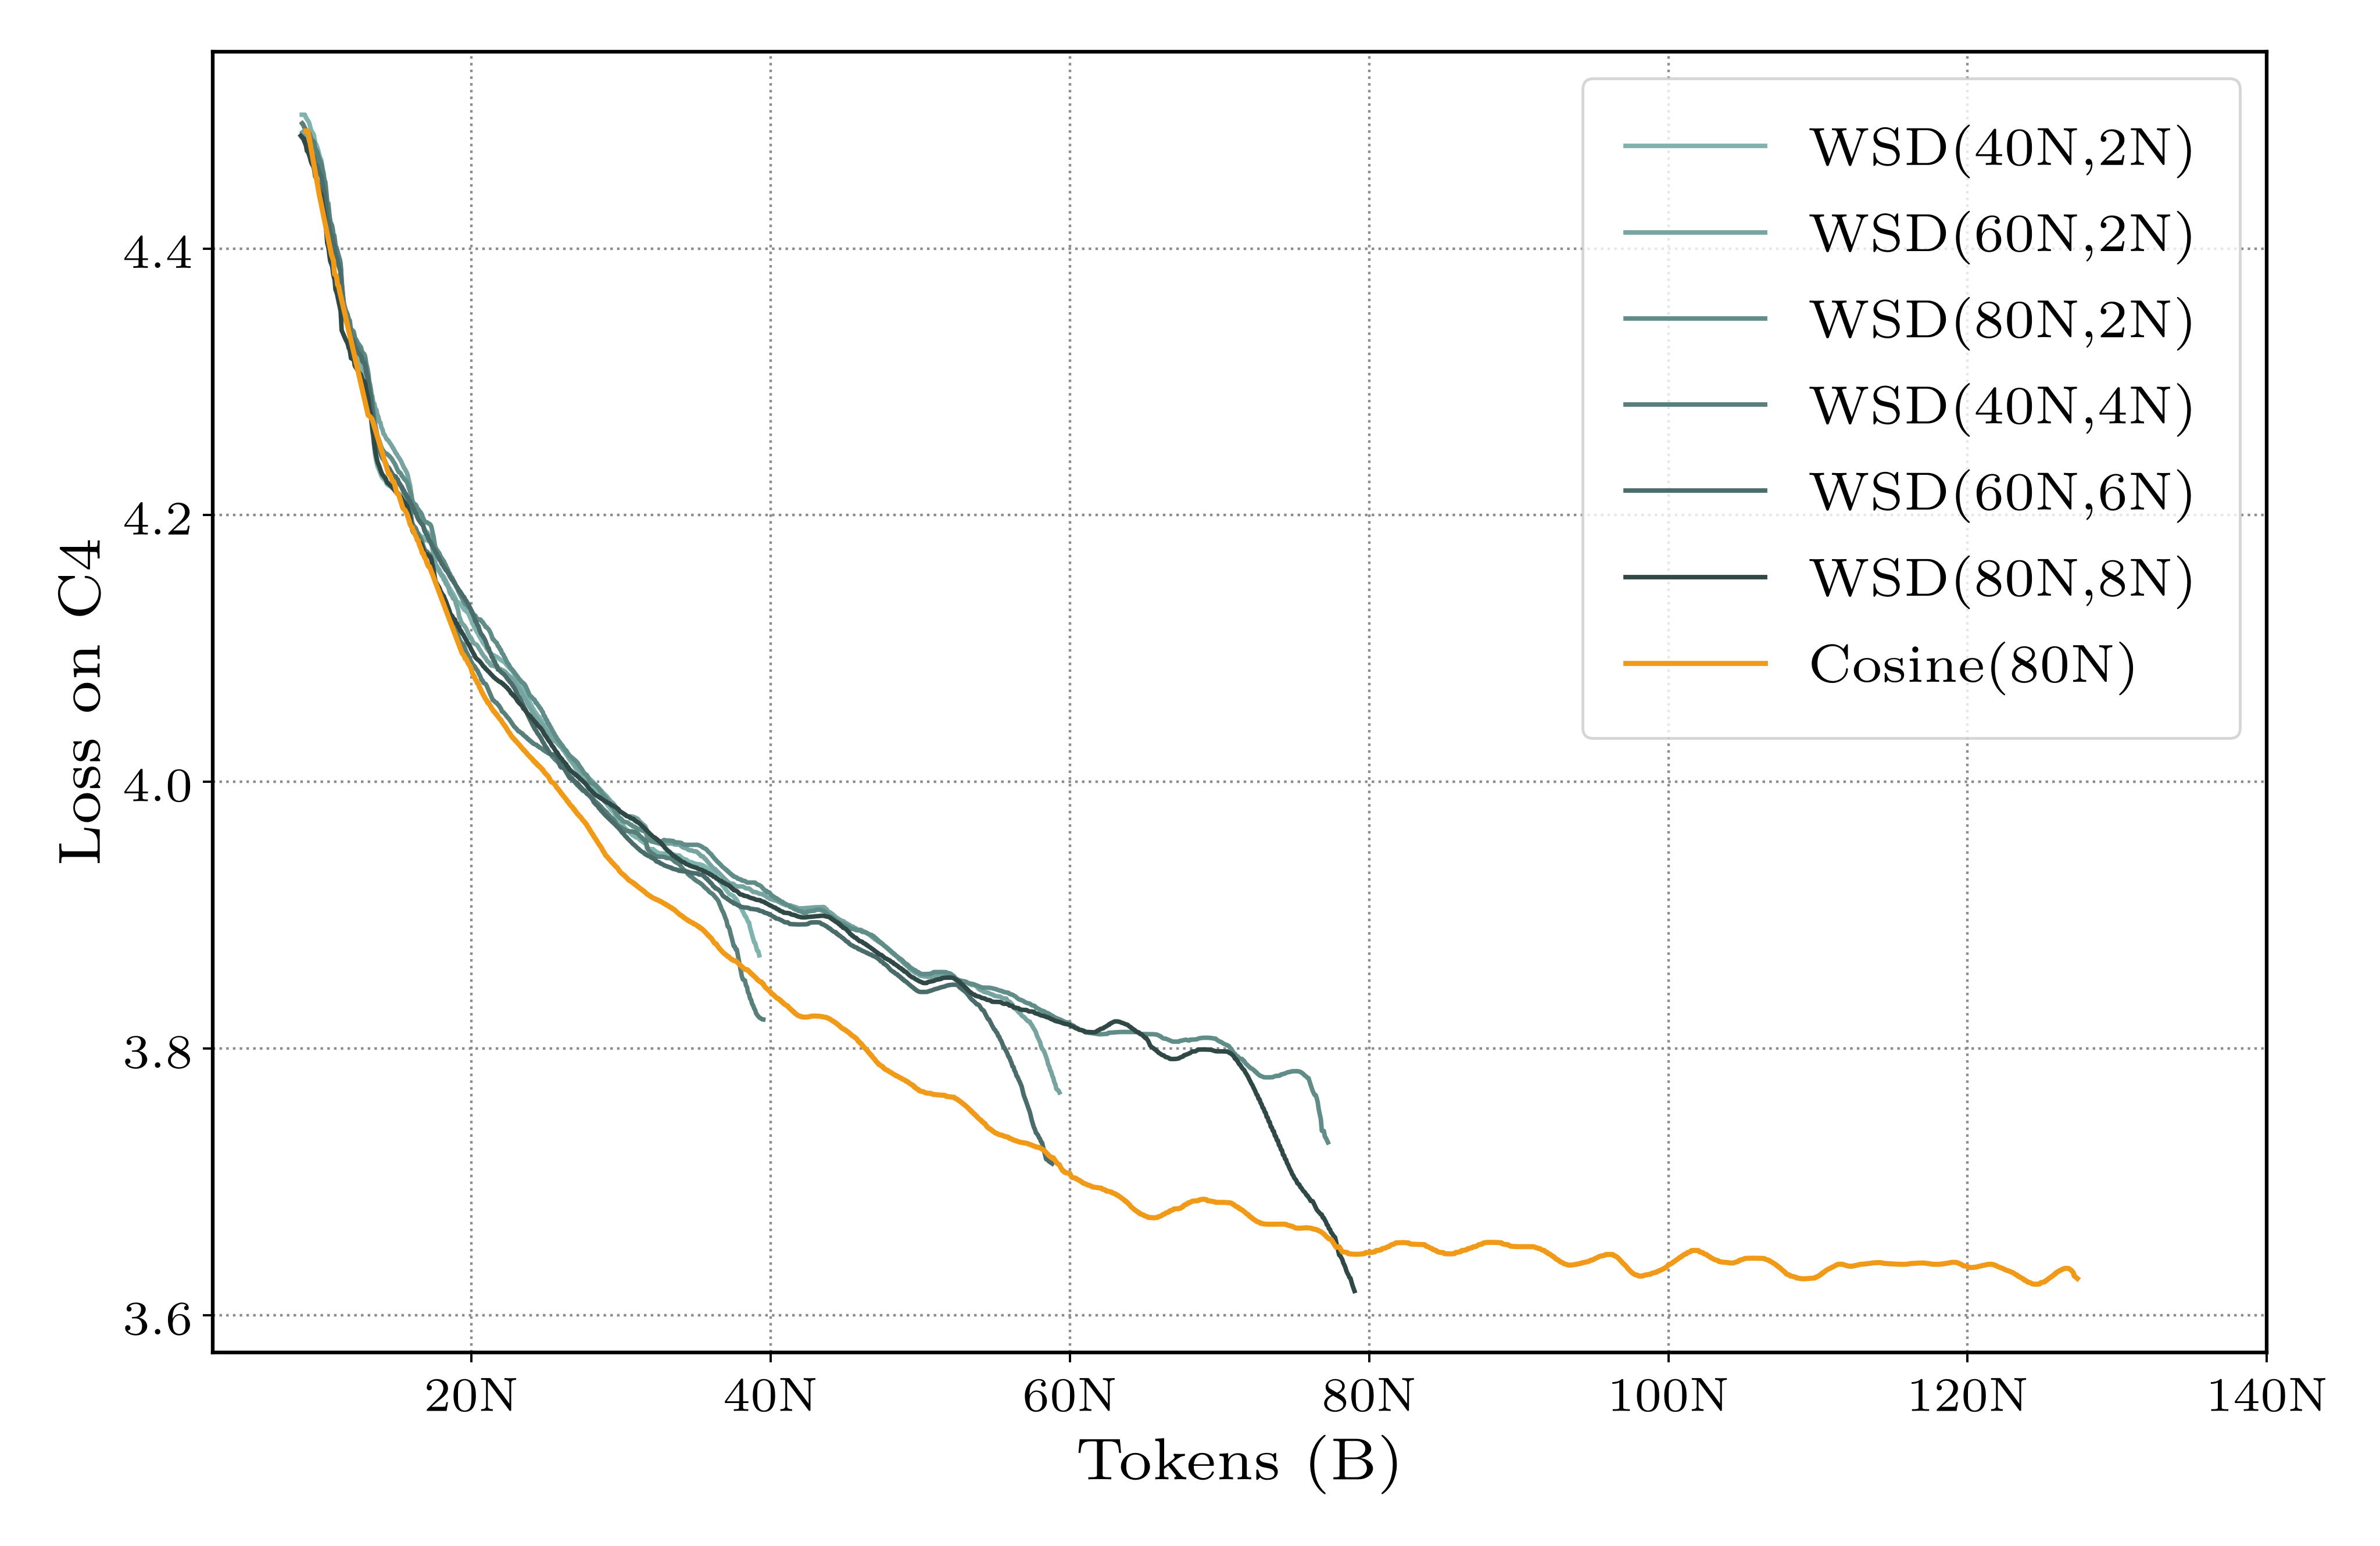
\includegraphics[width=0.5\linewidth]{wsd_vs_cosine.png}
\end{figure}

\subsubsection*{Chinchilla-type analysis}

Equipped with the WSD learning rate, we can now try to find the optimal data-to-model size ratio:
\[
    L(N,D) = C_N N^{-\alpha} + C_D D^{-\beta} + L_0.
\]

MiniCPM authors choose the first method (lower envelope) and third method (joint fit):
\[
    \frac{N_{\operatorname{opt}}}{D_{\operatorname{opt}}} = K^2 \left(\frac{C}{6}\right)^{\eta}.
\]

\subsection*{DeepSeek}

DeepSeek (2024) - another LM with careful scaling analysis

\begin{itemize}
    \item 7 and 67B param models - generally high performance compared to other open LMs
    \item \textbf{Scaling strategy}: don't use any muP, directly estimate optimal batch / LR
\end{itemize}

\begin{figure}[hpbt]
    \centering
    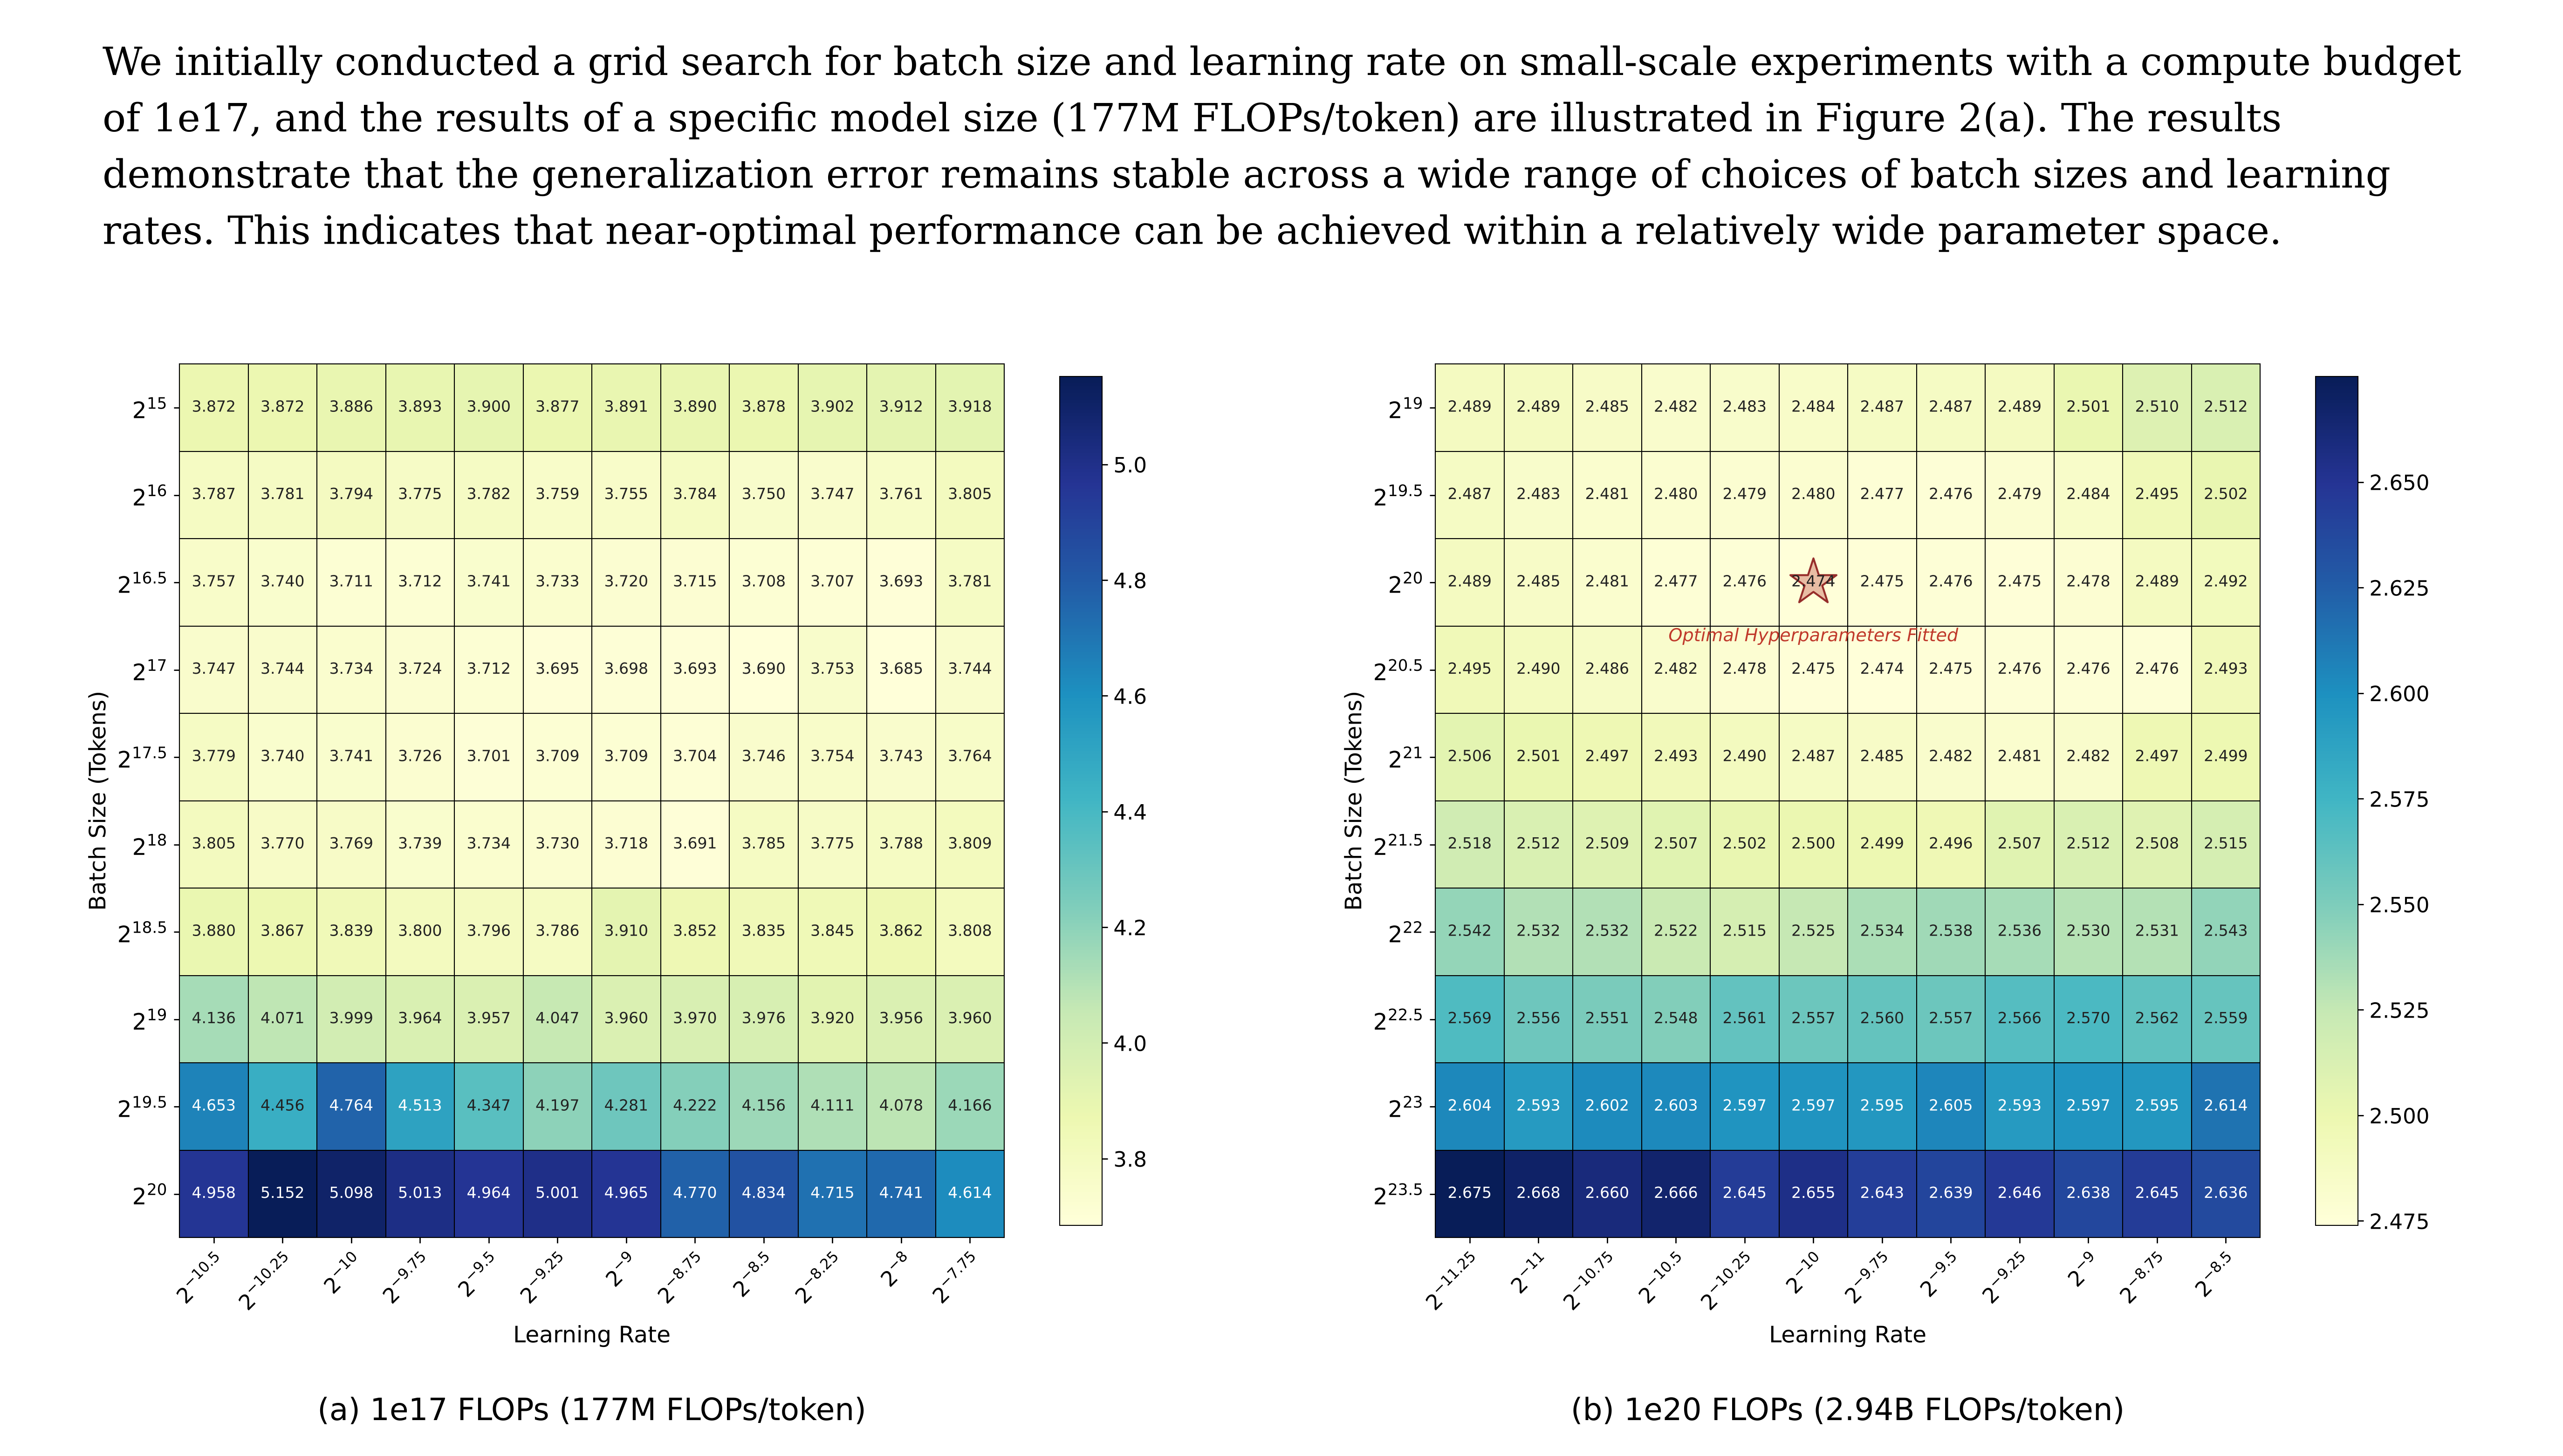
\includegraphics[width=1\linewidth]{figure2_hires.png}
\end{figure}

Small scale runs \(+\) collect ``near optimal'' (within 0.25\% of min) models.
\begin{align*}
    \eta_{\operatorname{opt}} &= 0.3118 \cdot C^{-0.1250} \\
    B_{\operatorname{opt}} &= 0.2920 \cdot C^{0.3271}
\end{align*}

\begin{figure}[hpbt]
    \centering
    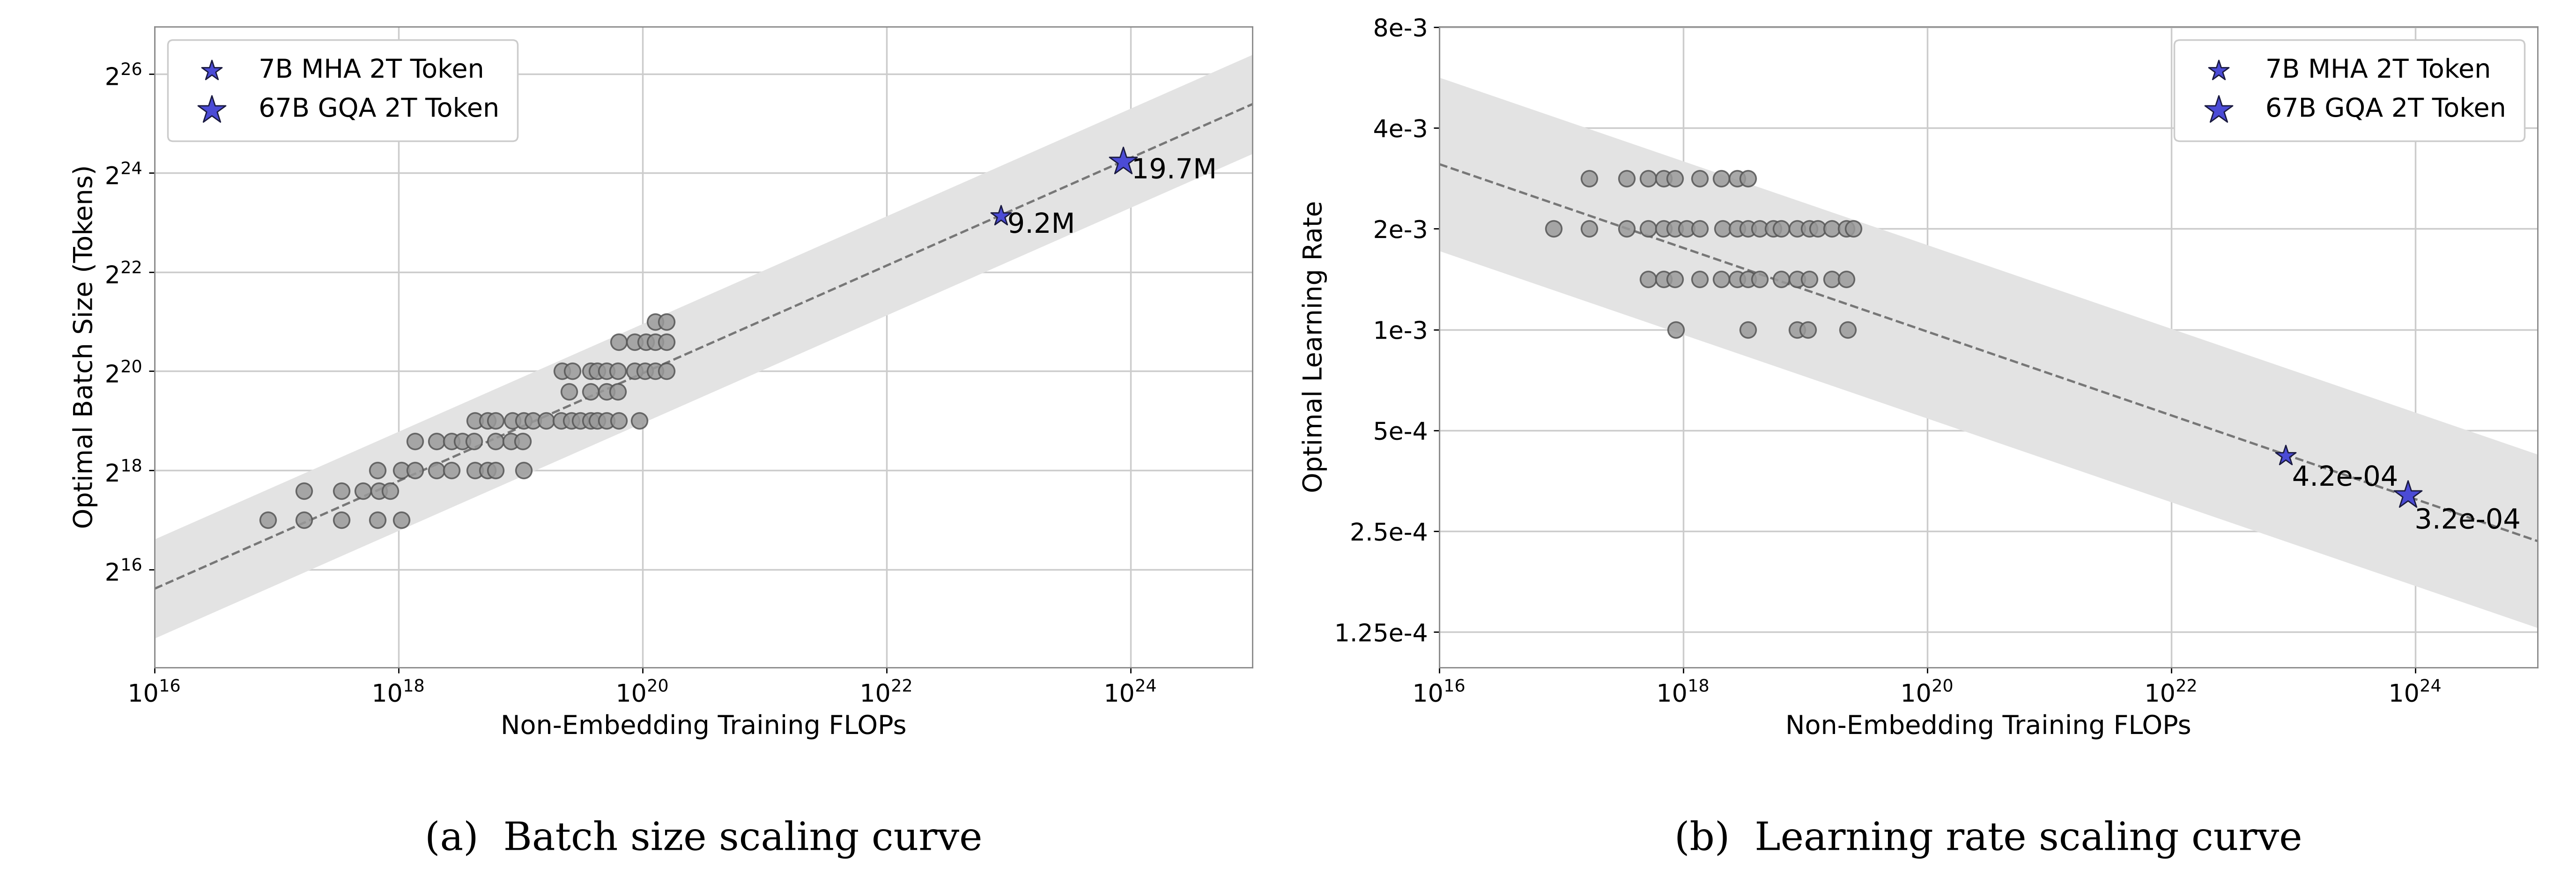
\includegraphics[width=0.8\linewidth]{figure3_hires.png}
\end{figure}

Learning rate fit looks a bit questionable\ldots

\subsubsection*{WSD-style learning rate}

DeepSeek uses WSD-style learning rate \(\to\) fast warmup \(+\) two decay steps of 10\% each.

\hfill

Generally seems to match performance of cosine learning rates.

\subsubsection*{Data-size tradeoff: Chinchilla second method}

Straightforward IsoFLOP-style analysis for selecting the model size tradeoffs.

\begin{figure}[hpbt]
    \centering
    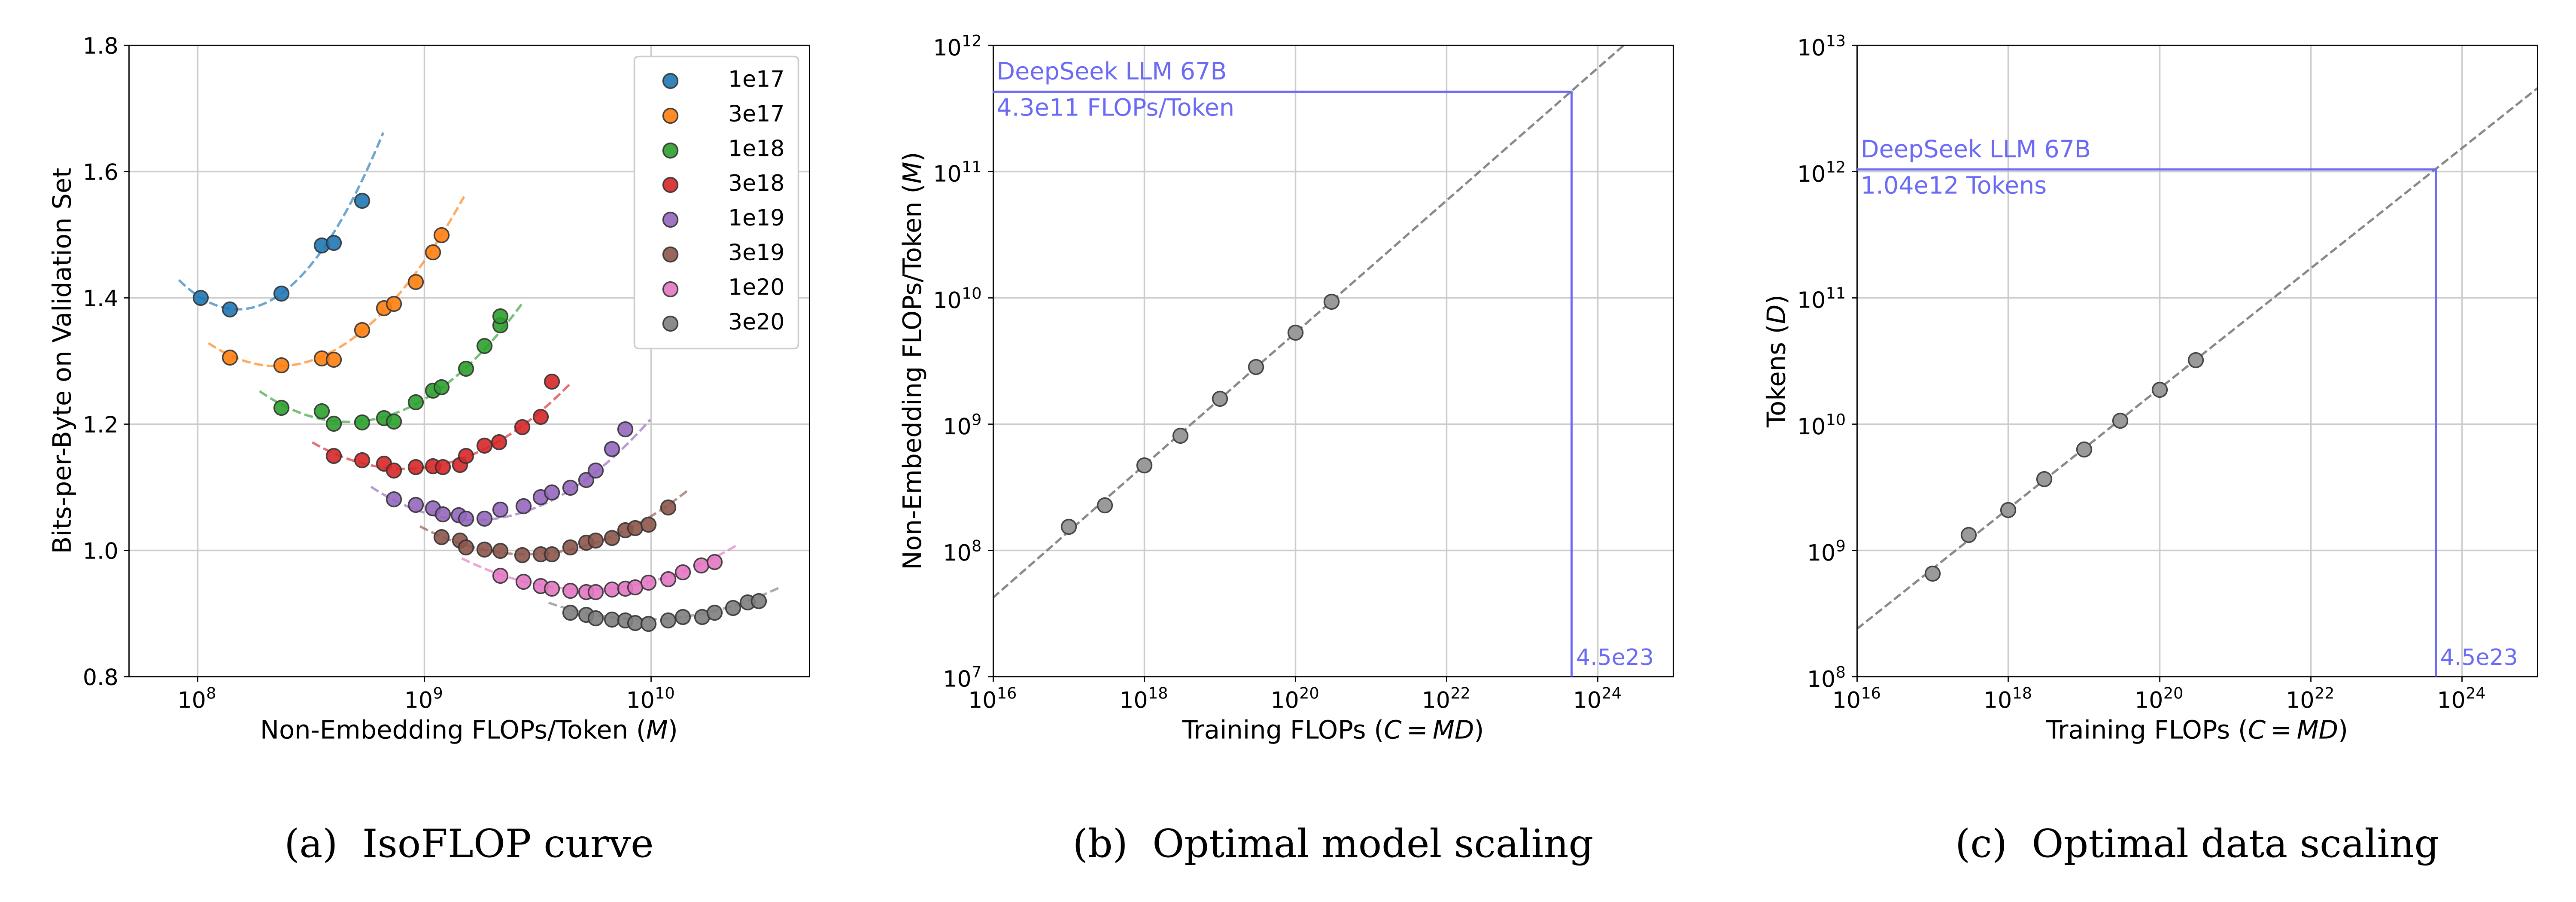
\includegraphics[width=1\linewidth]{figure4_hires.png}
\end{figure}

\subsubsection*{Scaling predicts final model loss}

The fitted scaling models (generally) accurately predict the final model losses.

\begin{figure}[hpbt]
    \centering
    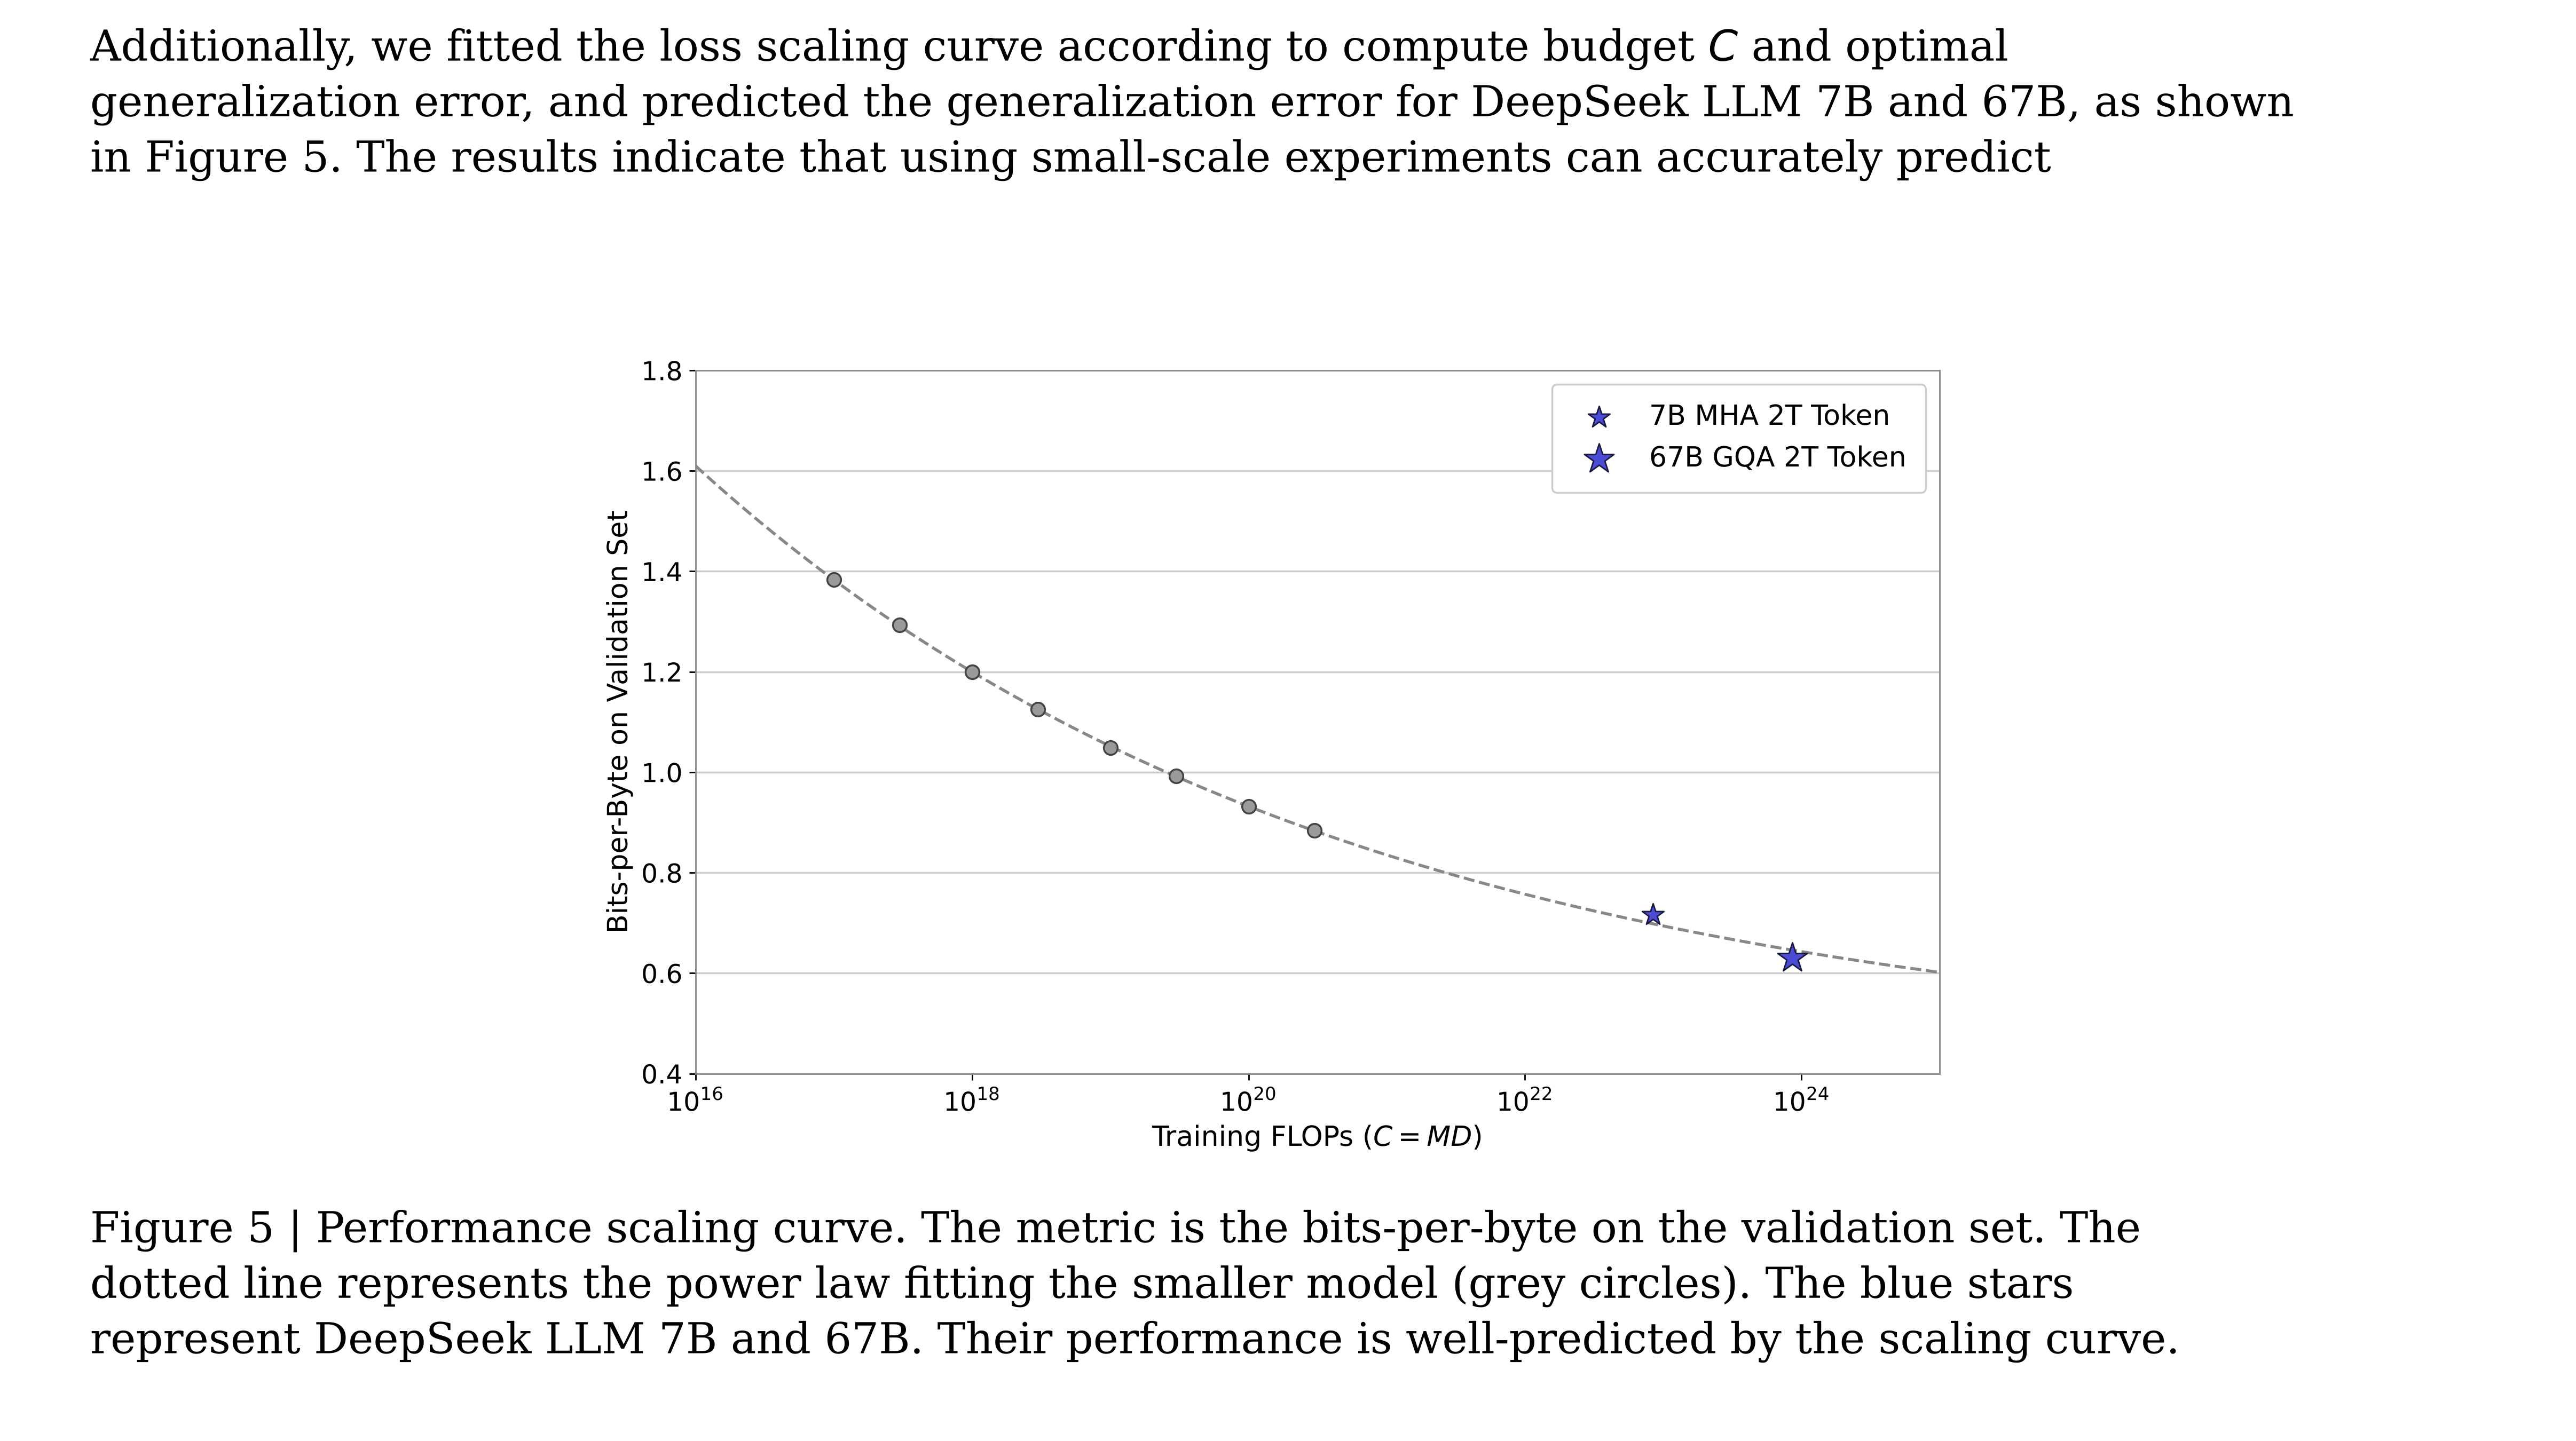
\includegraphics[width=0.8\linewidth]{figure5_hires.png}
\end{figure}

\subsubsection*{Other models: Qwen scaling}

\textbf{Qwen 2.5} - batch and hyperparameter scaling fits

\begin{center}
    We develop scaling laws for hyper-parameters based on the pre-training data of Qwen 2.5 [Hoffmann et al. (2022); Kaplan et al. (2020)]. While previous studies [Dubey et al. (2024); Almazrouei et al. (2023); Hoffmann et al. (2022)] primarily used scaling laws to determine optimal model sizes given compute budgets, we leverage them to identify optimal parameters like batch size \(B\) and learning rate \(\mu\) for both dense models and MoE models of varying sizes.
\end{center}

\begin{center}
    Through extensive experimentation, we systematically study the relationship between model architecture and optimal training hyper-parameters. Specifically, we analyze how optimal learning rate \(\mu_{\text{opt}}\) and batch size \(B_{\text{opt}}\) vary with model size \(N\) and pre-training data size \(D\). Our experiments cover a comprehensive range of architectures, including dense models with 44M to 14B parameters and MoE models with 44M to 1B activated parameters, trained on datasets ranging from 0.8B to 600B tokens. Using these optimal hyper-parameter predictions, we then model the final loss as a function of model architecture and training data scale.
\end{center}

\begin{center}
    Additionally, we leverage scaling laws to predict and compare the performance of MoE models with varying parameter counts against their dense counterparts. This analysis guides our hyper-parameter configuration for MoE models, enabling us to achieve performance parity with specific dense model variants (such as Qwen2.5-\{14,72\}B) through careful tuning of both activated and total parameters.
\end{center}

\textbf{Qwen 3} - similar for LR/batch

\begin{center}
    Similar to Qwen2.5 [Yang et al. (2024b)], we develop scaling laws for optimal hyper-parameters (e.g.\ learning rate scheduler and batch size) predictions based on three pre-training stages mentioned above. Through extensive experiments, we systematically study the relationship between model architecture, training data, training stage, and optimal training hyper-parameters. Finally, we set the predicted optimal learning rate and batch size strategy for each dense or MoE model.
\end{center}

\subsection*{Kimi K2}

Many recent papers run scaling studies to find the right sparsity level.

\begin{center}
    \textbf{Sparsity Scaling Law} We develop a sparsity scaling law tailored for Mixture-of-Experts (MoE) model family using Muon. Sparsity is defined as the ratio of the total number of experts to the number of activated experts. Through carefully controlled small-scale experiments, we observe that - under a fixed number of activated parameters (i.e.\ constant FLOPs) - increasing the total number of experts (i.e.\ increasing sparsity) consistently lowers both the training and validation loss, thereby enhancing overall model performance (Figure 5). Concretely, under the compute-optimal sparsity scaling law, achieving the same validation loss of 1.5, sparsity 48 reduces FLOPs by 1.69\(\times\), 1.39\(\times\) and 1.15\(\times\) compared to sparsity levels 8, 16 and 32, respectively. Though increasing sparsity leads to better performance, this gain comes with increased infrastructure complexity. To balance model performance with cost, we adopt a sparsity of 48 for Kimi K2, activating 8 out of 384 experts per forward pass.
\end{center}

\begin{figure}[hpbt]
    \centering
    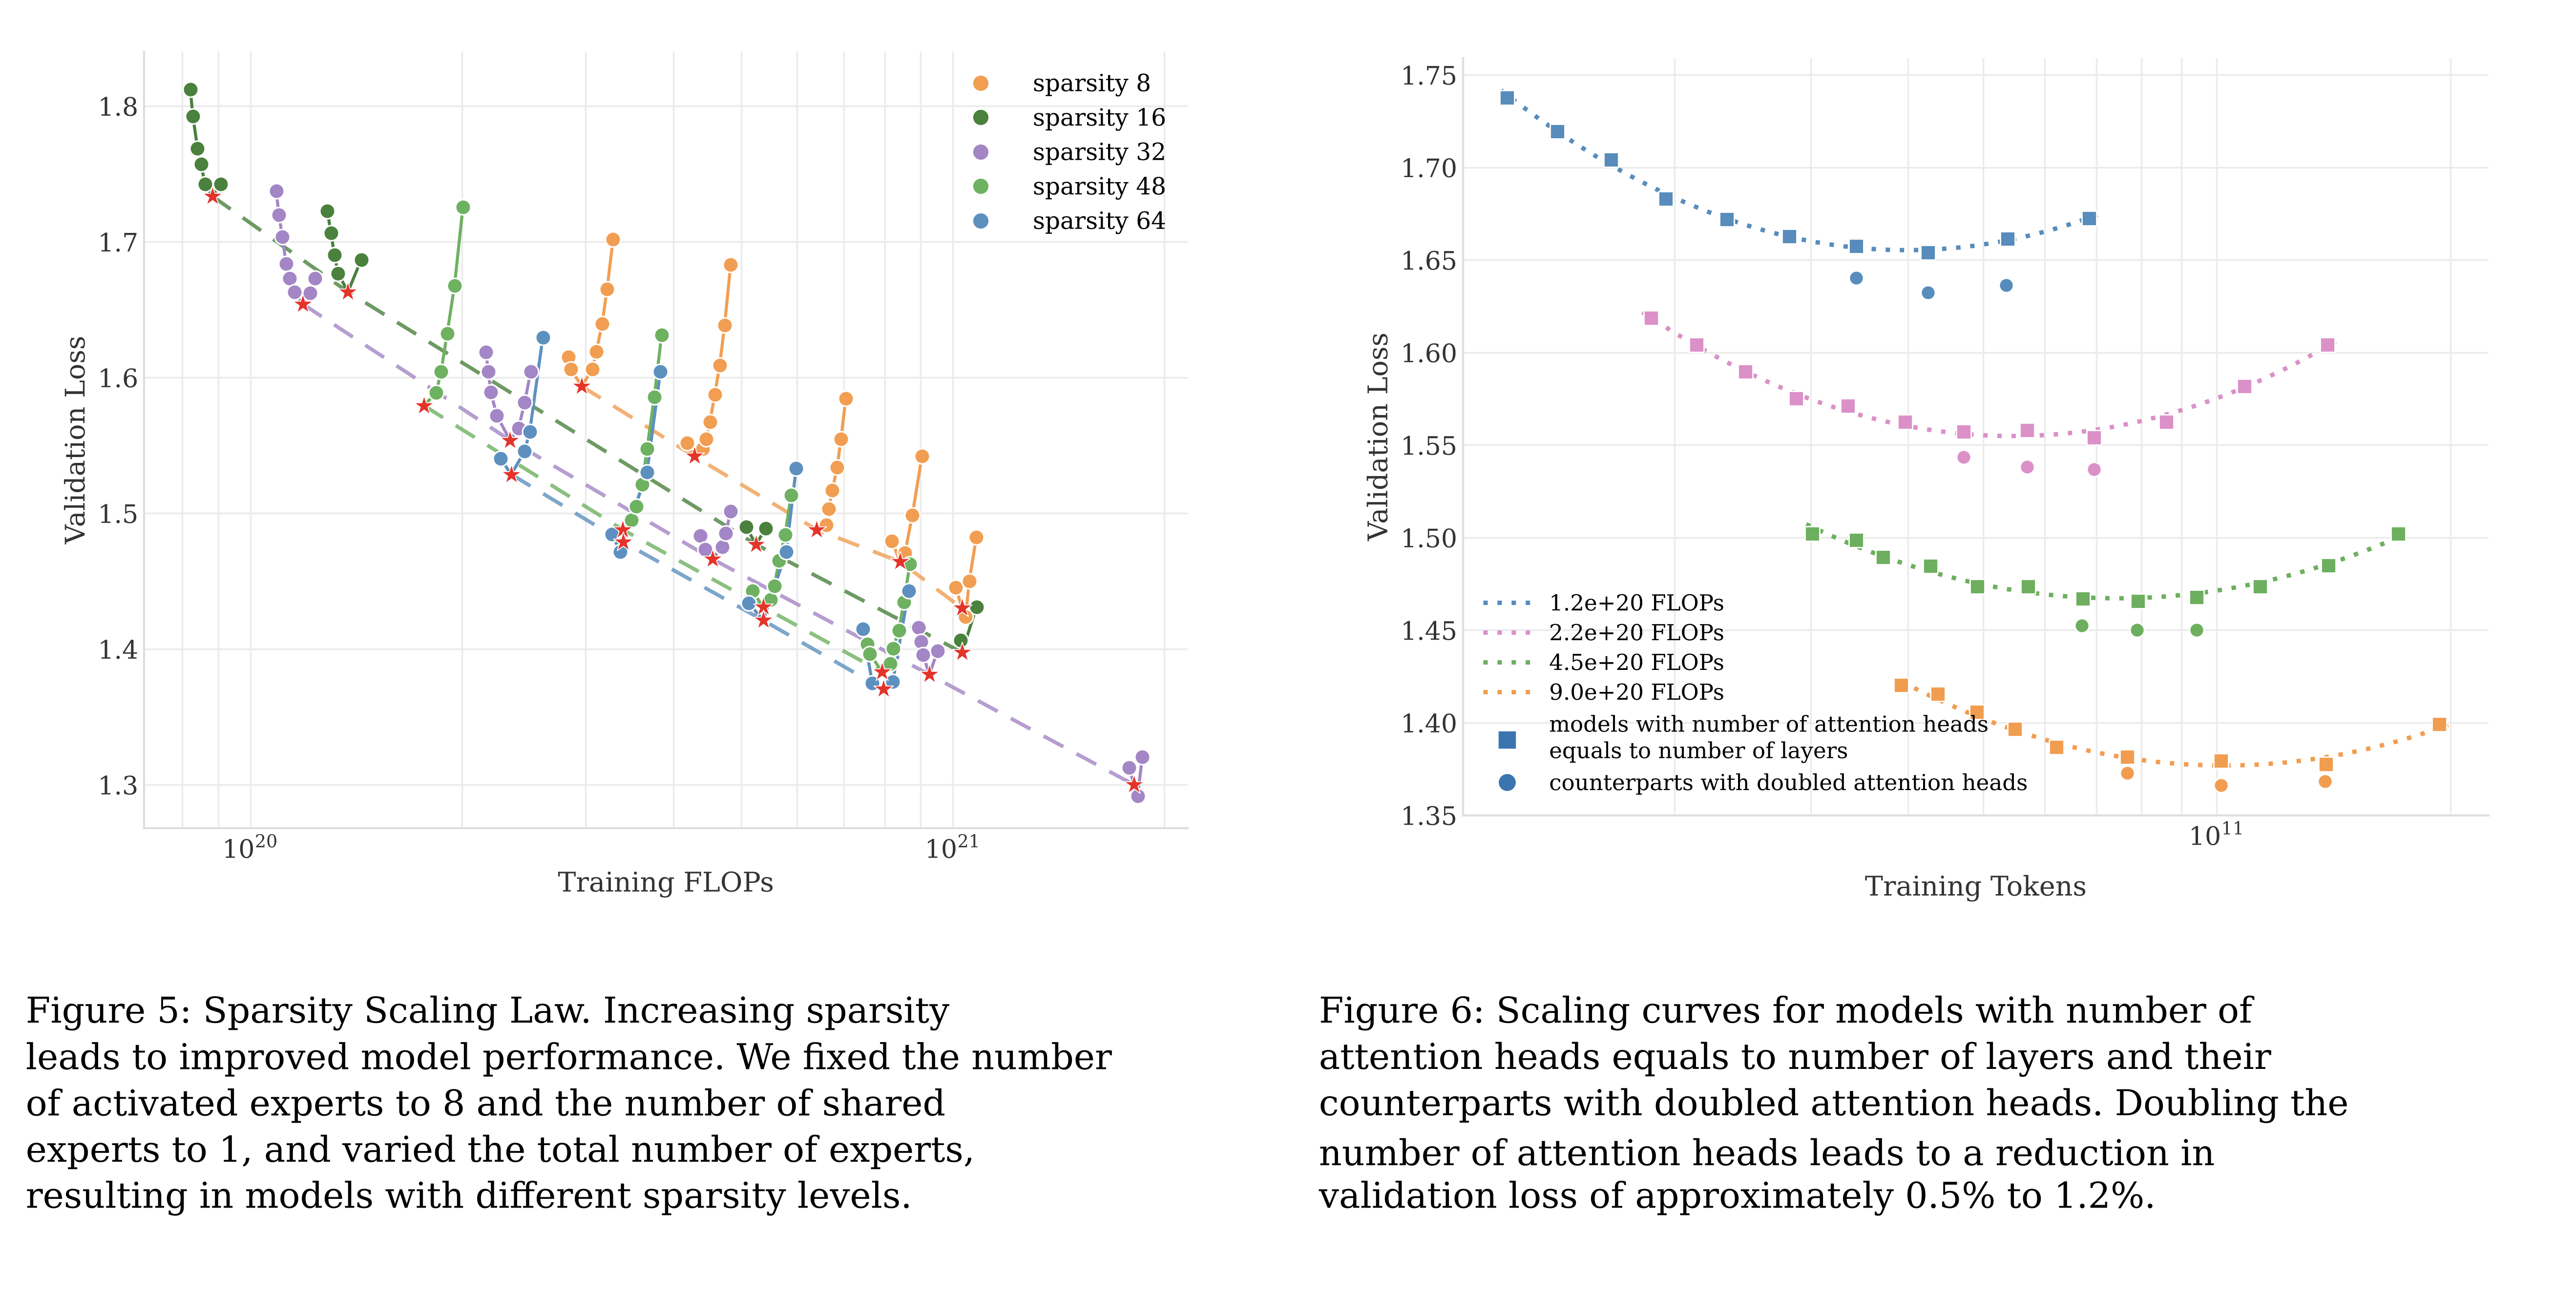
\includegraphics[width=1\linewidth]{figure5_6_hires.png}
\end{figure}

\subsubsection*{Hunyuan (2024) large scaling laws}

Yet more IsoFLOP-style scaling (but this time for MoE parameter sizes).

\begin{figure}[hpbt]
    \centering
    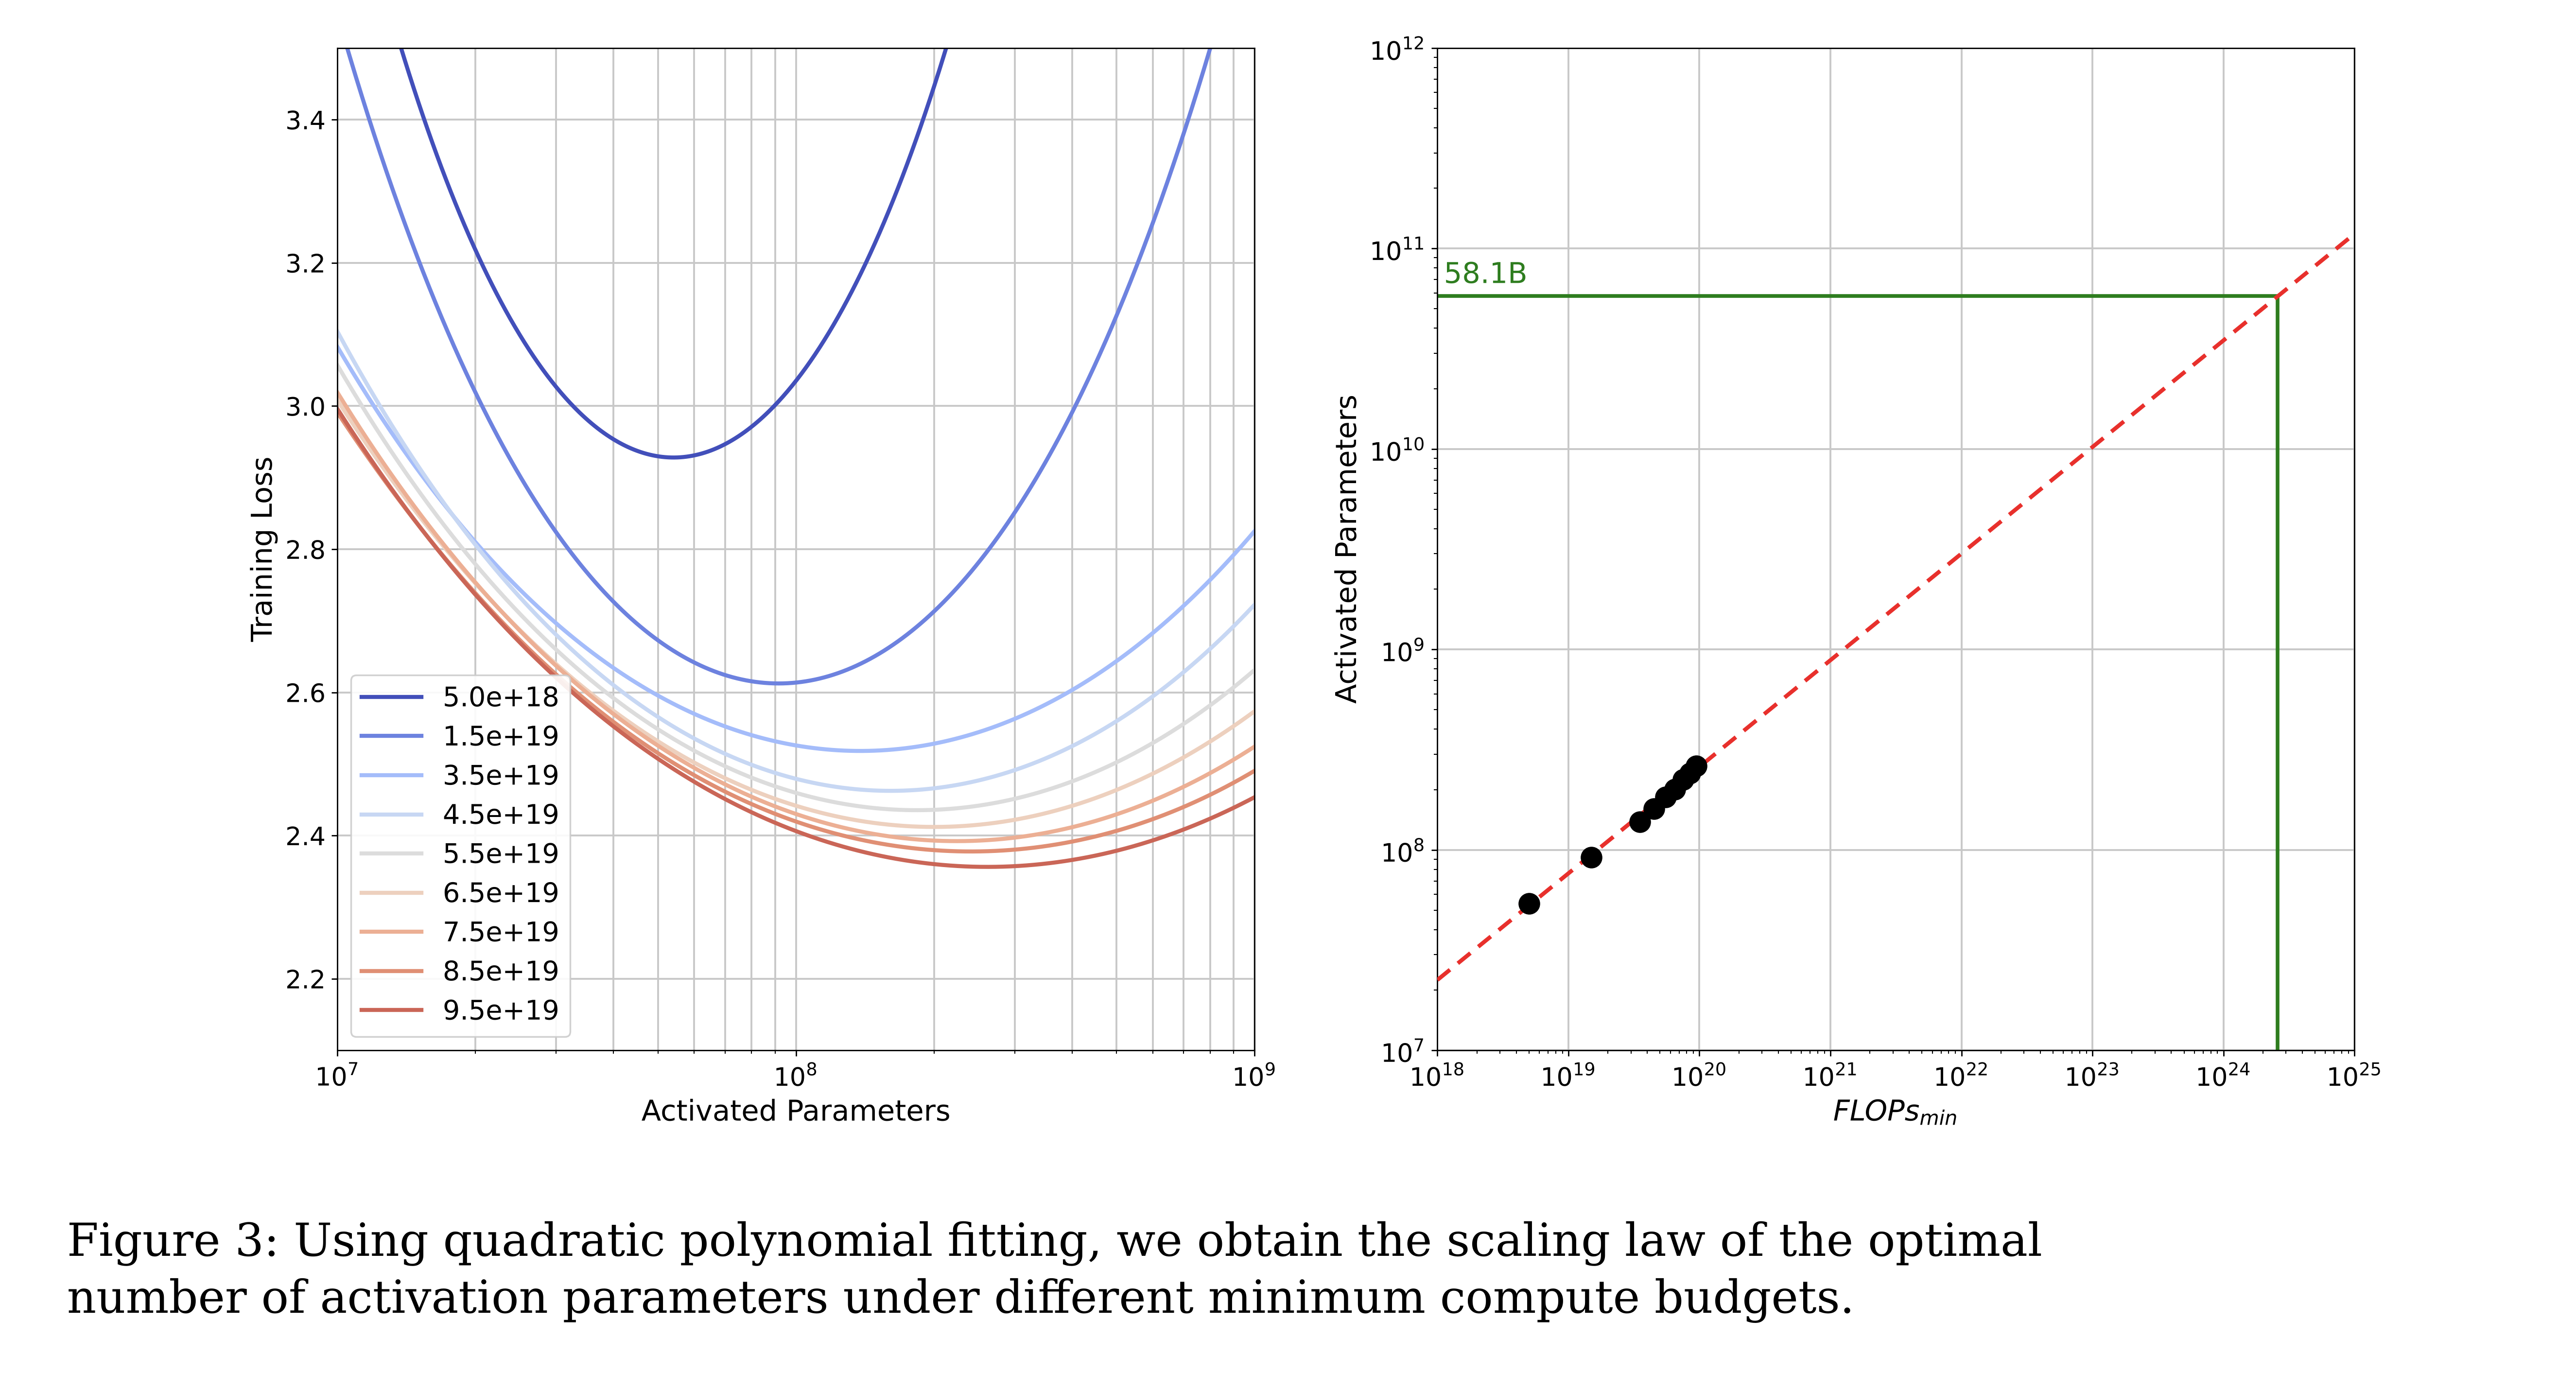
\includegraphics[width=0.75\linewidth]{figure3_activated_hires.png}
\end{figure}

\begin{center}
    Optimal ratio: 96-1 (data to active param)
\end{center}

\subsubsection*{LLaMA 3 (2024) scaling laws}

\begin{figure}[hpbt]
    \centering
    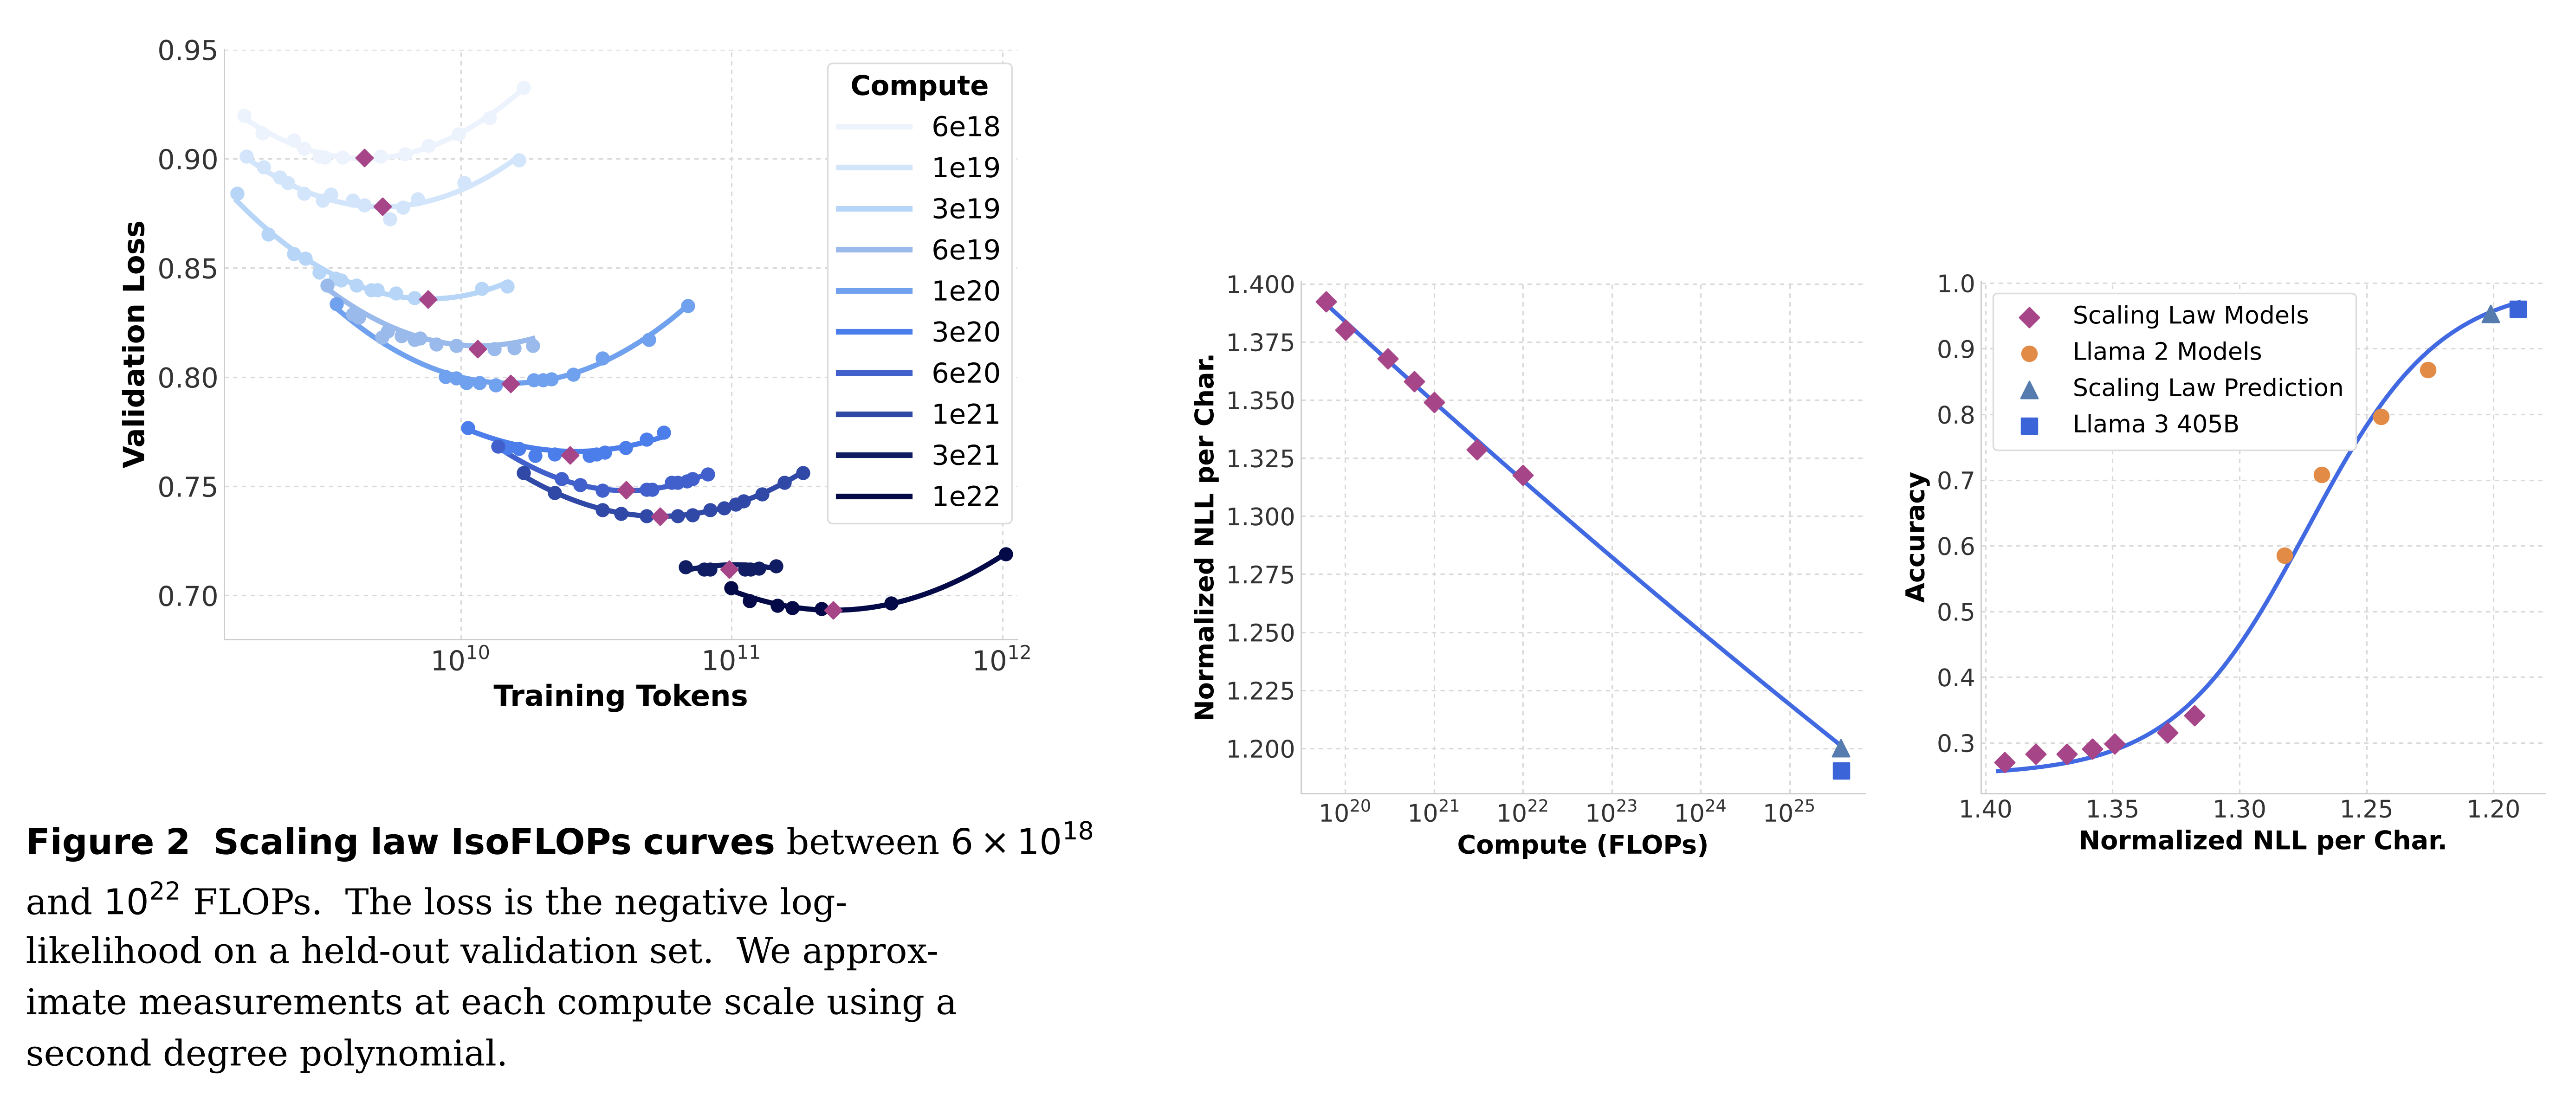
\includegraphics[width=1\linewidth]{figure2_isoflops_hires.png}
\end{figure}

IsoFLOPs-style scaling (39-1 ratio) \hfill Compute-to-downstream scaling

\subsubsection*{MiniMax-01 (2025)}

Architecture scaling laws

\begin{figure}[hpbt]
    \centering
    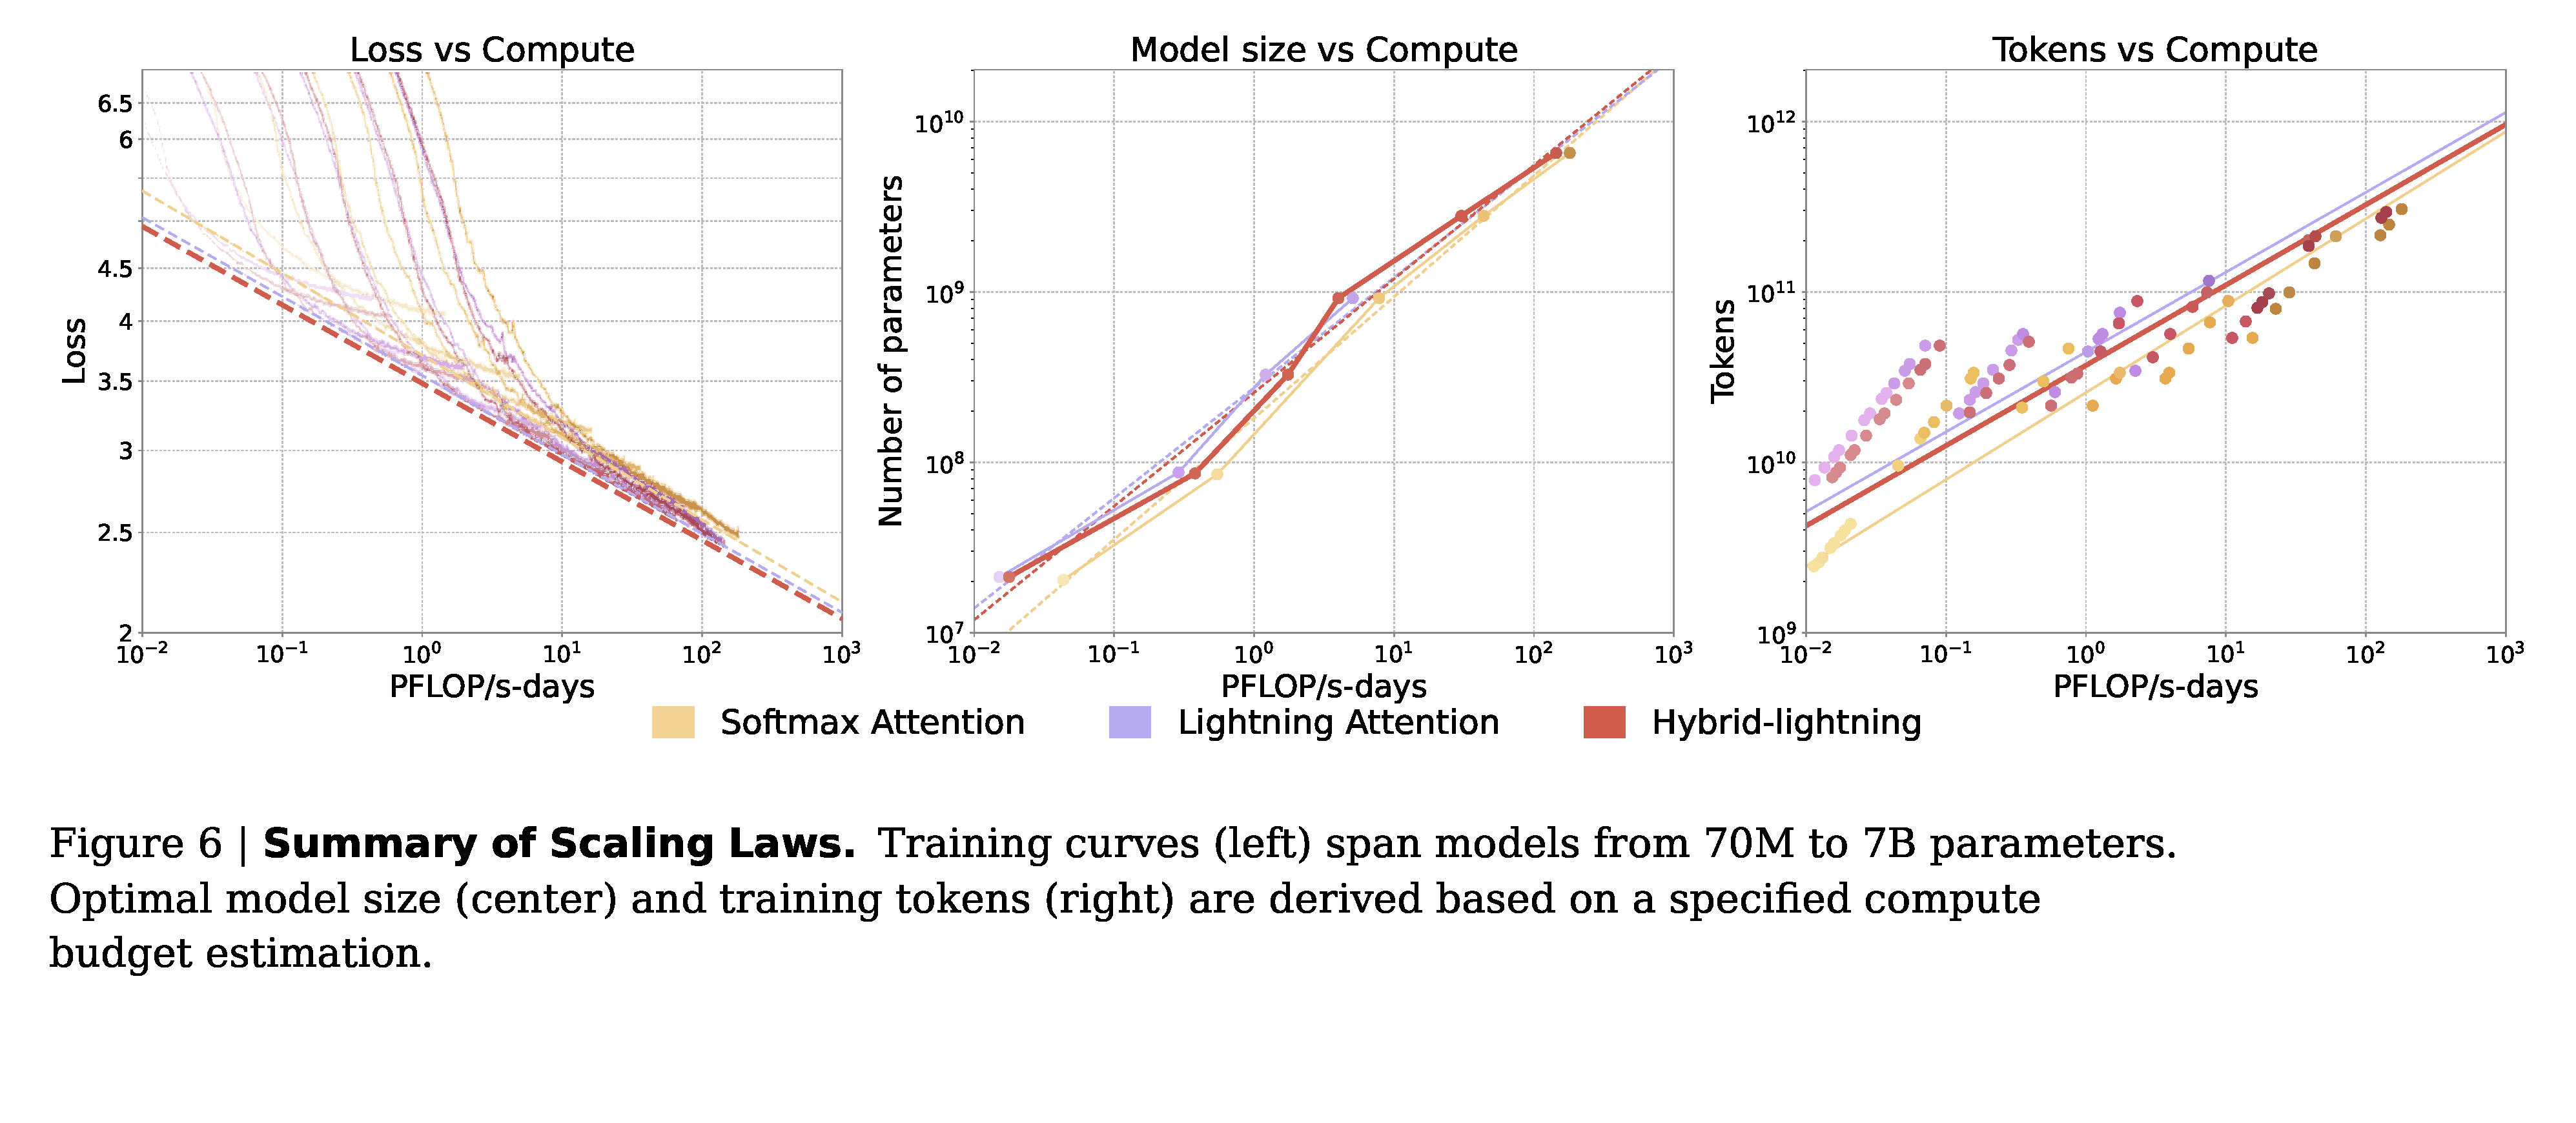
\includegraphics[width=1\linewidth]{figure6_scaling_summary_hires.pdf}
\end{figure}

Chinchilla first method

\subsection*{Recent scaling law recipes}

\textbf{miniCPM recipe}

\begin{itemize}
    \item Use muP to make transformer \(+\) LR invariant to scale
    \item Use a piecewise linear schedule to get samples for Chinchilla third method (curve fitting)
\end{itemize}

\textbf{DeepSeek recipe}

\begin{itemize}
    \item Assume most transformer hypers are invariant to scale
    \item Do a scaling analysis on batch / LR to figure out optimal scaling
    \item IsoFLOP analysis to figure out model sizing
\end{itemize}

\begin{center}
    Use a piecewise-linear schedule to make Chinchilla scaling cheap.
\end{center}

\textbf{Kimi K2 recipe}
\begin{itemize}
    \item Sparsity scaling law (with Muon): at fixed activated parameters, sweep total experts to pick the sparsity level
\end{itemize}

\textbf{Other recipes}
\begin{itemize}
    \item \textbf{Qwen} - LR / batch (very few details\ldots)
    \item \textbf{LLaMA 3 / Hunyuan} - Just IsoFLOPs (no other scaling details)
    \item \textbf{MiniMax}: Architecture choice / decision scaling
\end{itemize}

\subsection*{Optimizer scaling}

Optimizer choices / tuning can be tricky and scale sensitive.

\begin{figure}[hpbt]
    \centering
    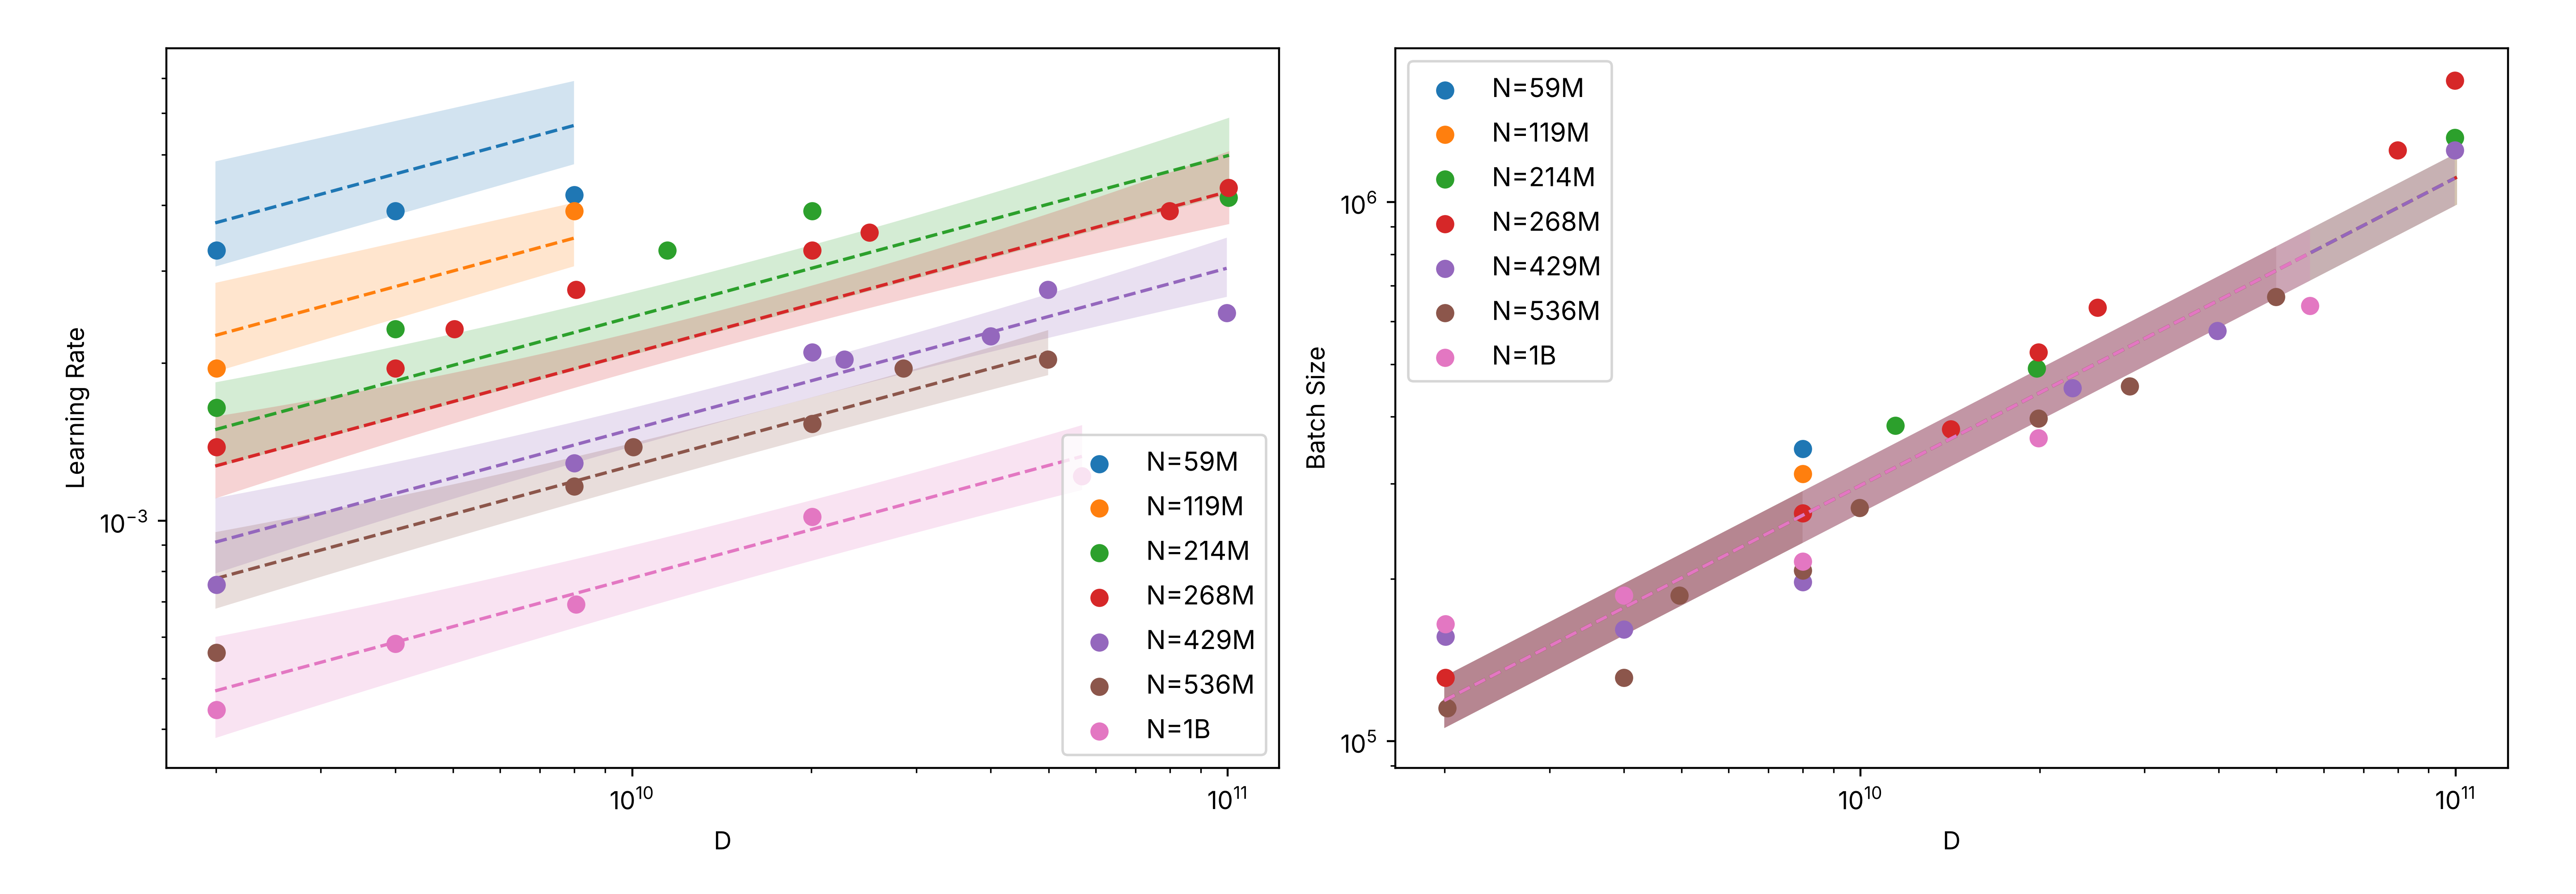
\includegraphics[width=1\linewidth]{figure_lr_bs_hires.png}
\end{figure}

How should we pick different optimizers?

\begin{figure}[hpbt]
    \centering
    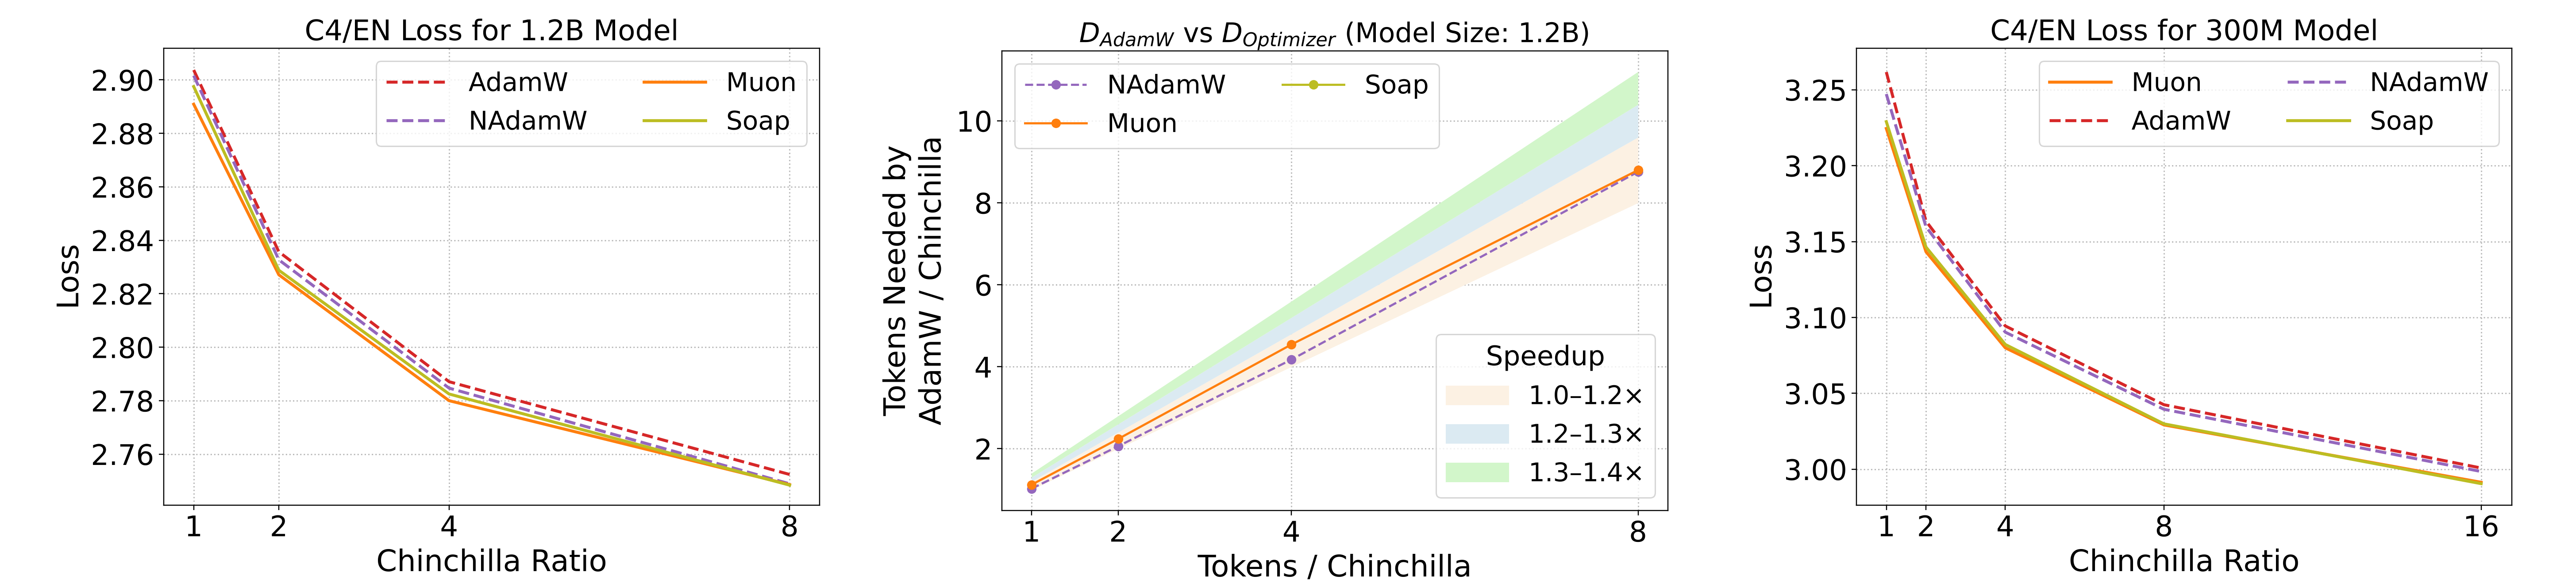
\includegraphics[width=1\linewidth]{figure_optimizers_hires.png}
\end{figure}

\subsubsection*{StepFun scaling law study}

Large-scale scaling law study from StepFun.

\begin{figure}[H]
    \centering
    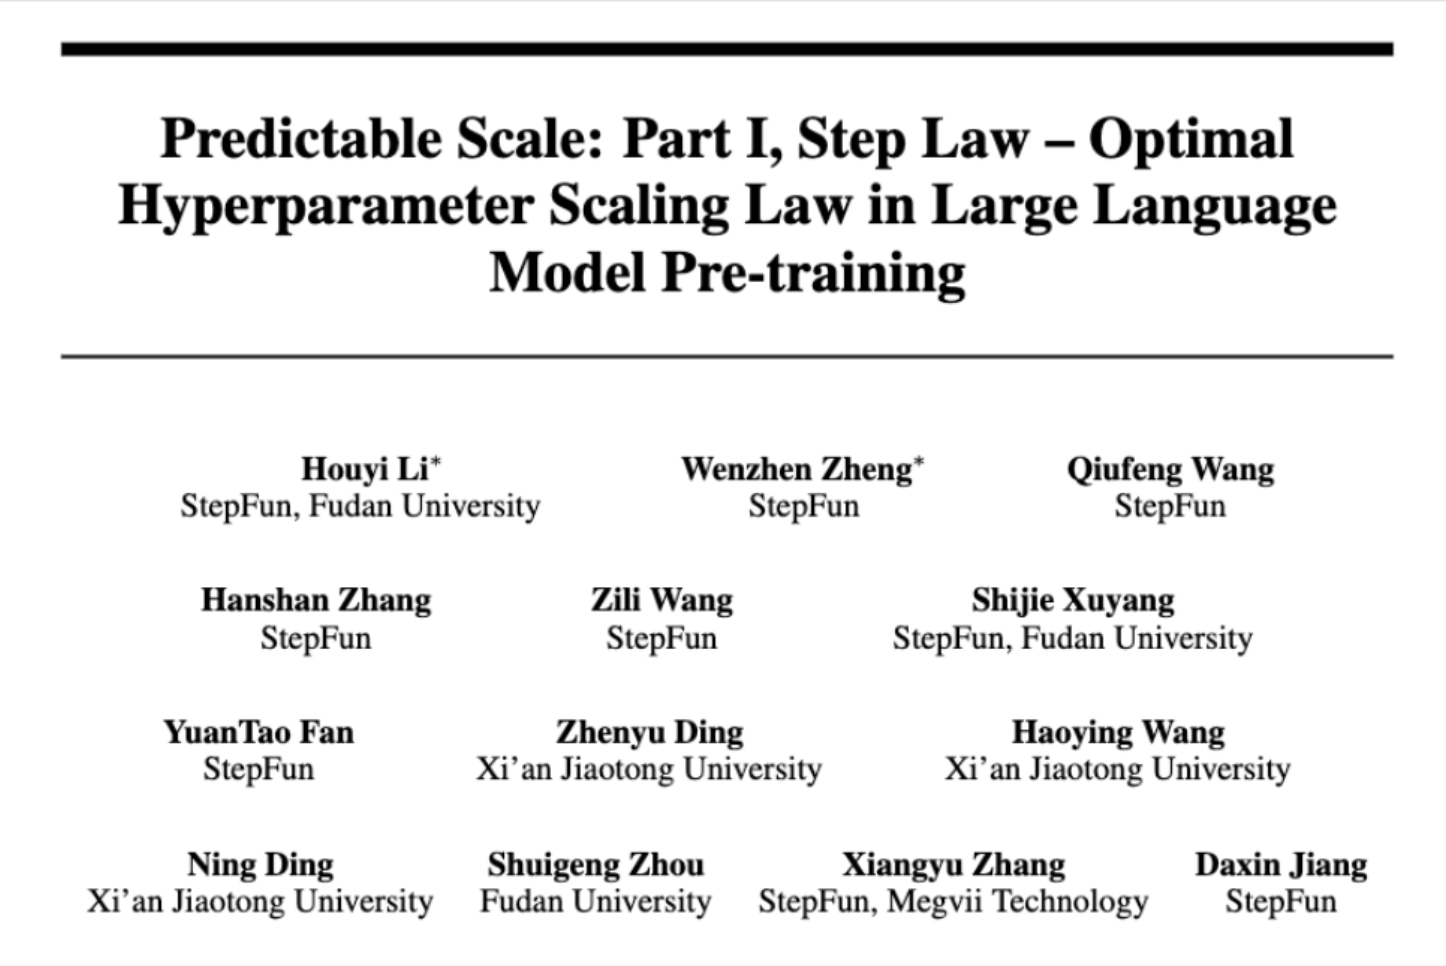
\includegraphics[width=0.8\linewidth]{StepFun.png}
\end{figure}

\begin{center}
    \textbf{Core question}: how do we set LR / batch params as we scale? (DeepSeek / Qwen approach)
\end{center}

What are the right variables / functional form?

\begin{figure}[hpbt]
    \centering
    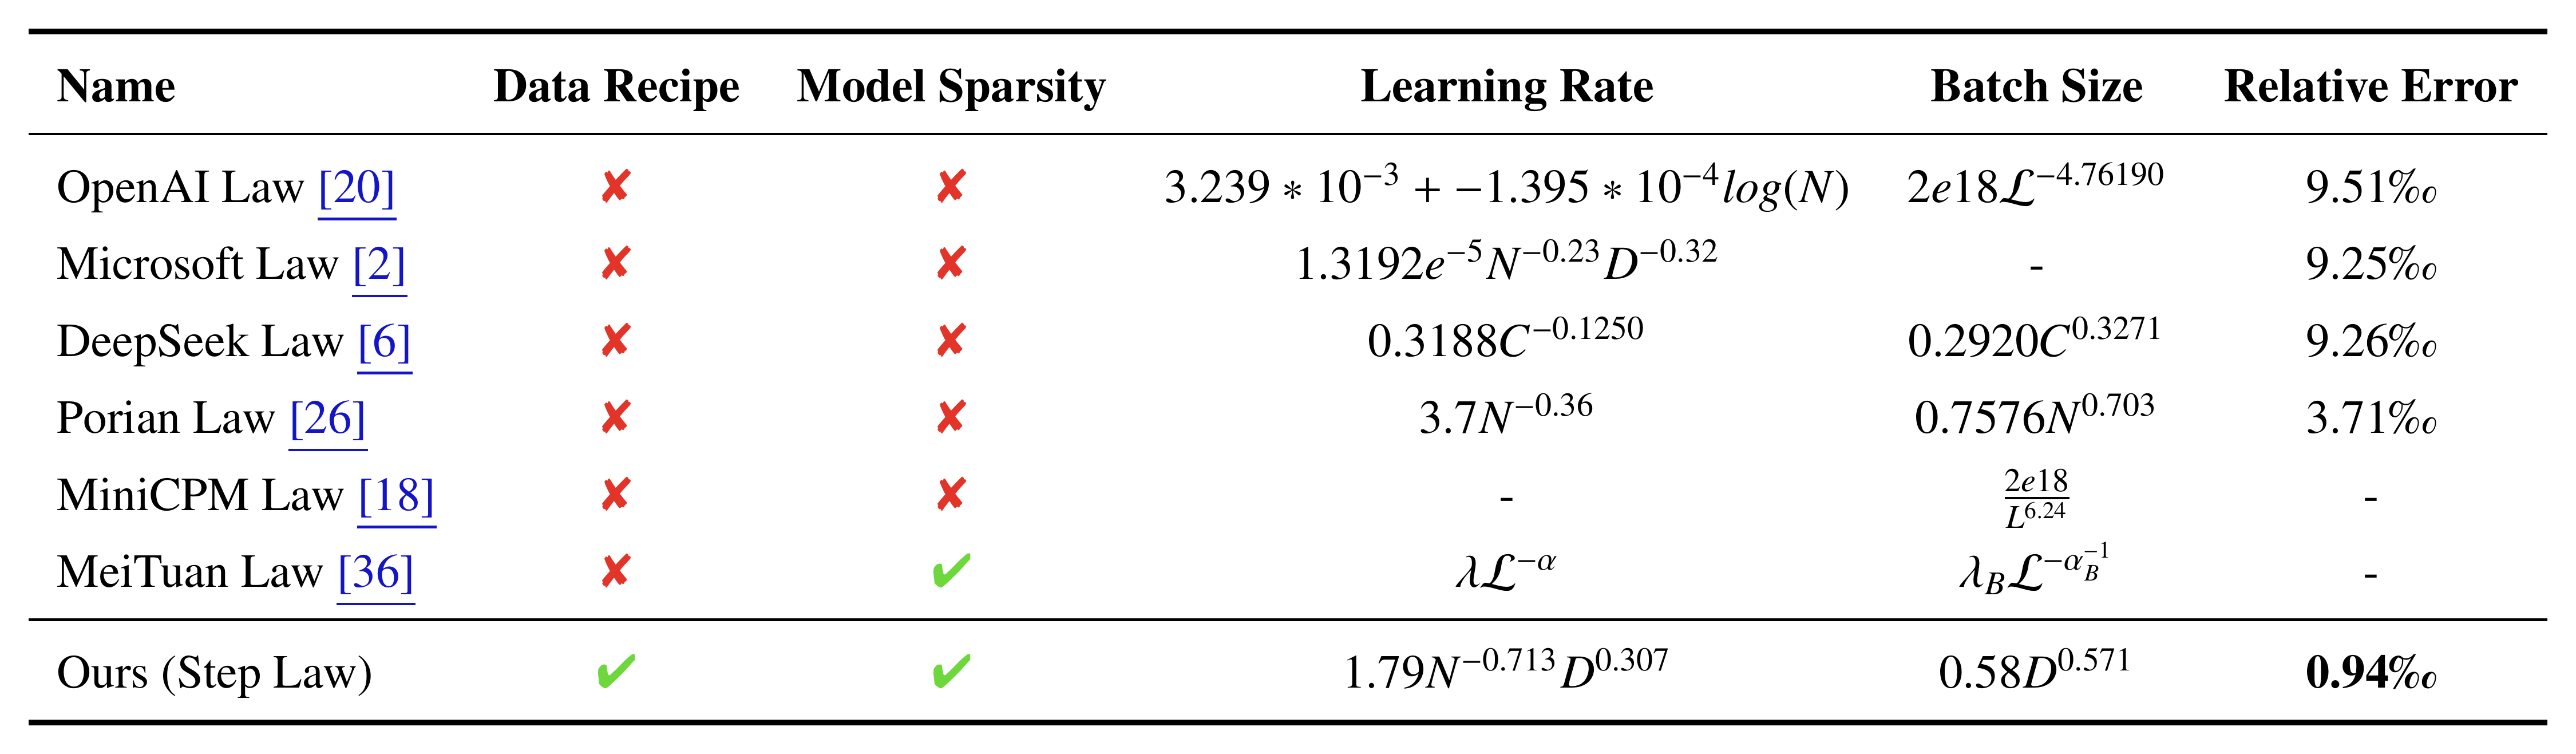
\includegraphics[width=0.8\linewidth]{table.png}
\end{figure}

\textbf{Different views}:
\begin{itemize}
    \item Critical batch: batch as a function of loss (OpenAI)
    \item Compute power law: polynomial function of compute (DeepSeek)
    \item Or something else?
\end{itemize}

\subsubsection*{The approach: purely empirical - grid search the space}

Much like the DeepSeek paper - train models to try to map out the hparam space.

\begin{figure}[hpbt]
    \centering
    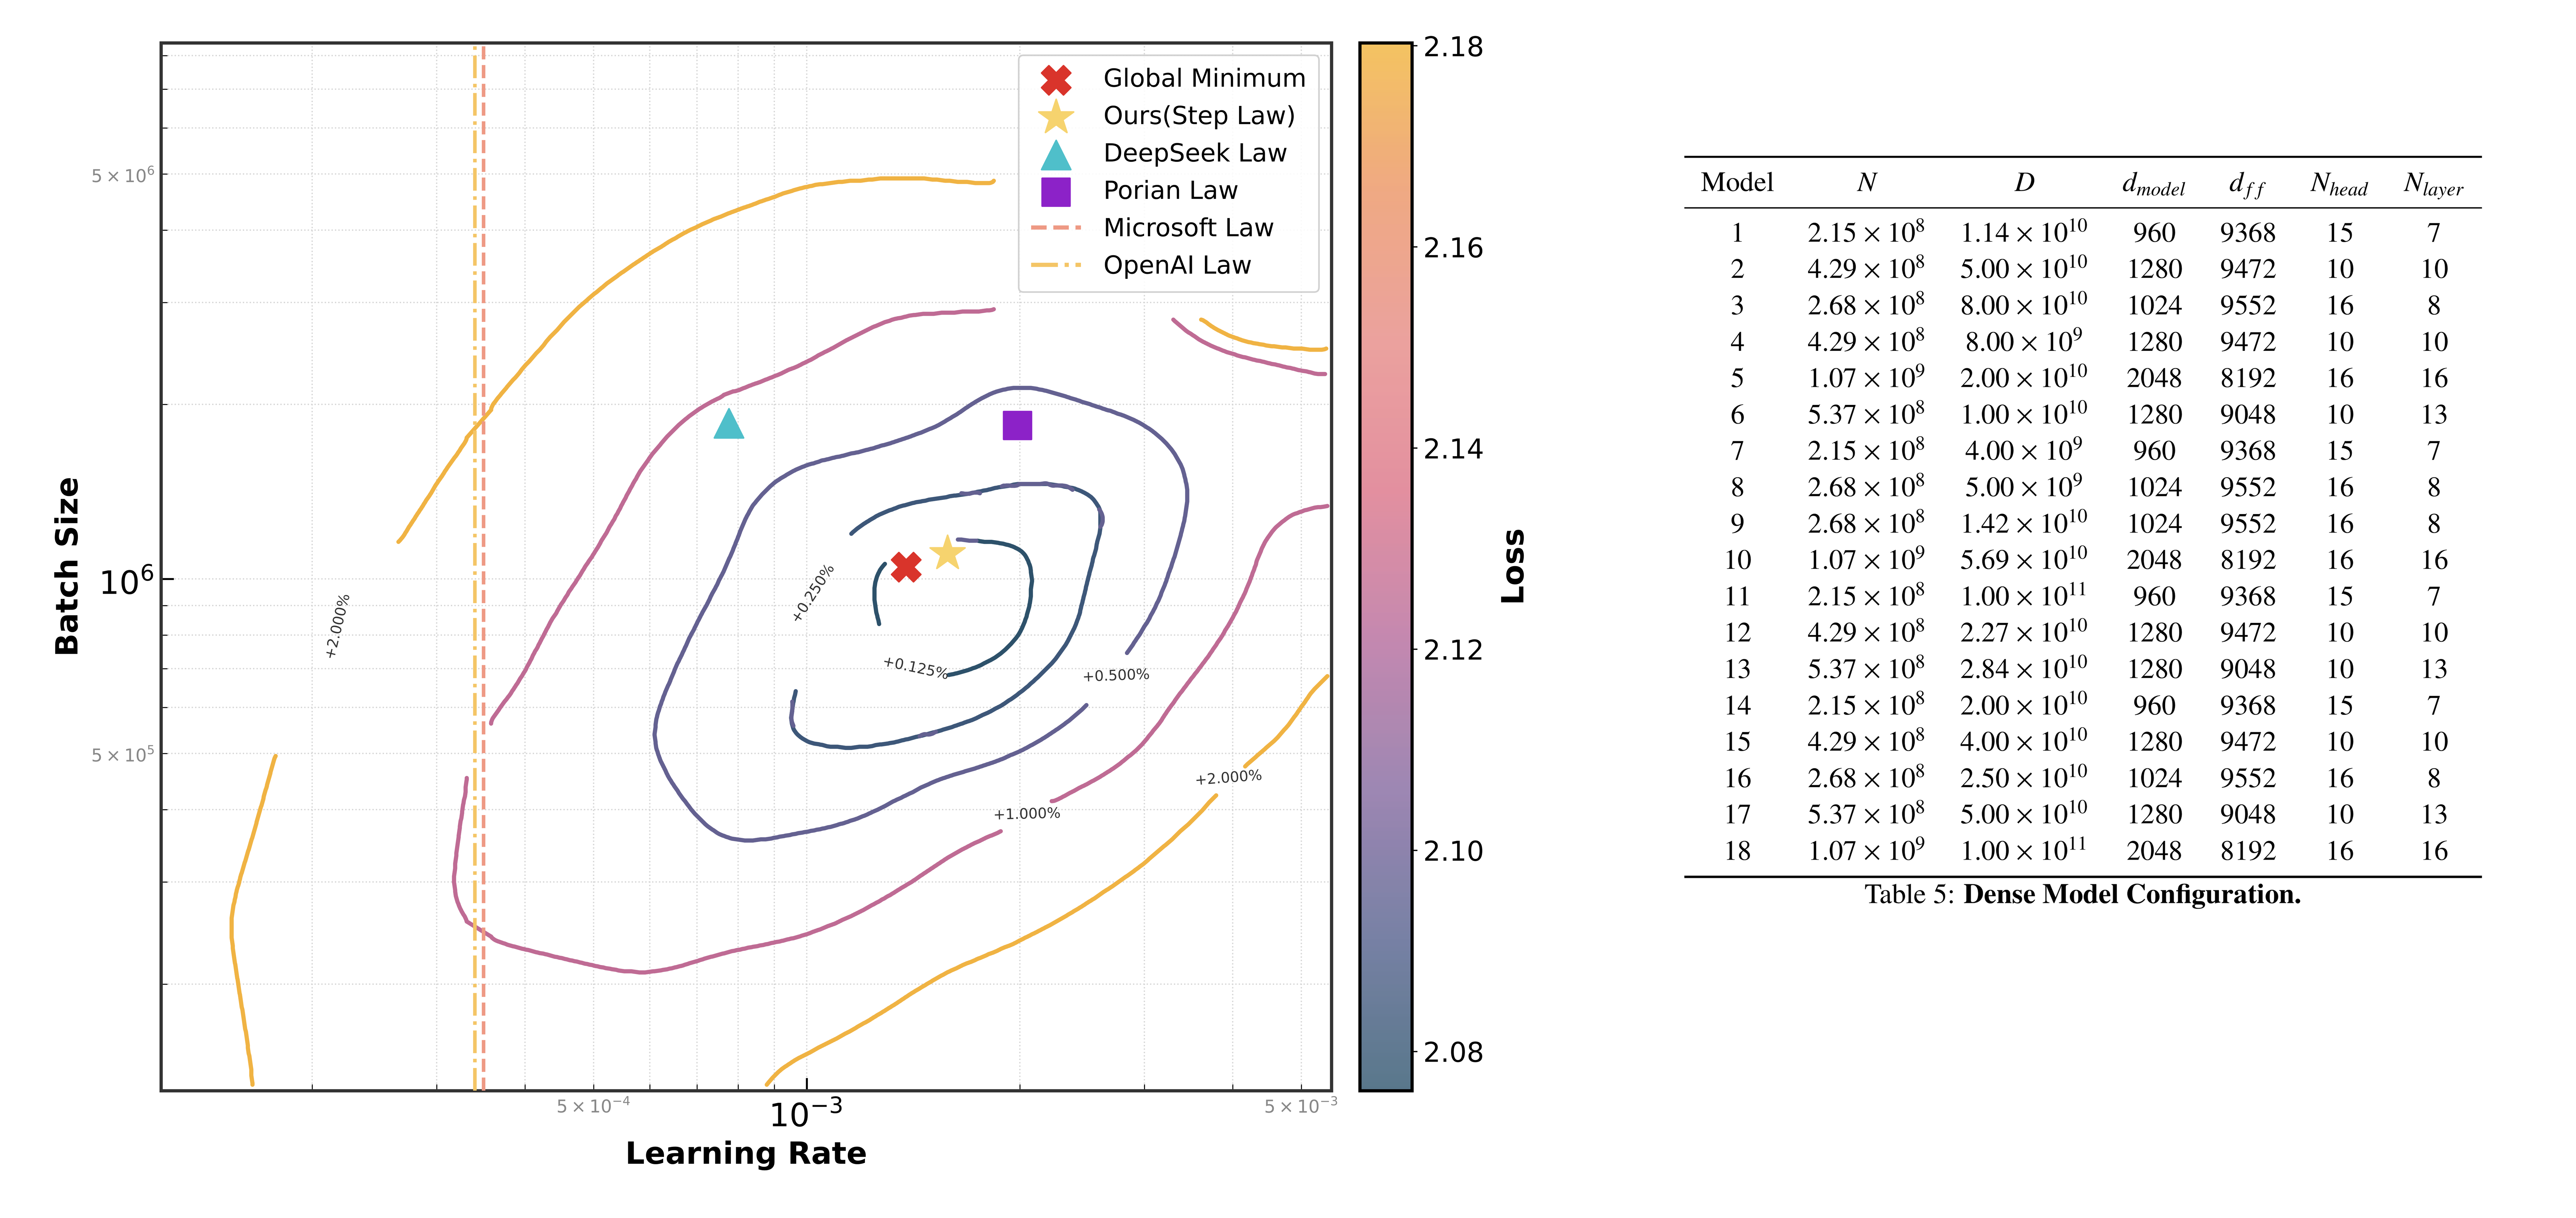
\includegraphics[width=0.8\linewidth]{figure_contour_table5_combined.png}
\end{figure}

\subsubsection*{Observation 1: loss over batch / LR is convex}

\begin{figure}[hpbt]
    \centering
    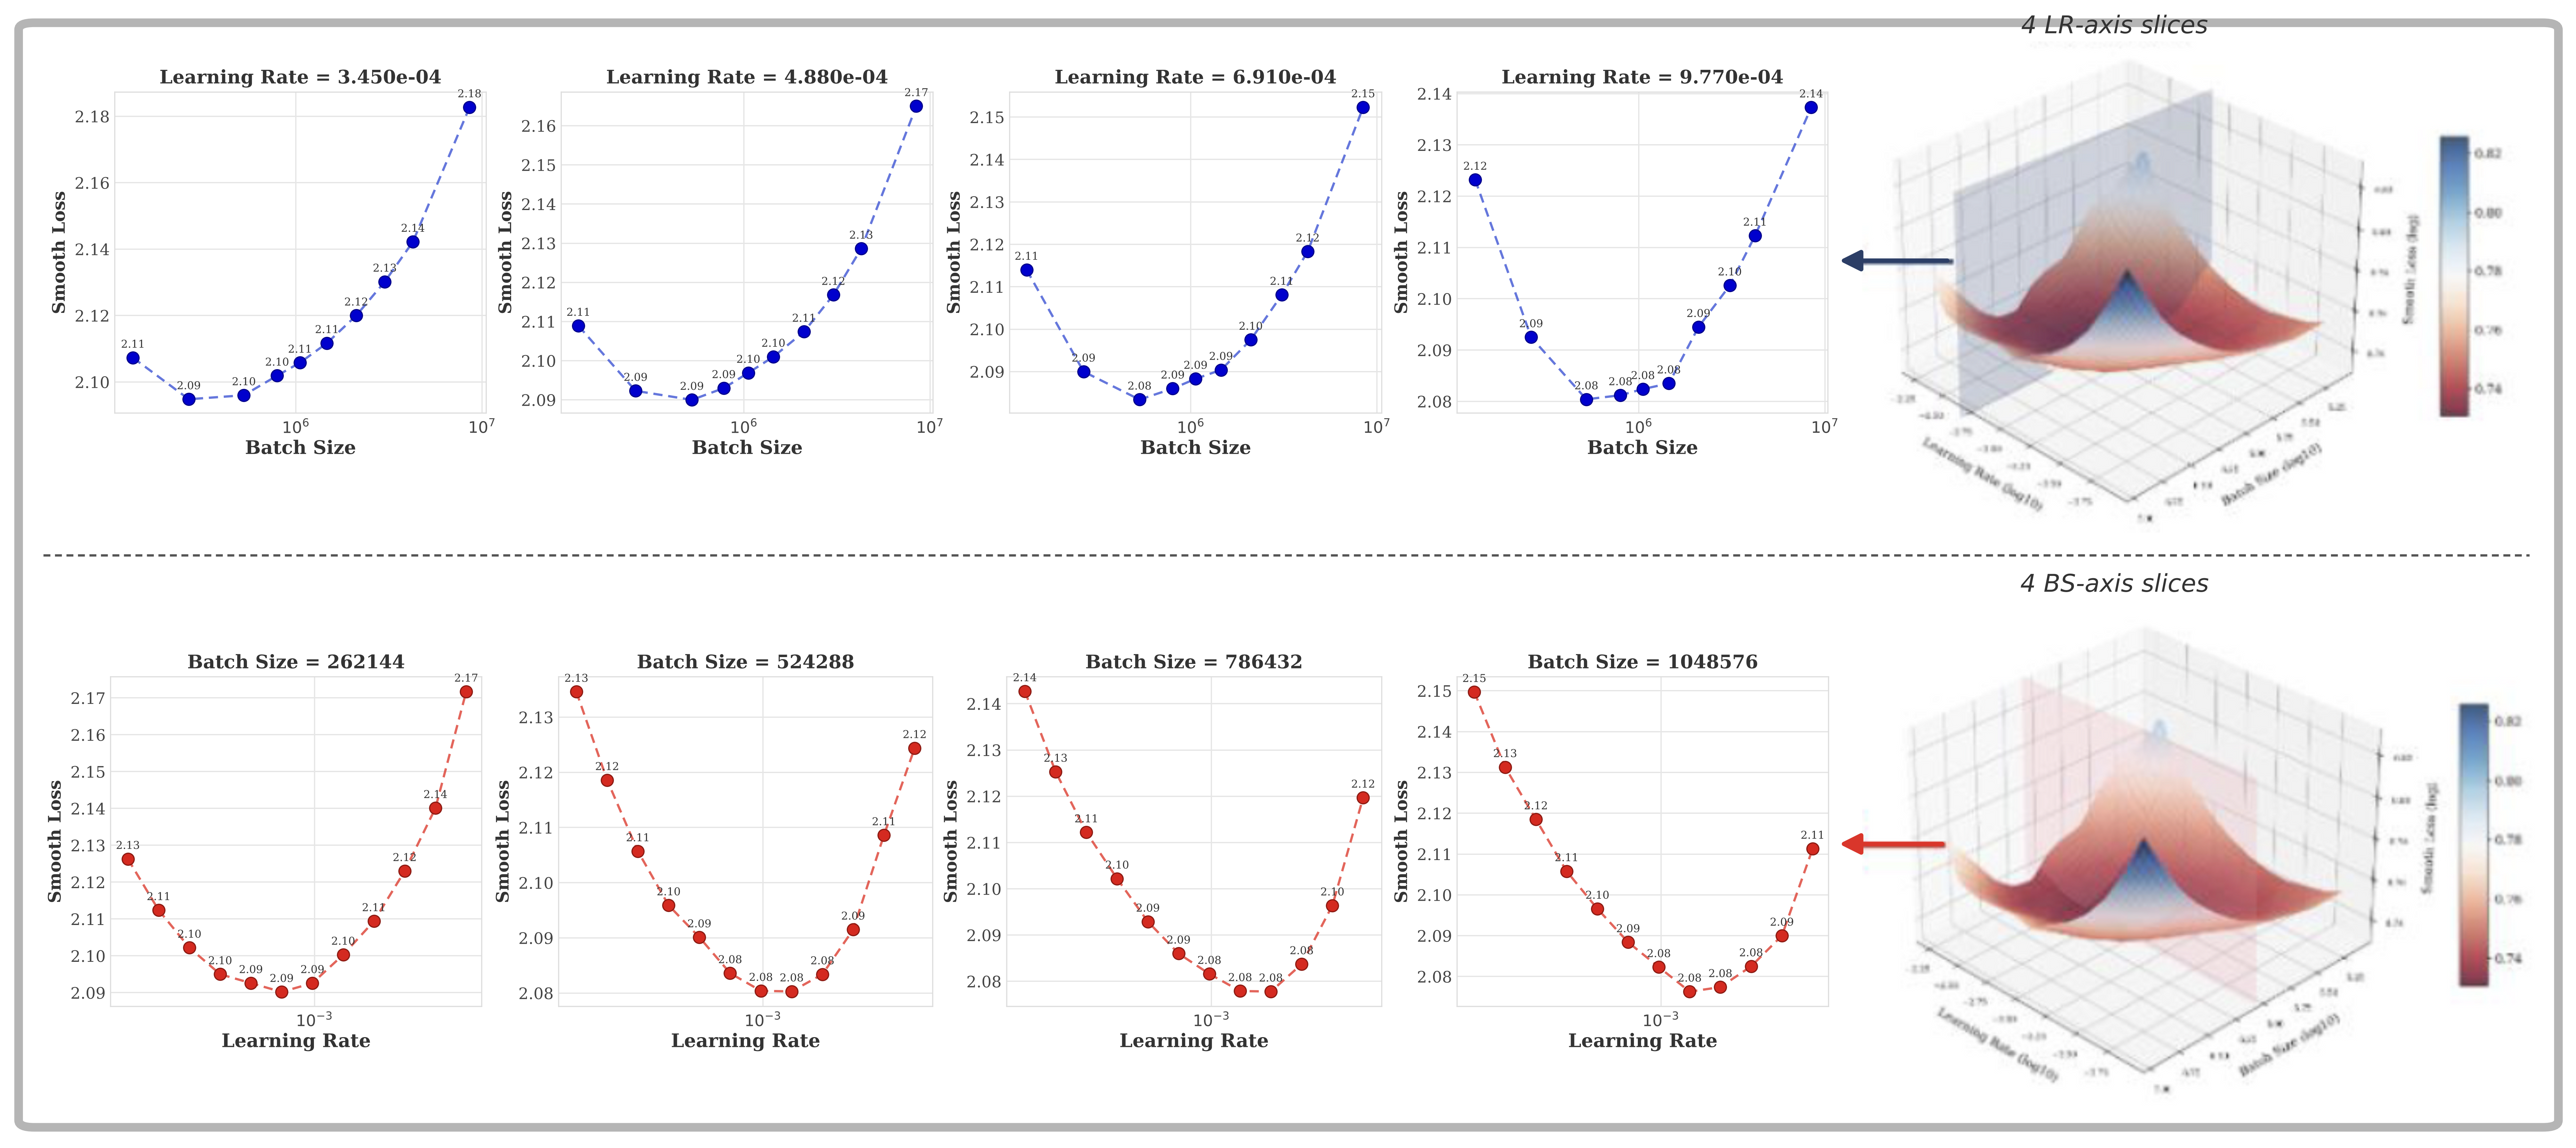
\includegraphics[width=1\linewidth]{figure_slices_hires.png}
\end{figure}

\begin{center}
    For pre-training losses, minimizers for LR / batch can be cleanly identified.
\end{center}

\subsubsection*{Observation 2: scaling trends}

\begin{figure}[hpbt]
    \centering
    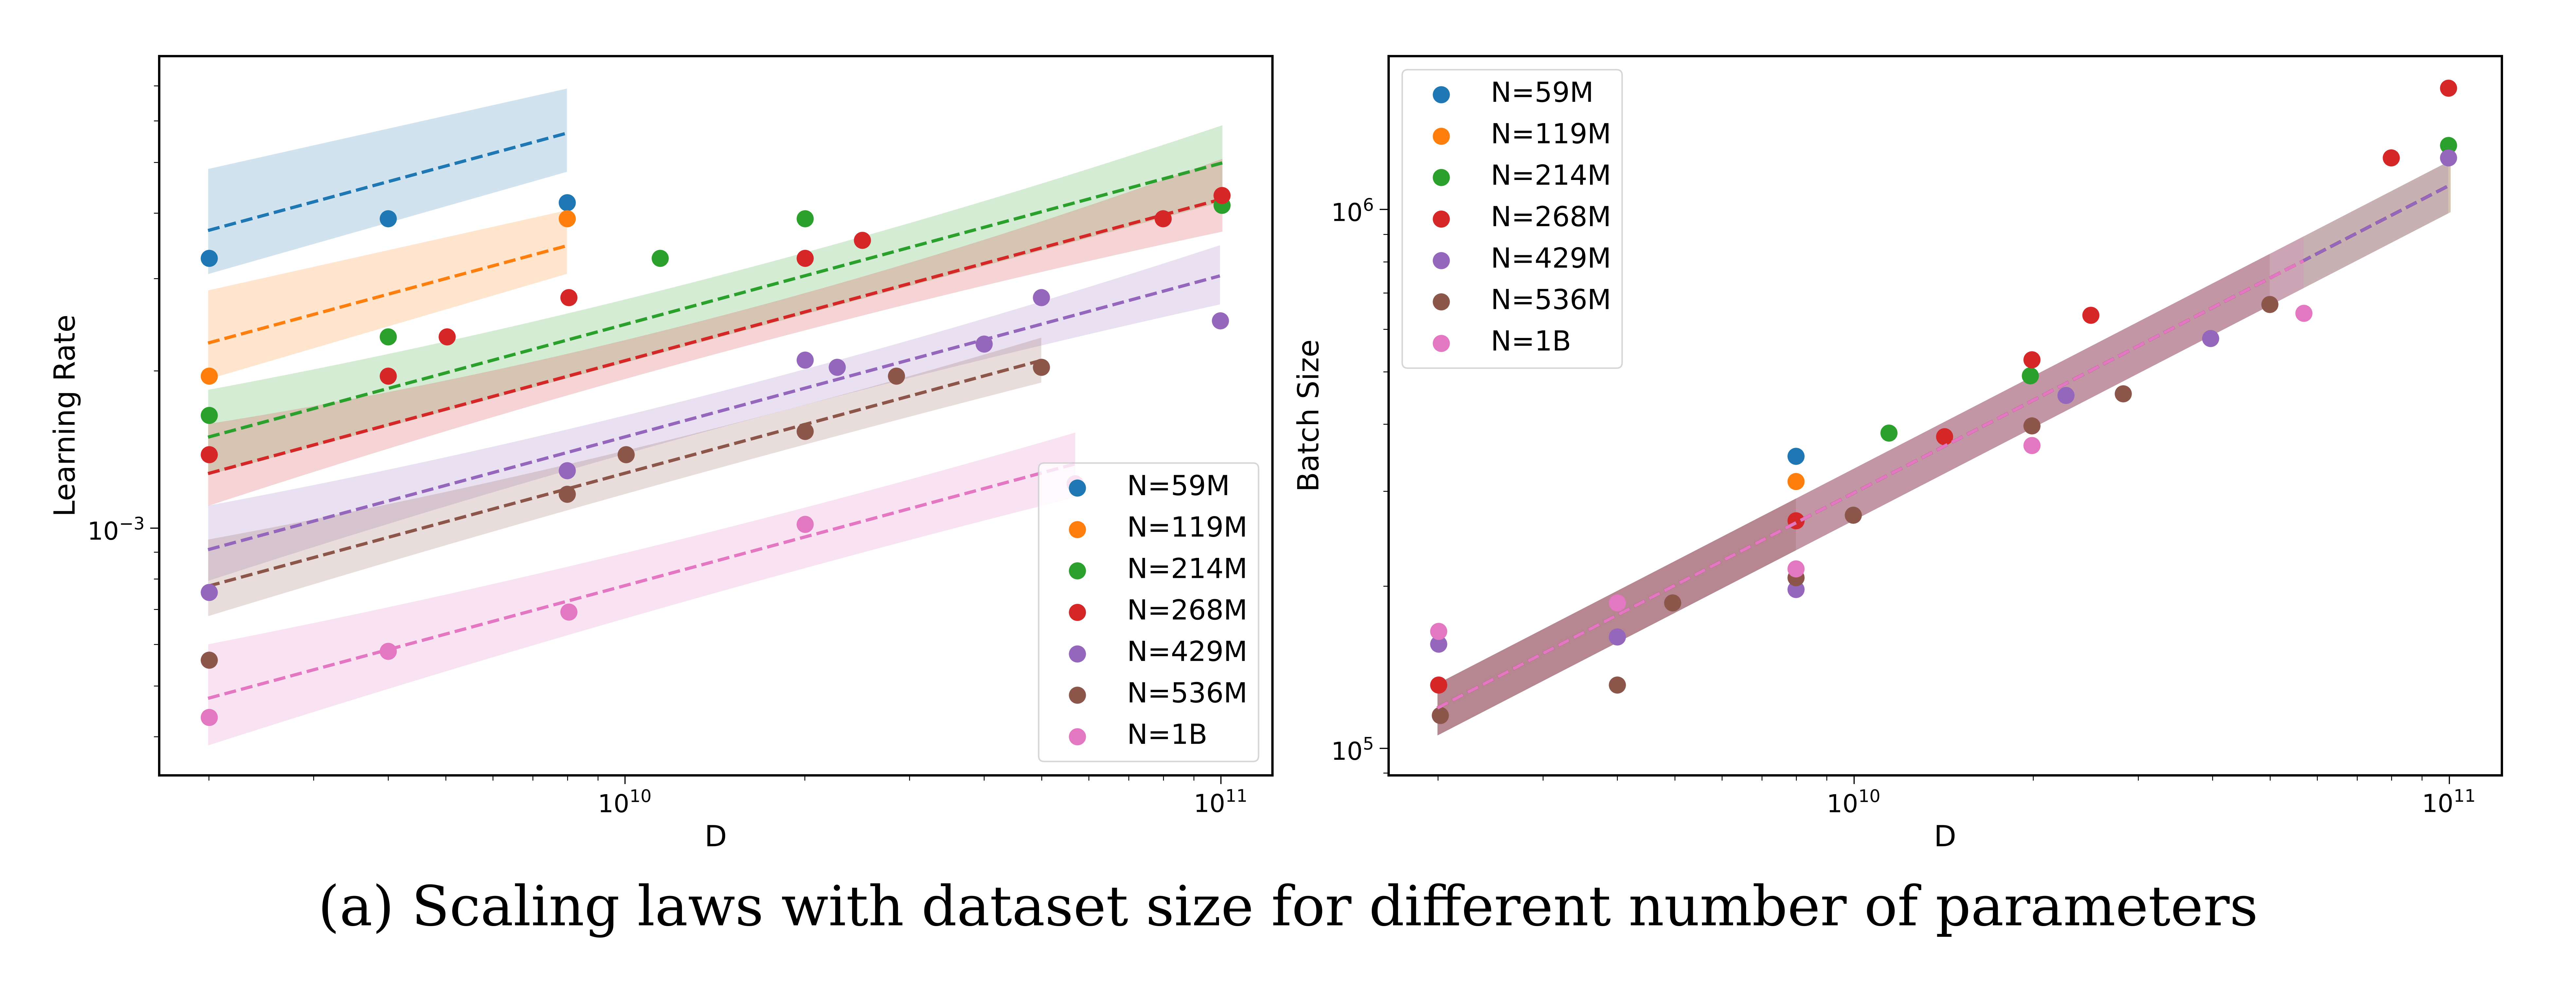
\includegraphics[width=1\linewidth]{figure_a_scaling_dataset_hires.png}
\end{figure}

\textbf{For Chinchilla-style joint scaling}: batch is primarily dependent on dataset size.

\begin{center}
    They also find higher optimal LR with D (for fixed M), but this is likely more fragile if swapping to WSD - see e.g.\ InternLM scaling law paper (Zhou+ 2026).
\end{center}

\subsubsection*{Observation 3: robustness?}

Generalization to MoEs!

\begin{figure}[hpbt]
    \centering
    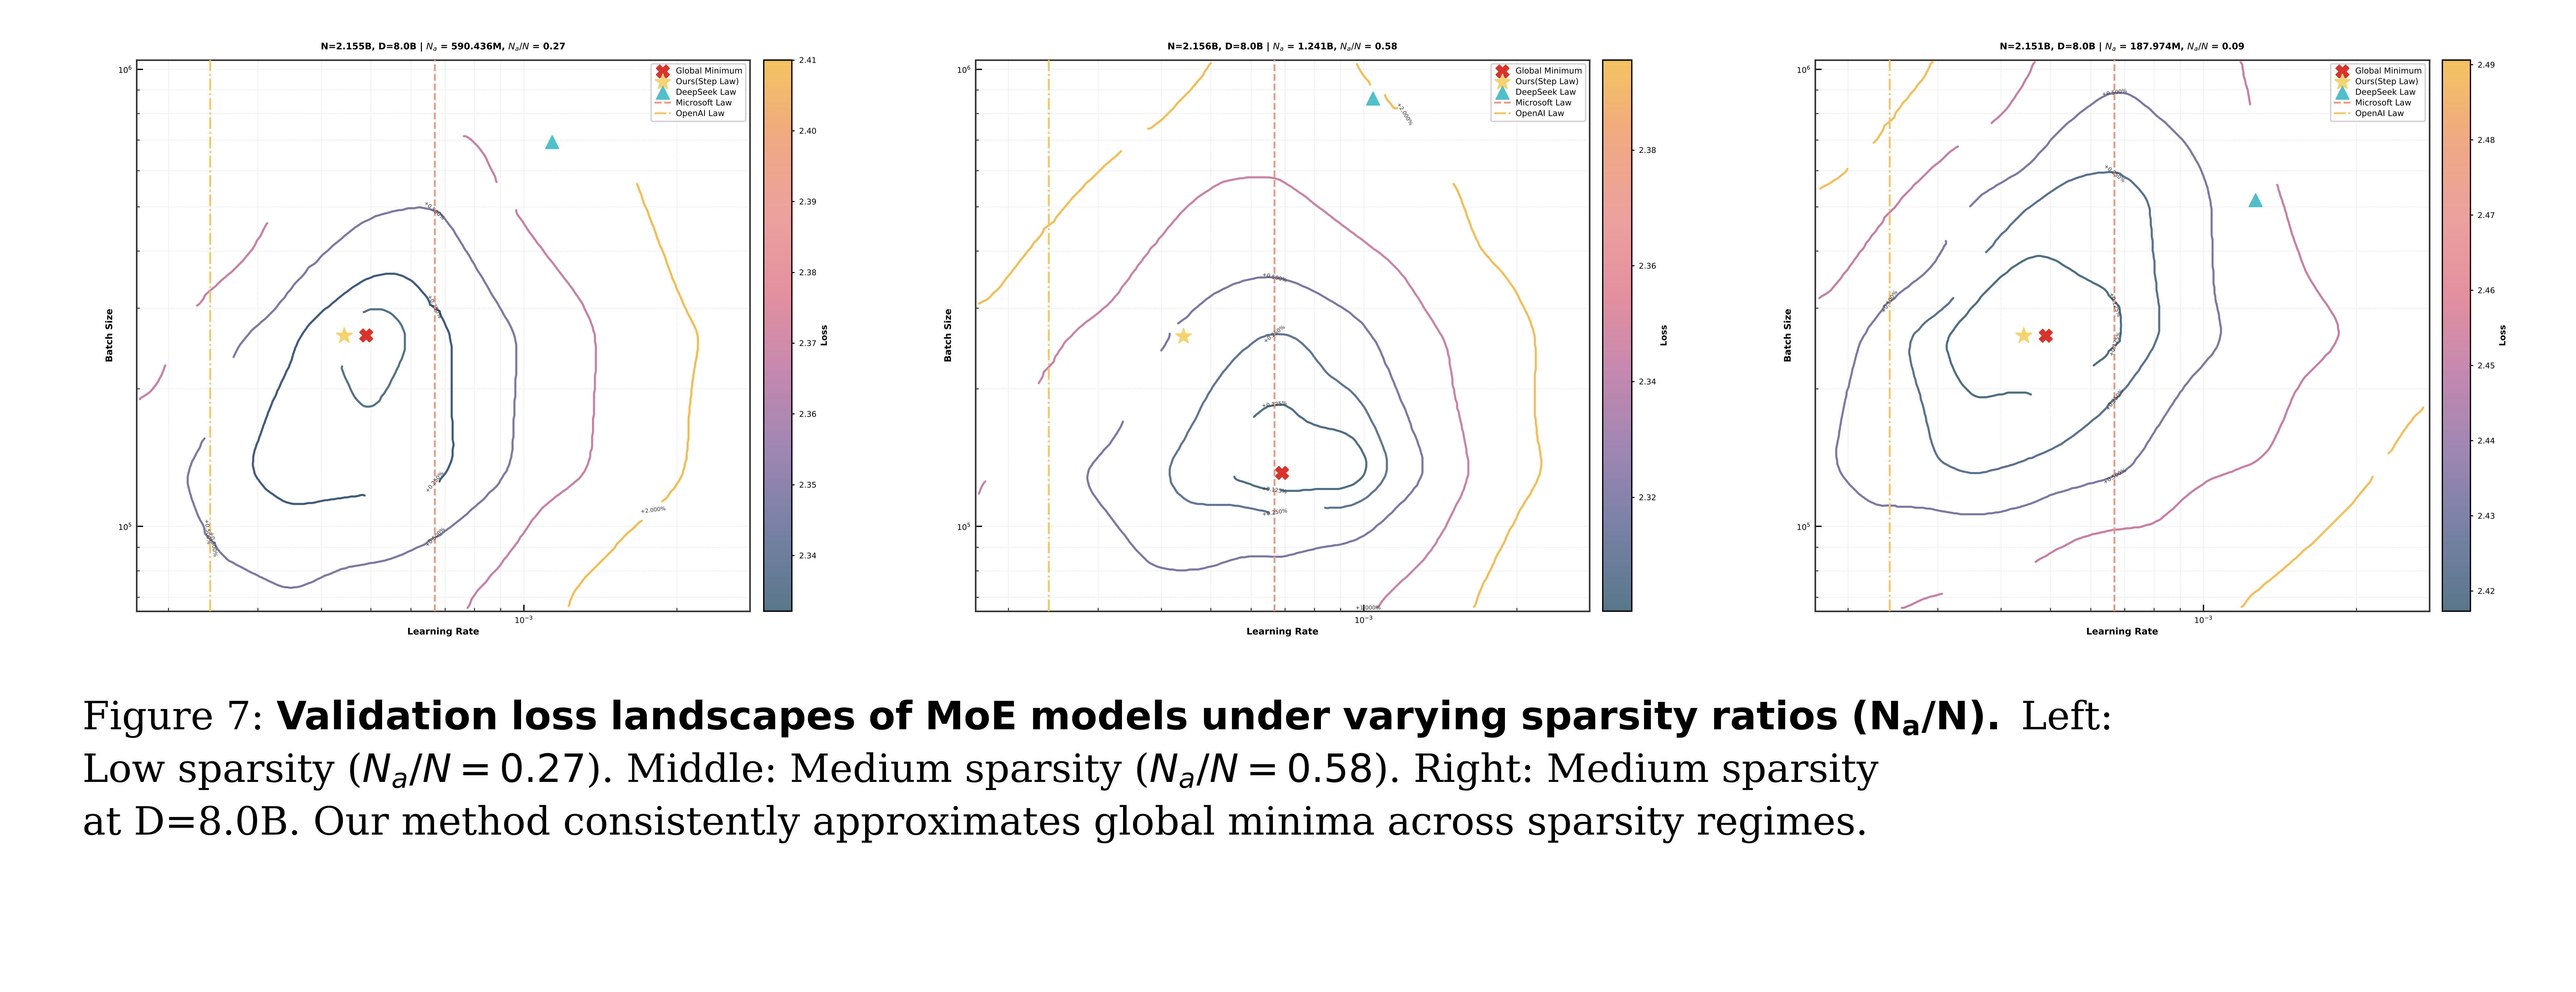
\includegraphics[width=1\linewidth]{figure7_moe_landscapes_hires.png}
\end{figure}

Generalization to other datasets!

\begin{figure}[hpbt]
    \centering
    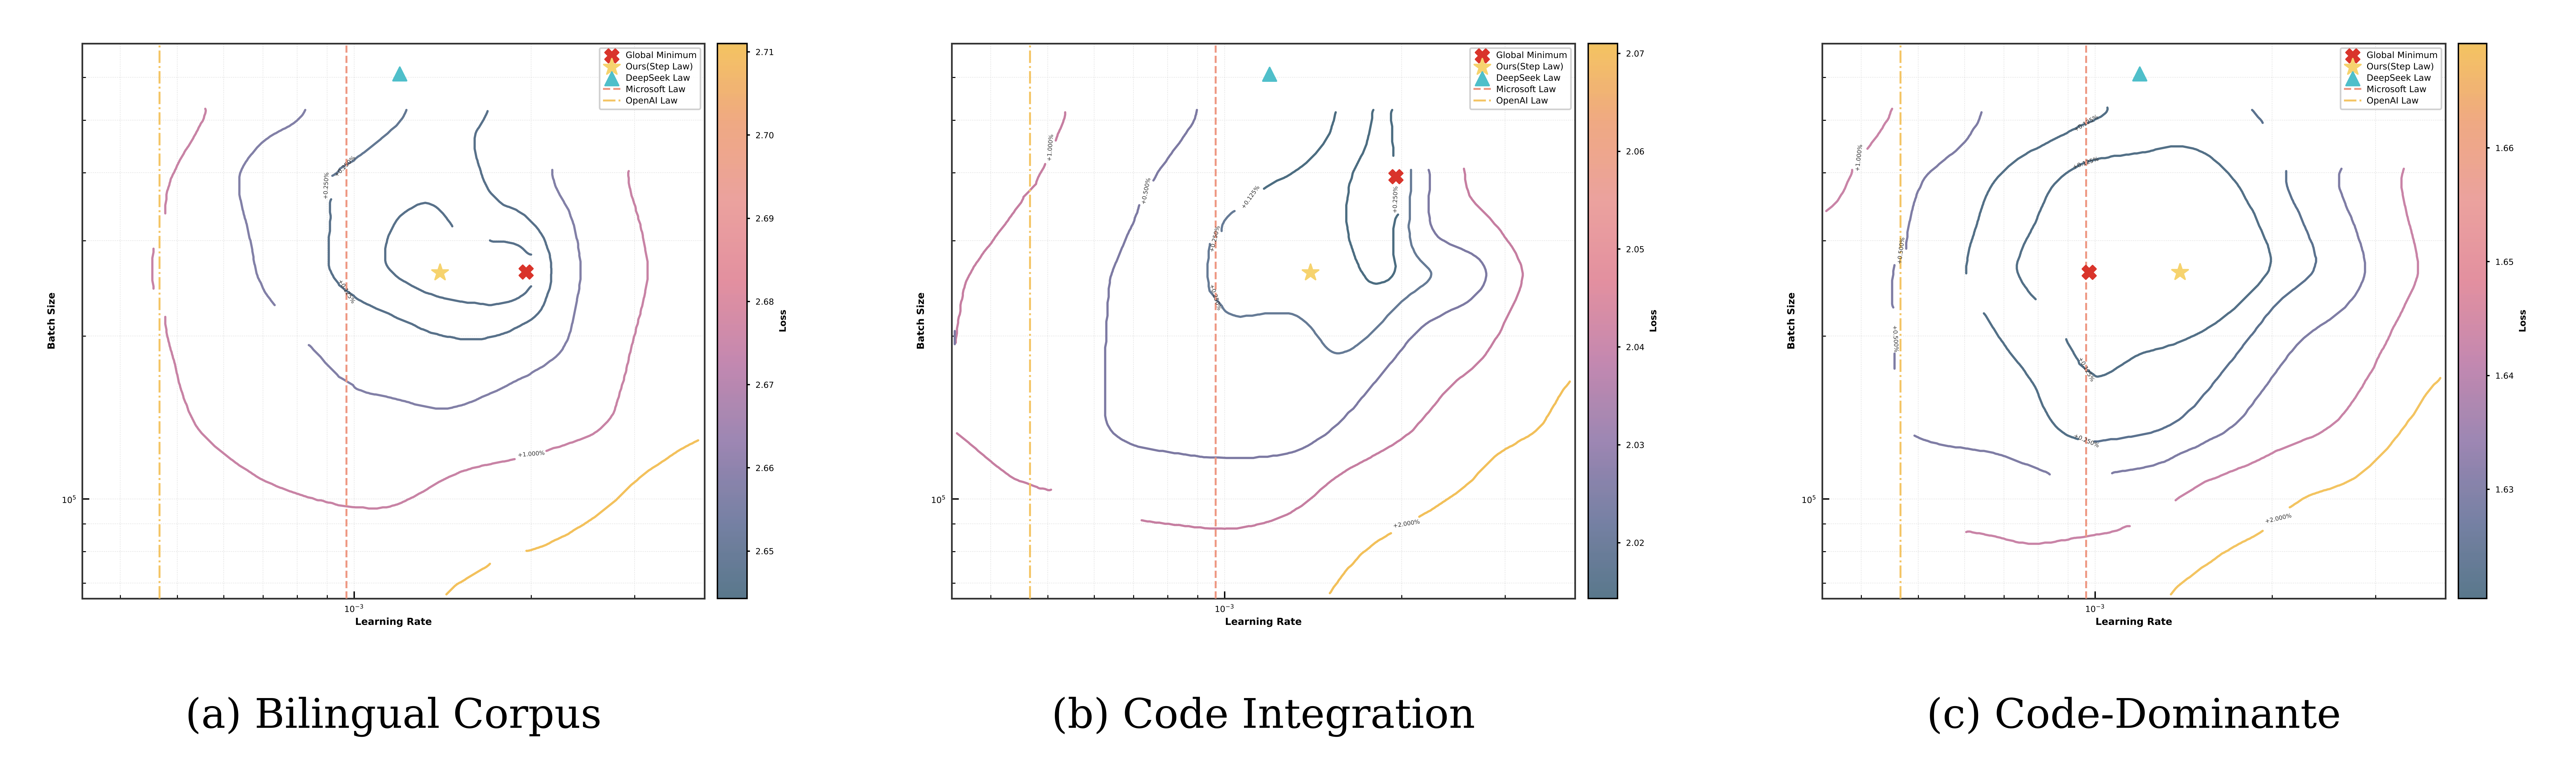
\includegraphics[width=1\linewidth]{figure_data_recipe_landscapes_hires.png}
\end{figure}

\subsection*{Optimizers and scaling}

\begin{figure}[hpbt]
    \centering
    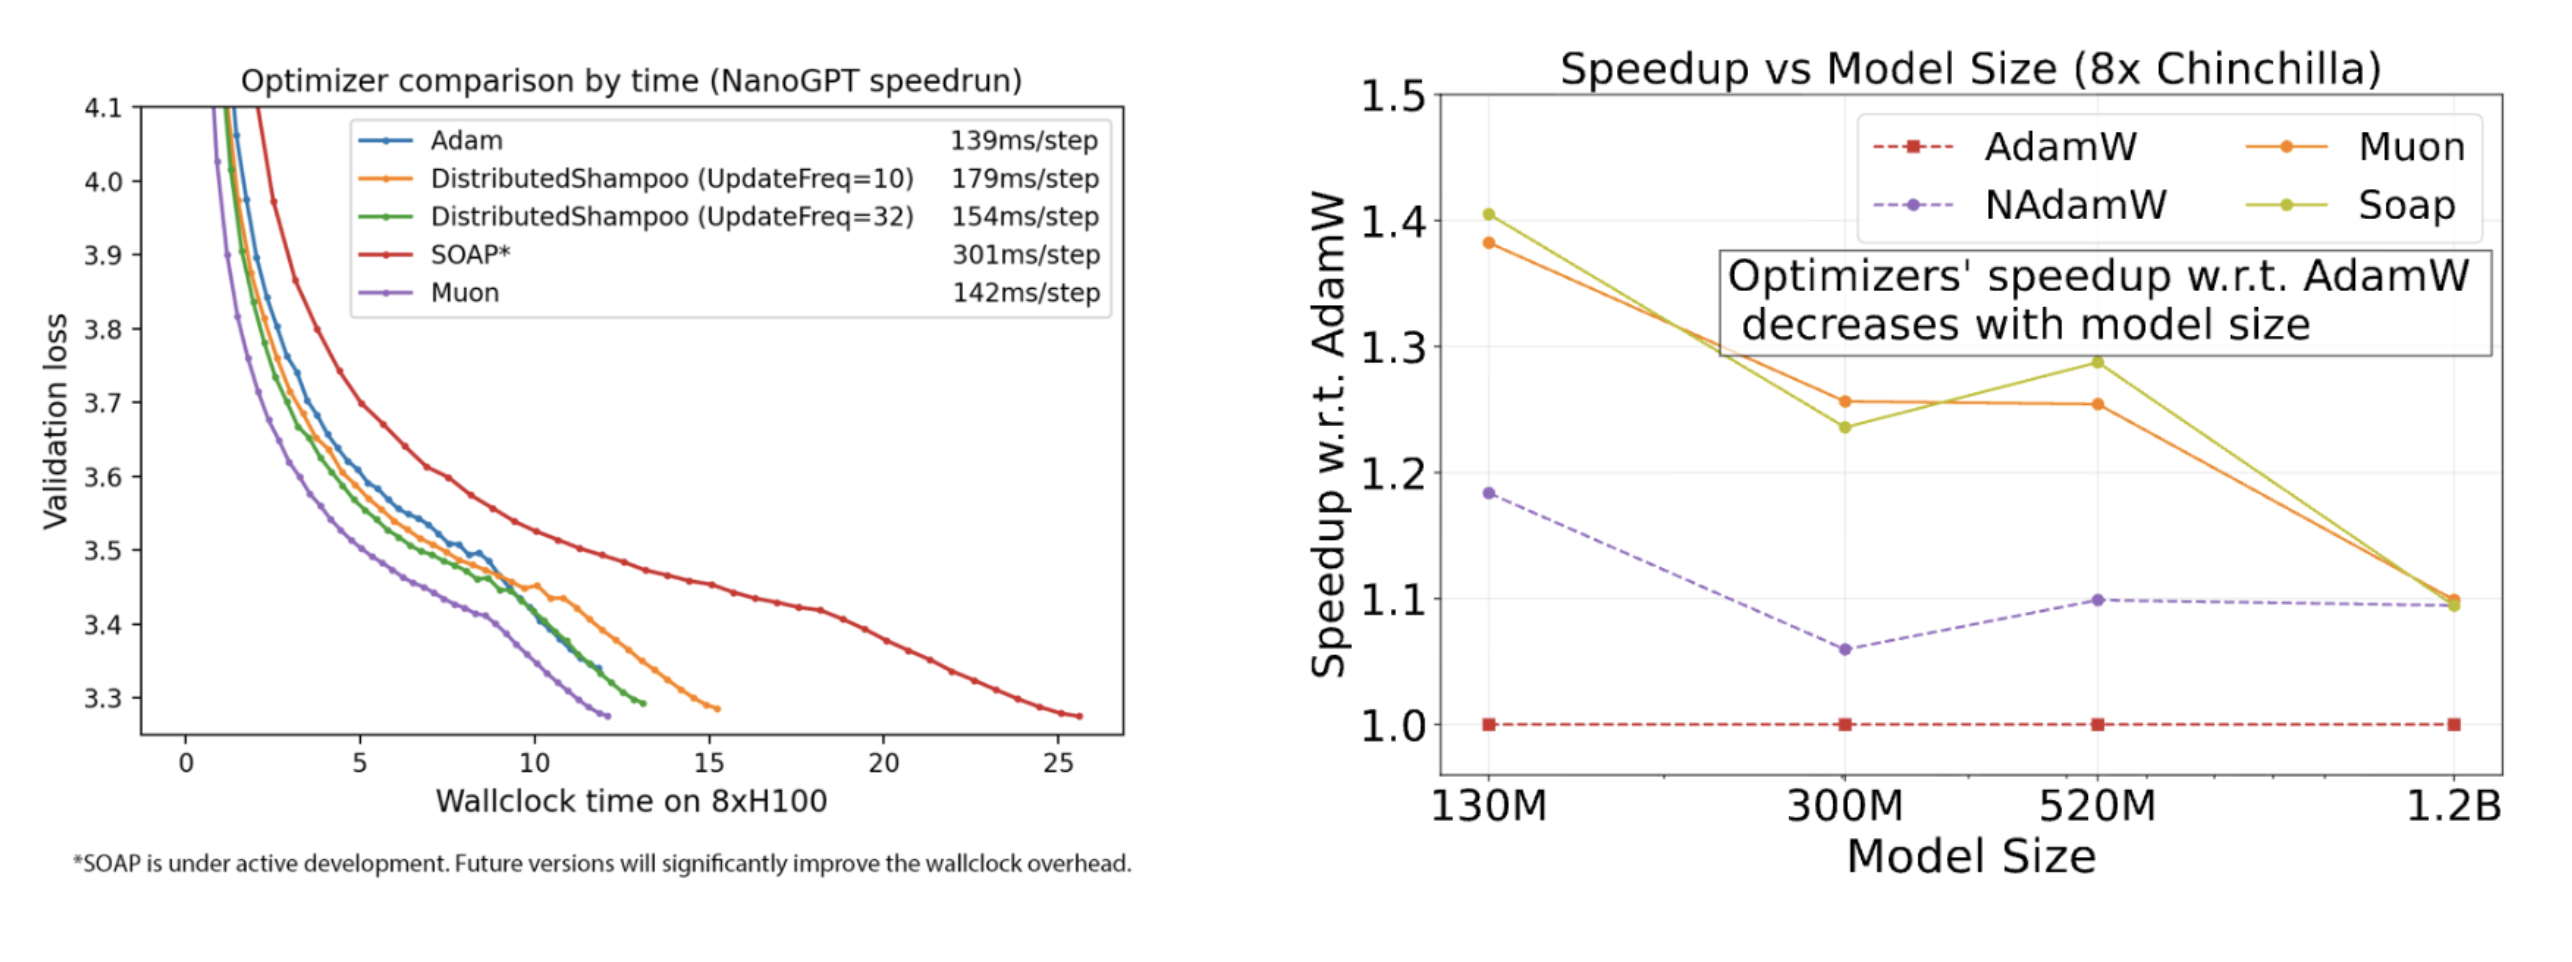
\includegraphics[width=0.83\linewidth]{optimizer.png}
\end{figure}

\begin{center}
    \textbf{Optimization is a core part of LLMs (but also tricky, due to scale dependence!)}
\end{center}

\subsection*{Problem 1 - hyper tuning is often off\ldots}

\begin{center}
    Different optimizers can require different hyperparameters!
\end{center}

\begin{figure}[hpbt]
    \centering
    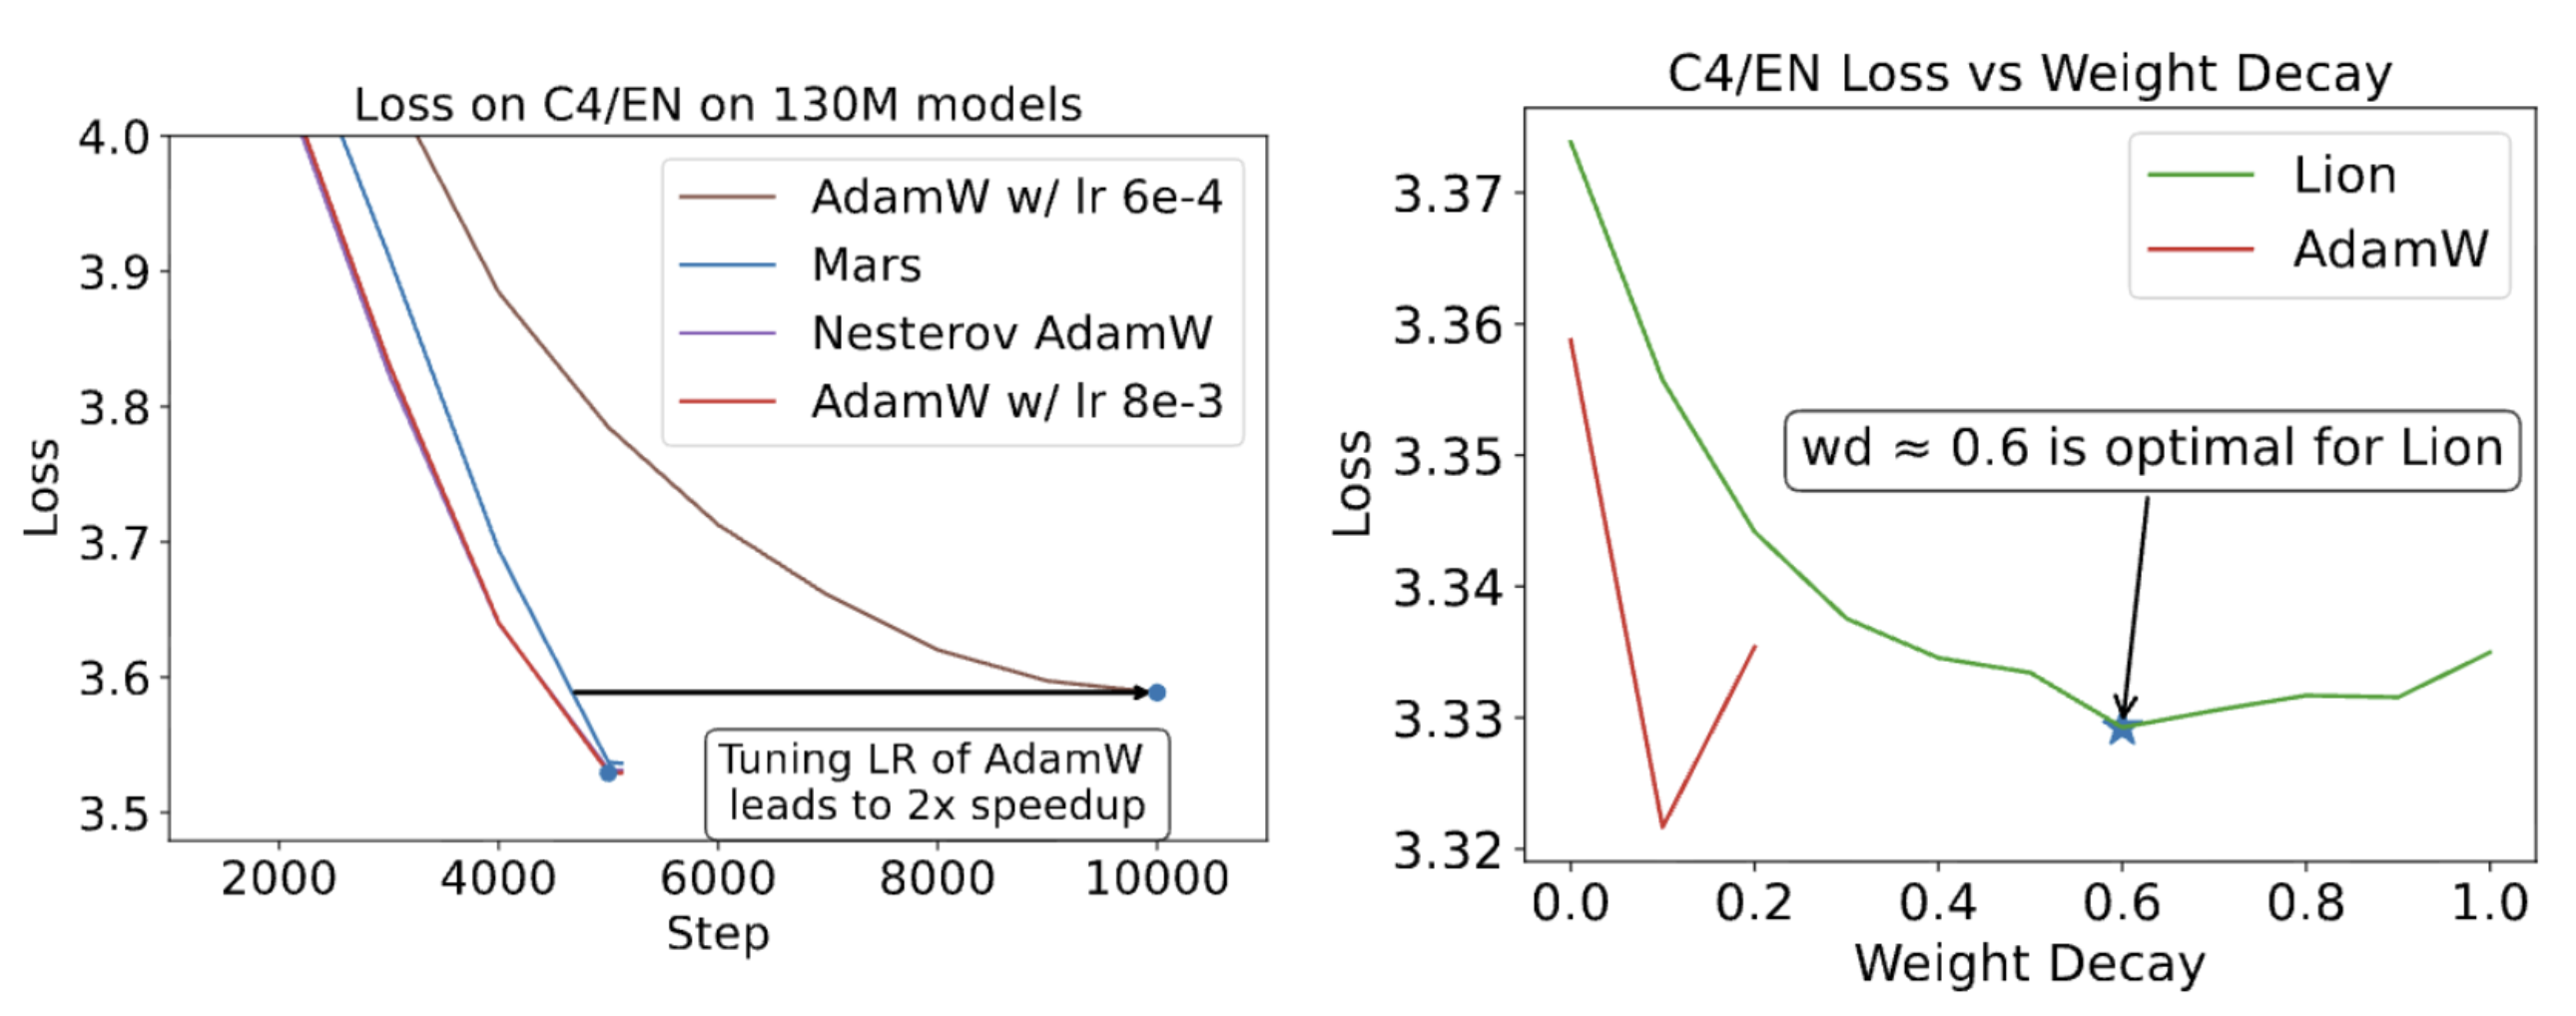
\includegraphics[width=0.75\linewidth]{pro1.png}
\end{figure}

\begin{center}
    (and likely have different optimal hyperparameter scaling)
\end{center}

\subsubsection*{Problem 2 - fairly significant scale dependence}

\begin{figure}[hpbt]
    \centering
    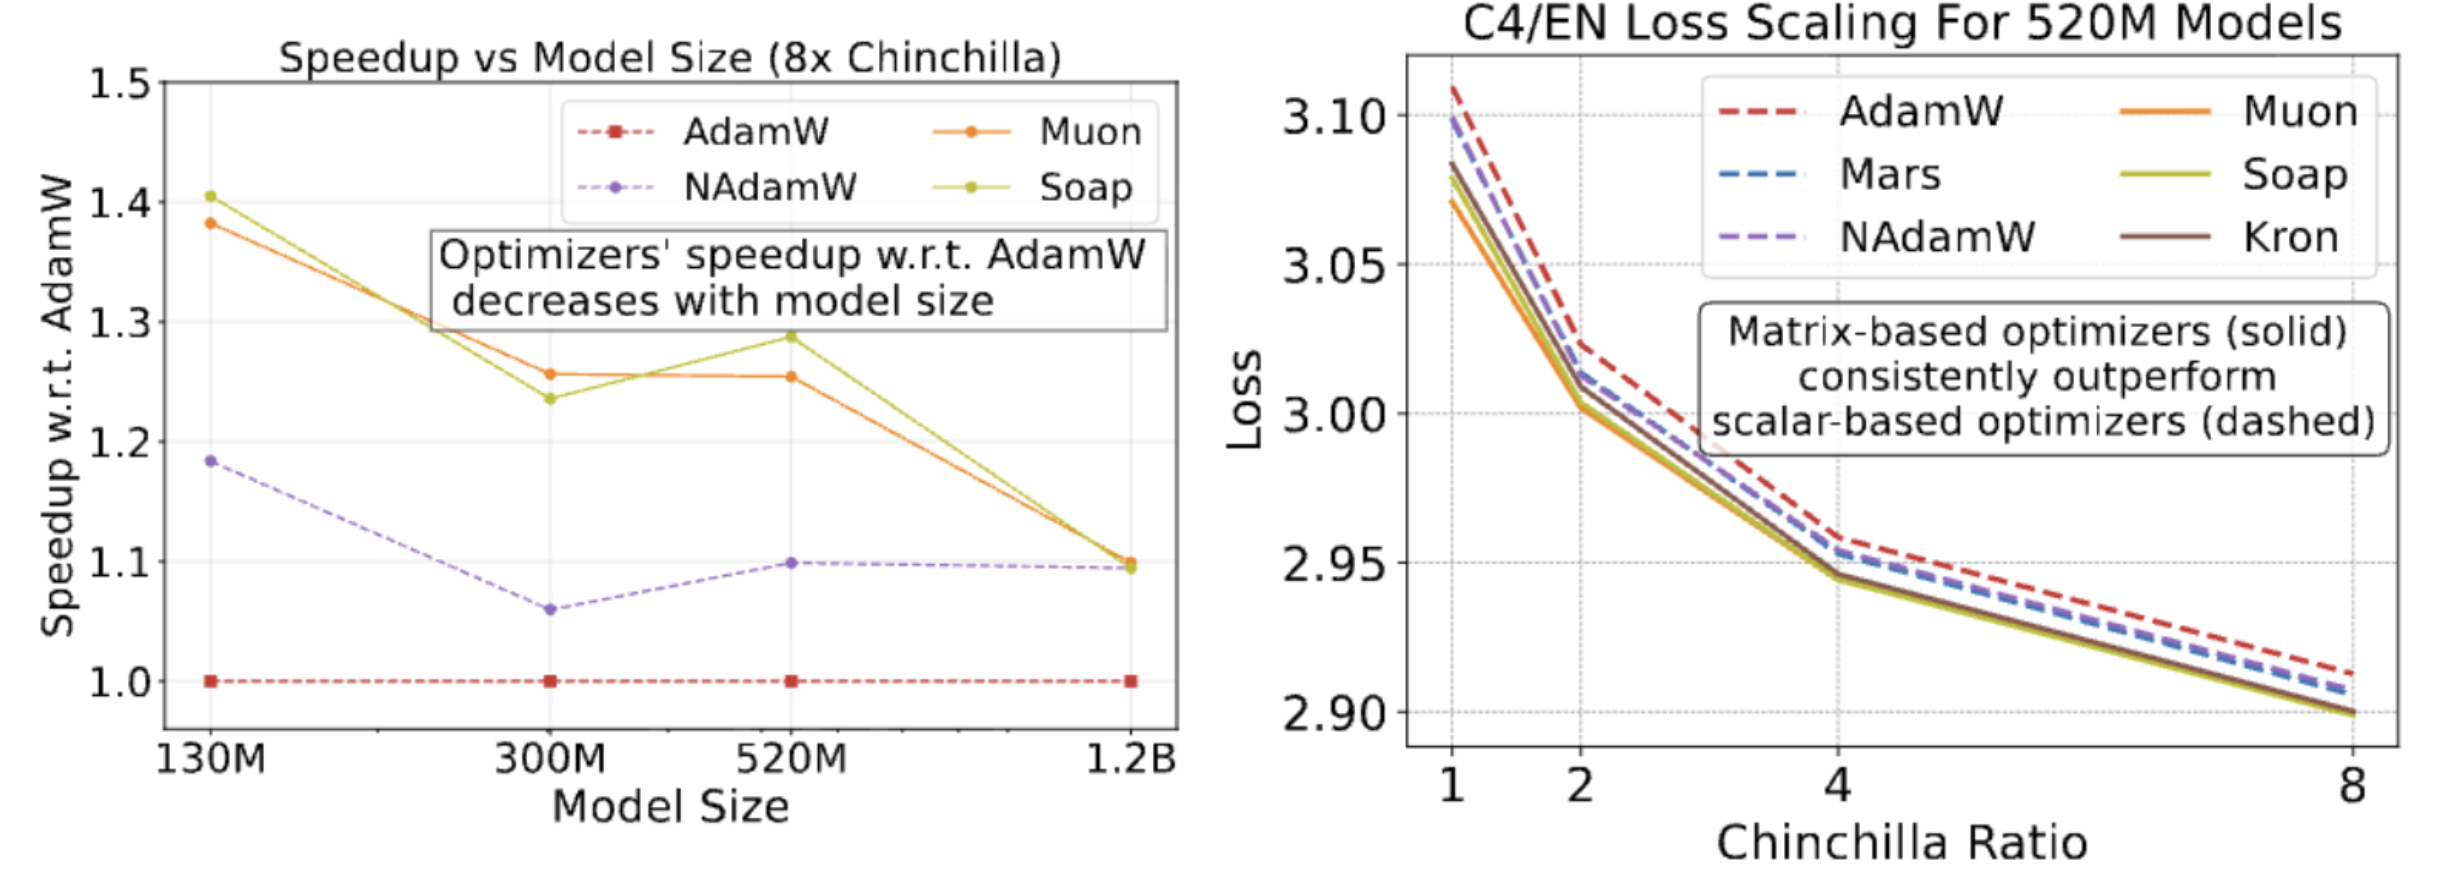
\includegraphics[width=1\linewidth]{pro2.png}
\end{figure}

\begin{center}
    General algorithm development note - \textit{always} check scaling with respect to compute and Chinchilla ratios. These are often major confounders to performance!
\end{center}

\subsubsection*{Problem 2.5 - establishing scaling is nontrivial!}

Sometimes, a good looking scaling can blow up!

\begin{figure}[hpbt]
    \centering
    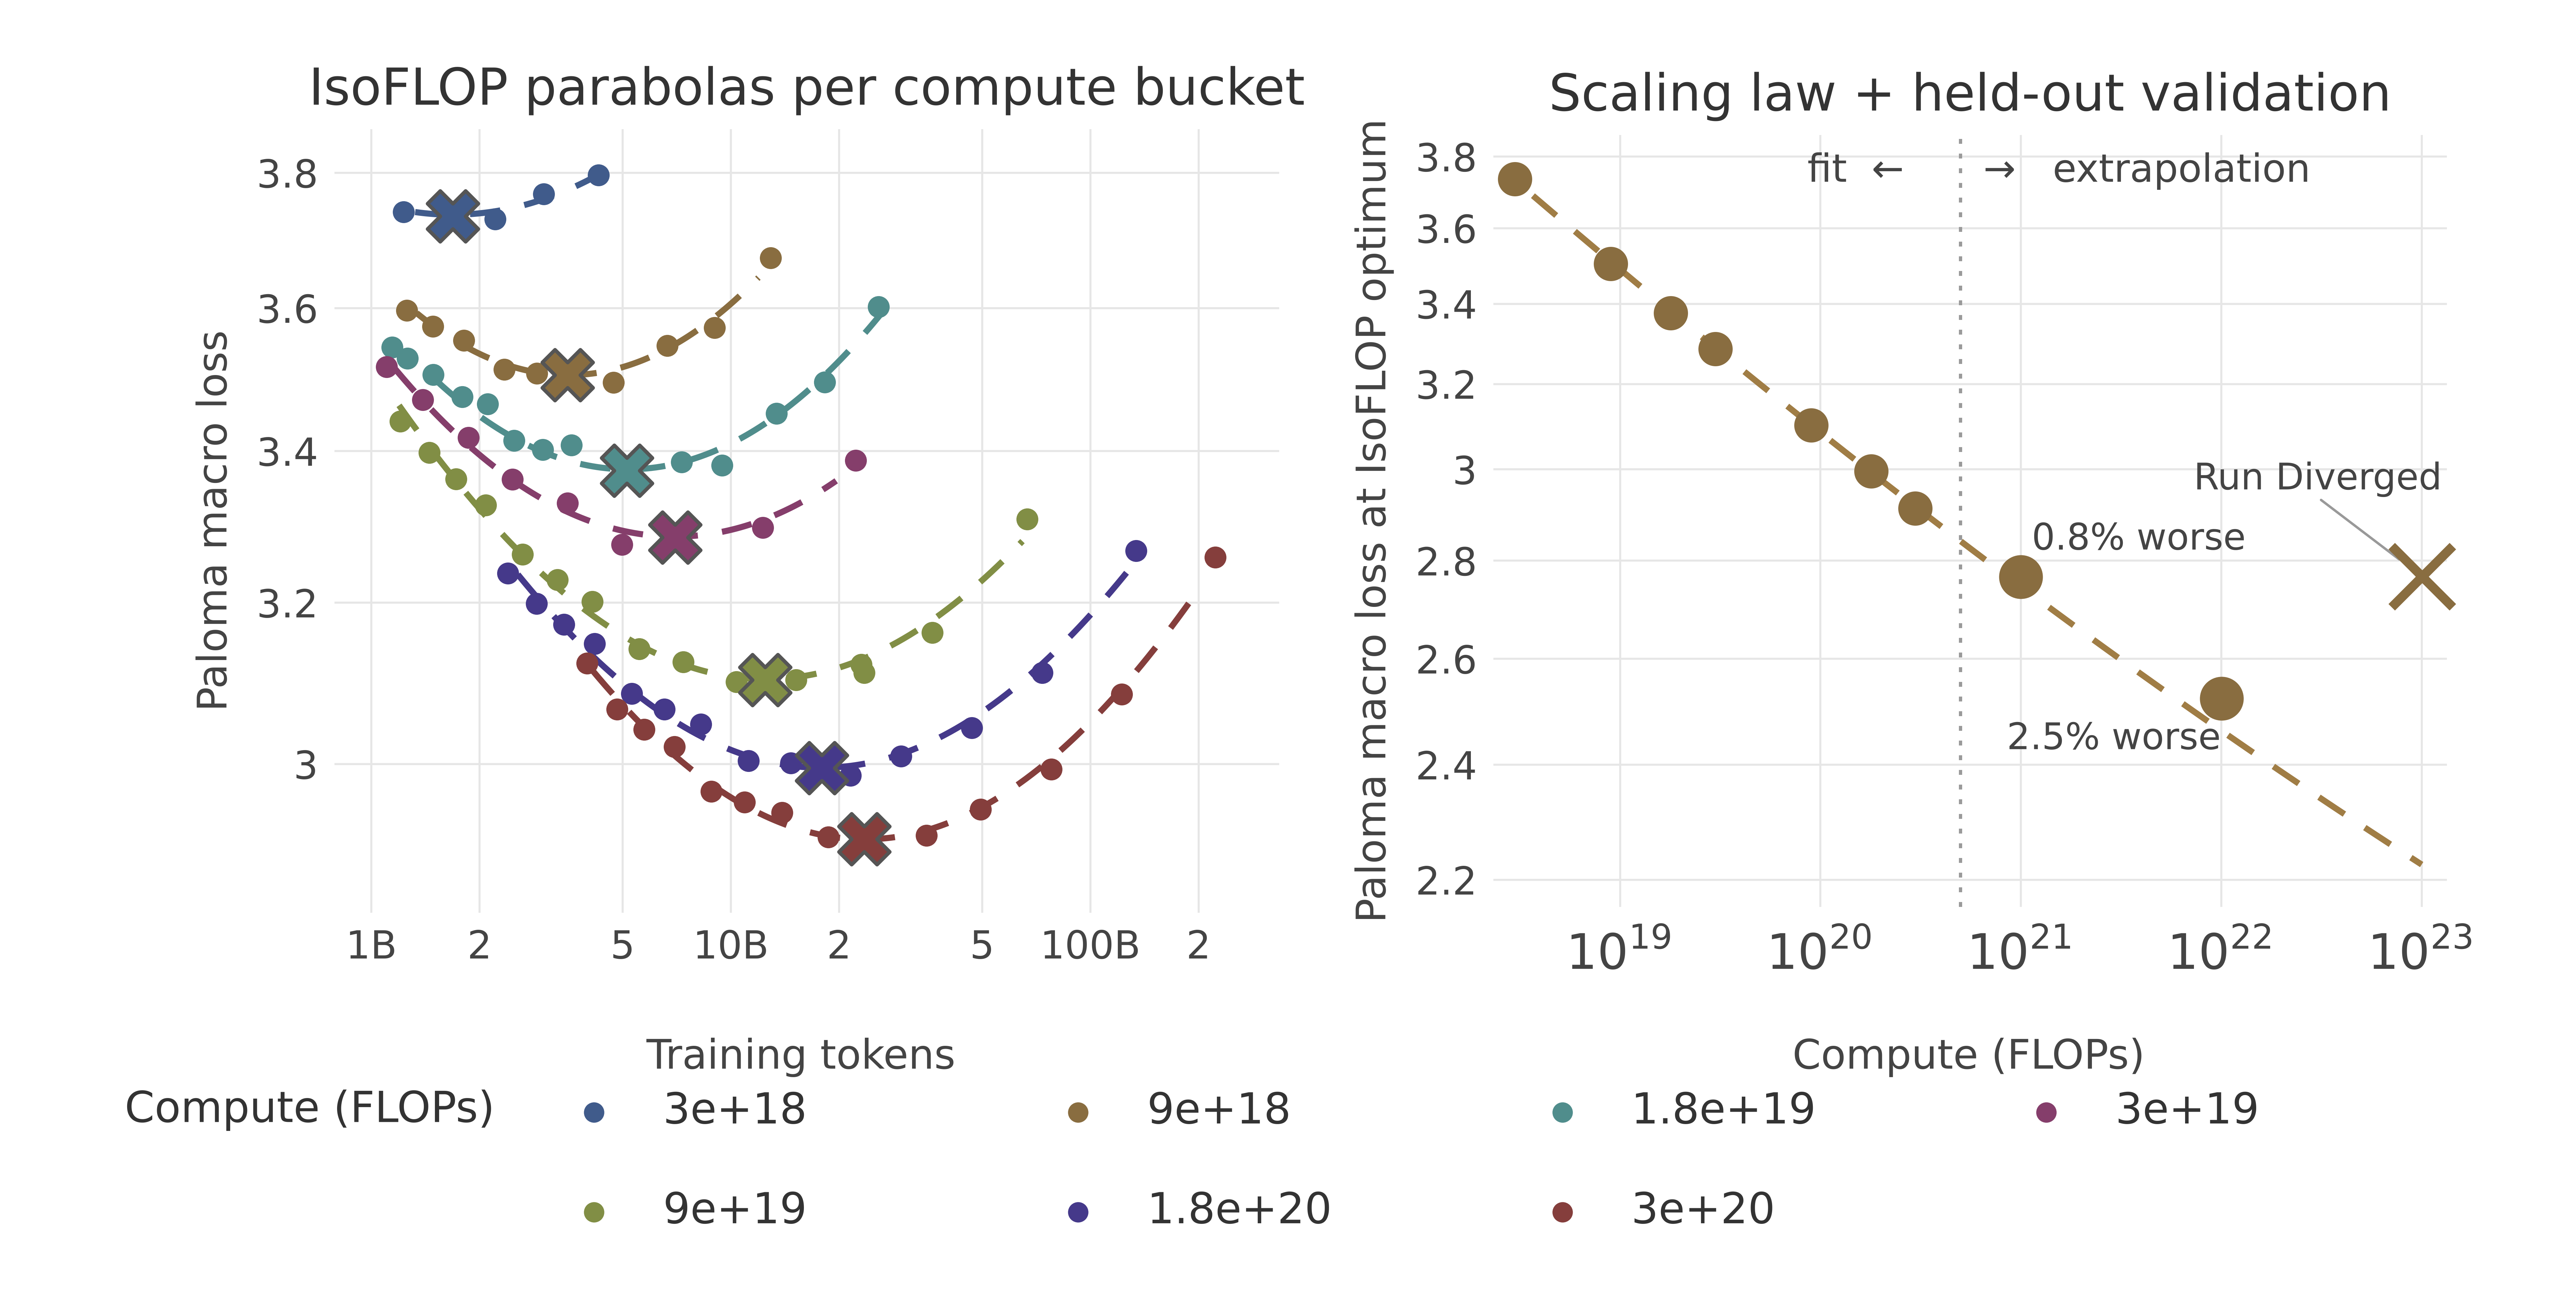
\includegraphics[width=1\linewidth]{figure_isoflop_scaling_hires.png}
\end{figure}

\subsection*{Muon and scaling}

\begin{center}
    Optimizer for ``matrix-valued'' parameters.
\end{center}

\begin{figure}[H]
    \centering
    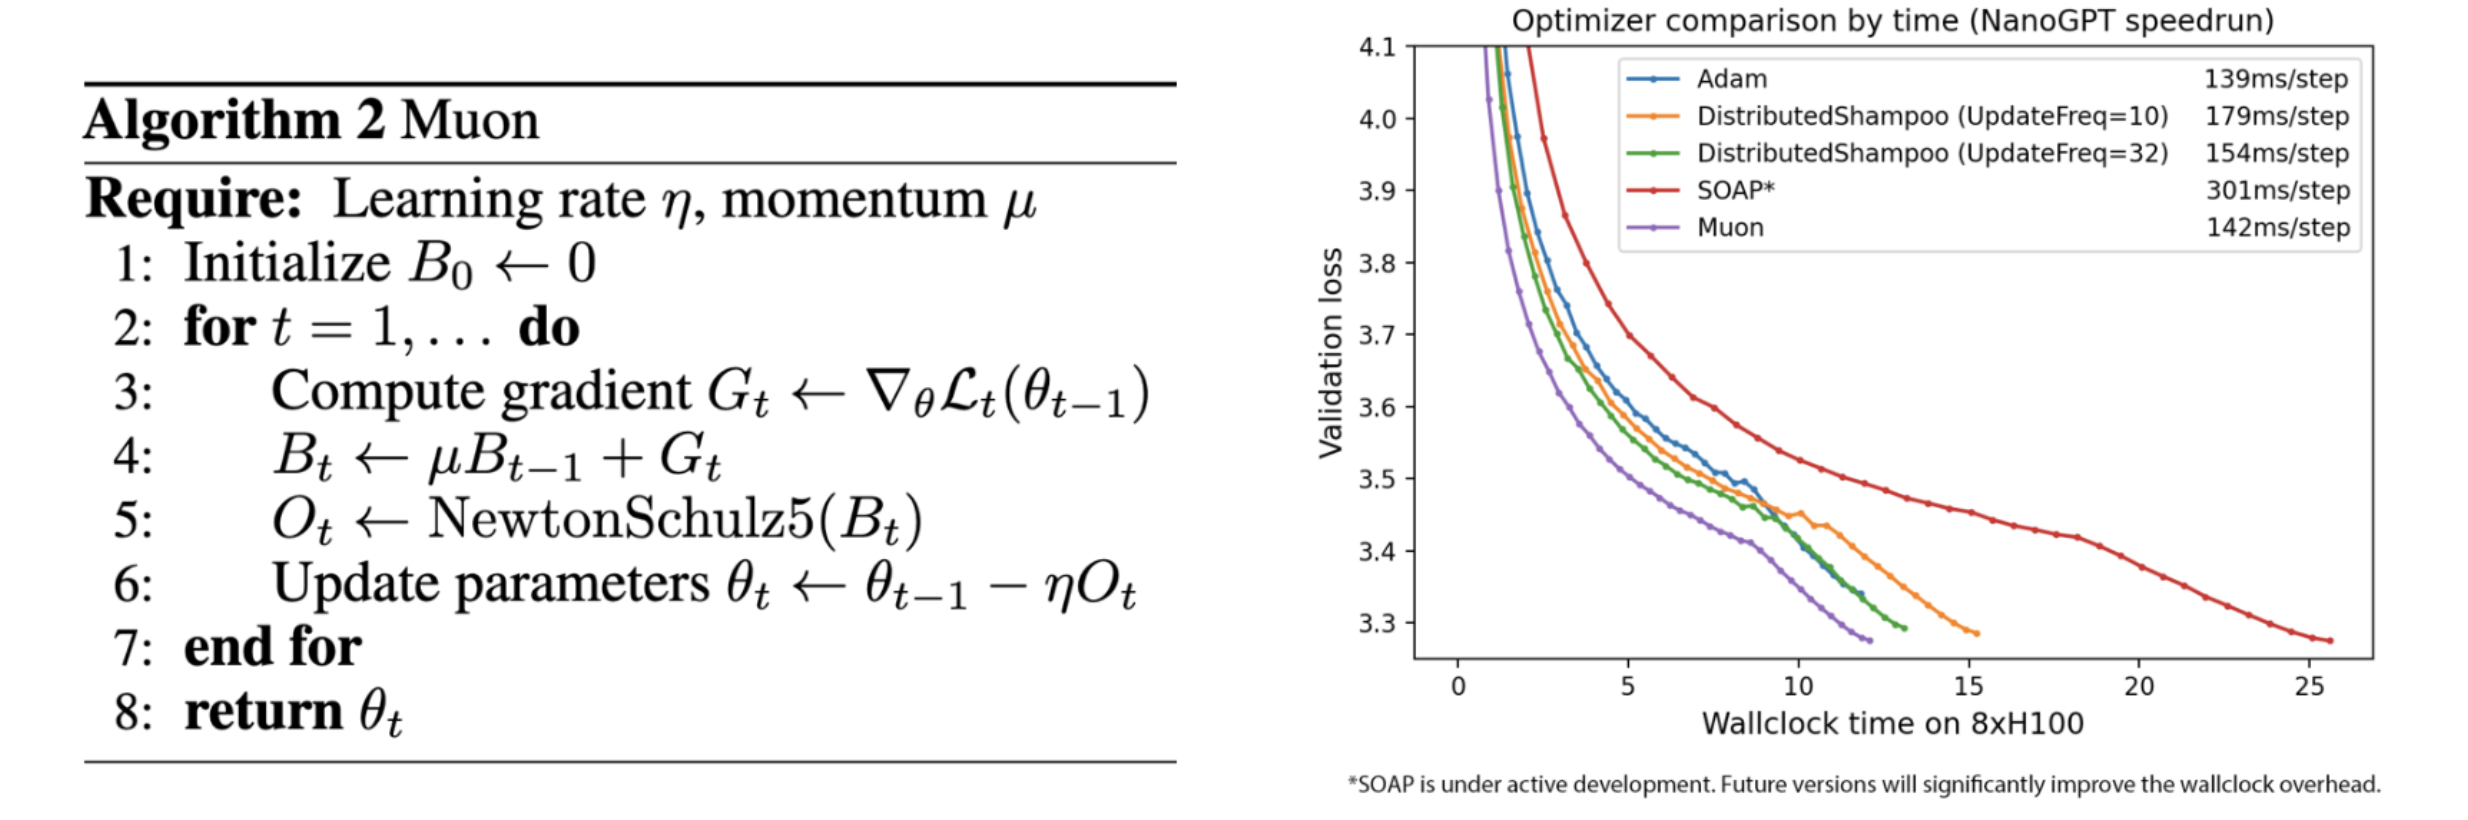
\includegraphics[width=1\linewidth]{muon.png}
\end{figure}

\begin{center}
    Newton--Schulz (approximately) orthogonalizes the matrix \(B_t = USV^T \to UV^T\).
\end{center}

\begin{figure}[hpbt]
    \centering
    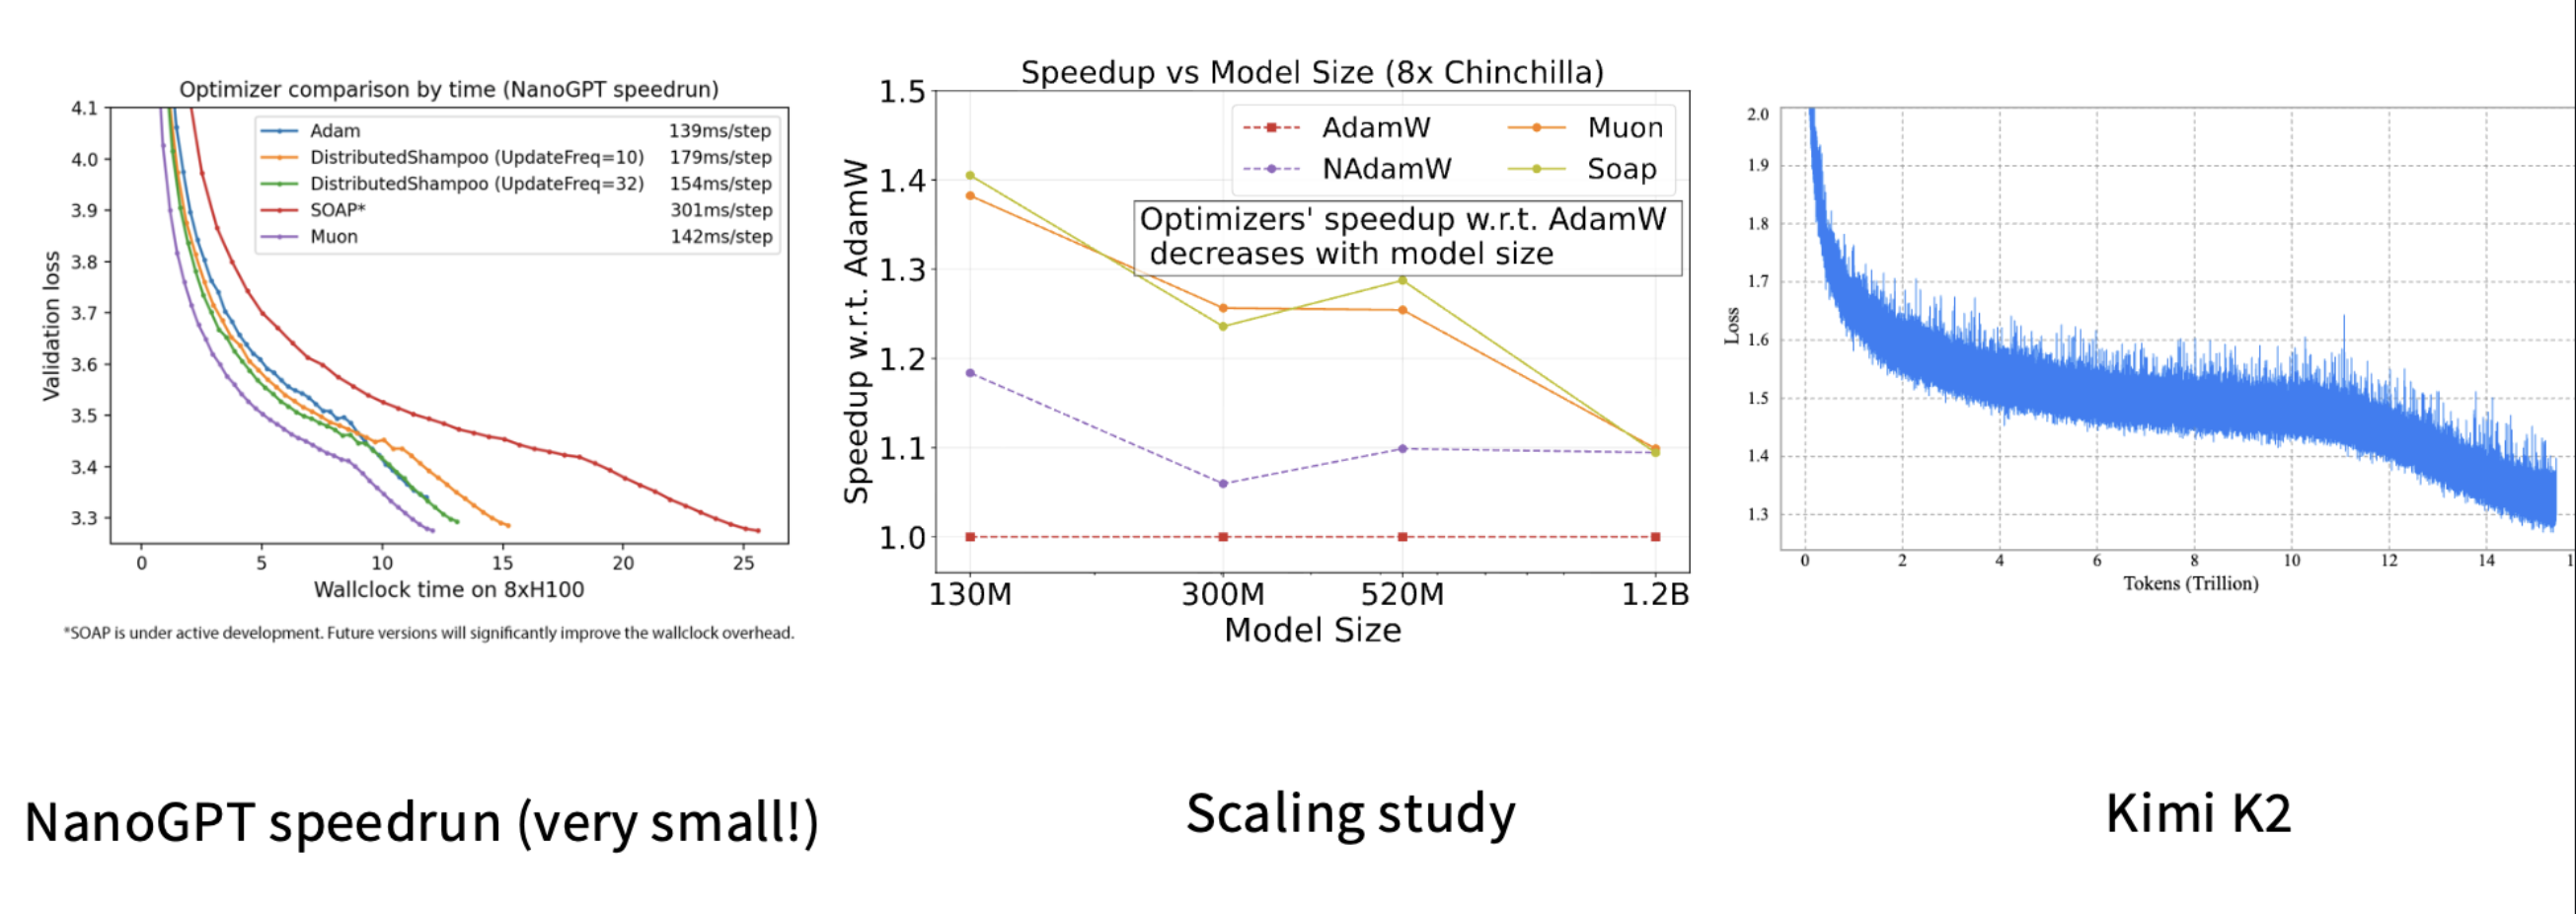
\includegraphics[width=1\linewidth]{muon_scale.png}
\end{figure}

\begin{center}
    Scaling gains are tricky to measure, but clearly muon ``works'' at scale.
\end{center}

\subsubsection*{Maximal update parameterization - in depth}

Recall - the maximal update parameterization makes appealing claims.

\begin{center}
    Scale-invariant hyperparameter tuning would be very nice.
\end{center}

How does it work, and does it work in practice?

\begin{itemize}
    \item CerebrasGPT - 0.1 to 13B models trained with the Chinchilla recipe.
    \item \textbf{Core finding} - using muP parameterization makes scaling more stable
\end{itemize}

\subsection*{What is muP?}

\begin{figure}[hpbt]
    \centering
    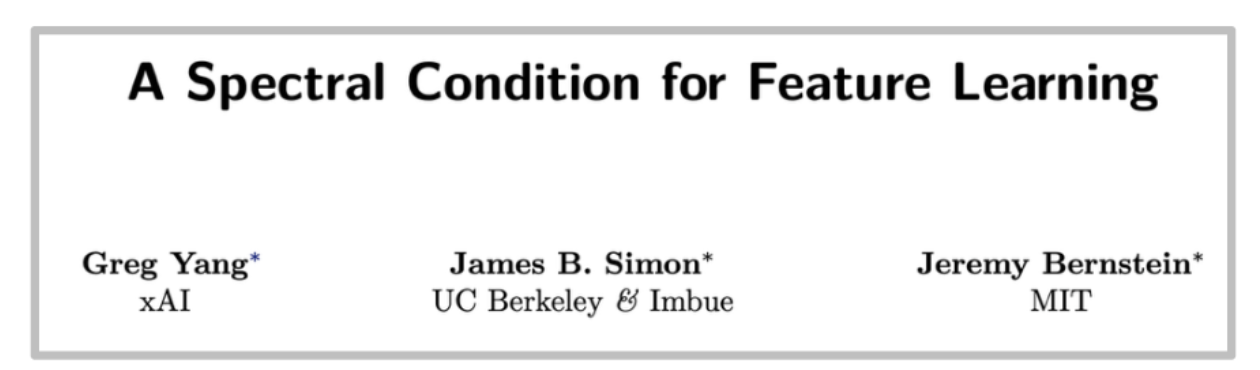
\includegraphics[width=1\linewidth]{muP.png}
\end{figure}

\textbf{muP} is based off the following assertion. As a function of the width of the network \(n_l\) \ldots

\begin{itemize}
    \item \textbf{A1}: The activations at initialization should remain \(\Theta(1)\)
    \item \textbf{A2}: After one gradient step, the change in activation should be \(\Theta(1)\)
\end{itemize}

\begin{center}
    Note: if individual activations are \(\Theta(1)\), then the norm should be \(\Theta(\sqrt{n_l})\).
\end{center}

\subsubsection*{Deriving muP (A1)}

Suppose that we have a simple, deep linear network (\(h_l = W_l h_{l-1}\)) and we initialize \(W_l \sim N(0,\sigma^2 I_{n_l \times n_{l-1}})\); then by basic matrix concentration \(\Vert W_l \Vert_{*} \to \sigma(\sqrt{n_{l-1}} + \sqrt{n_l})\) and
\[
    \Vert h_l \Vert_2 \approx \Vert W_l \Vert_{*} \Vert h_{l-1} \Vert_2.
\]

Now let's pick
\[
    \sigma = \frac{\sqrt{n_l}}{\sqrt{n_{l-1}}}(\sqrt{n_l} + \sqrt{n_{l-1}})^{-1} = \Theta\left(\frac{1}{\sqrt{n_{l-1}}}\min\left(1,\sqrt{\frac{n_l}{n_{l-1}}}\right)\right).
\]

What happens?
\begin{itemize}
    \item \textbf{Inductive assumption} - \(\Vert h_{l-1} \Vert_2 = \Theta(\sqrt{n_{l-1}})\)
    \item \textbf{Matrix concentration} - \(\Vert W_l \Vert_{*} \to \sigma(\sqrt{n_l} + \sqrt{n_{l-1}}) = \frac{\sqrt{n_l}}{\sqrt{n_{l-1}}}\)
\end{itemize}
\begin{equation*}
    \boxed{\Vert h_l \Vert_2 = \sqrt{n_l} + o(\sqrt{n_l})}
\end{equation*}

[Comments - this is a kind of ``worst-case'' derivation - the \(\approx\) is an upper bound]

\subsubsection*{Deriving muP (A2)}

Now we need to deal with updates. Suppose we have the update \(\Delta W_l\) on the weights. For SGD, on a linear layer, this looks like a rank-one loss-activation outer product:
\[
    \Delta W_l = -\eta_{l}\nabla_{h_l} \ell \, h_{l-1}^T.
\]

Thus, \(\Vert \Delta W_l h_{l-1} \Vert_2 = \Vert \Delta W_l \Vert_{*} \Vert h_{l-1} \Vert_2\). Note that we have the update
\[
    \Delta h_l = W_l \Delta h_{l-1} + \Delta W_l(h_{l-1} + \Delta h_{l-1}).
\]

Assuming that the leading order terms don't cancel, we see that
\begin{itemize}
    \item \(W_l \Delta h_{l-1} = \Theta(\sqrt{n_l})\) from induction assumption \(+\) condition A1 argument.
    \item \(\Delta W_l h_{l-1} = \Vert \Delta W_l \Vert_{*} \sqrt{n_{l-1}}\) from above, thus \(\Vert \Delta W_l \Vert_{*} = \Theta\left(\frac{\sqrt{n_l}}{\sqrt{n_{l-1}}}\right)\).
    \item \(\Delta W_l \Delta h_{l-1} = O(\Vert \Delta W_l \Vert_{*} \sqrt{n_{l-1}})\).
\end{itemize}

\begin{center}
    Recall - the key is to pick LR such that \(\Vert \Delta W_l \Vert_{*} \sqrt{n_{l-1}} = \Theta(\sqrt{n_l})\). How can we do that?
\end{center}

Suppose that the loss update \textit{also} scales \(\Theta(1)\). Then we can write down
\[
    \Delta \ell \approx \Theta(\langle\Delta W_l, \nabla_{W_l}\ell\rangle) = \Theta(\Vert \Delta W_l \Vert_F \Vert \nabla_{W_l}\ell \Vert_F) = \Theta(\Vert \Delta W_l \Vert_{*} \Vert \nabla_{W_l} \ell \Vert_{*})
\]
where we use that \(\Delta W_l = -\eta_l \nabla_{W_l} \ell\) in standard SGD updates (and that both are rank one, so Frobenius and operator norms coincide). Now plug in \(\Delta \ell = \Theta(1)\), \(\Vert \Delta W_l \Vert_{*} = \Theta\left(\frac{\sqrt{n_l}}{\sqrt{n_{l-1}}}\right)\) to get that \(\Vert \nabla_{W_l} \ell \Vert_{*} = \Theta\left(\frac{\sqrt{n_{l-1}}}{\sqrt{n_l}}\right)\).

\begin{center}
    Finally, from the previous page, recall that \(\Delta W_l = -\eta_l \nabla_{W_l} \ell\), so \(\eta_l = \Vert \Delta W_l \Vert_{*} / \Vert \nabla_{W_l} \ell \Vert_{*}\).
\end{center}
\begin{equation*}
    \boxed{\eta_l = \Theta\left(\frac{n_l}{n_{l-1}}\right)}
\end{equation*}

So, what is (baby) muP about? Controlling activations (and changes) via \(W\) and \(\Delta W\)
\begin{itemize}
    \item \textbf{Initialization (stdev)}: Set to \(\Theta\left(\frac{1}{\sqrt{n_{l-1}}}\min\left(1,\sqrt{\frac{n_l}{n_{l-1}}}\right)\right)\)
    \item \textbf{Learning rates}: Set to \(\Theta\left(\frac{n_l}{n_{l-1}}\right)\)
\end{itemize}

Compared to ``standard'' parameterizations - these set
\begin{itemize}
    \item \textbf{Initialization}: Set to \(\frac{1}{\sqrt{n_{l-1}}}\)
    \item \textbf{Learning rates}: Set to \(\Theta(1)\)
\end{itemize}

\textbf{Differences} - LR changes for Adam, also init diffs when fan-in \(>\) fan-out.

\subsubsection*{Deeper dive into muP}

Recall - muP is a scaling procedure for hyperparams (as a function of width).

\begin{figure}[H]
    \centering
    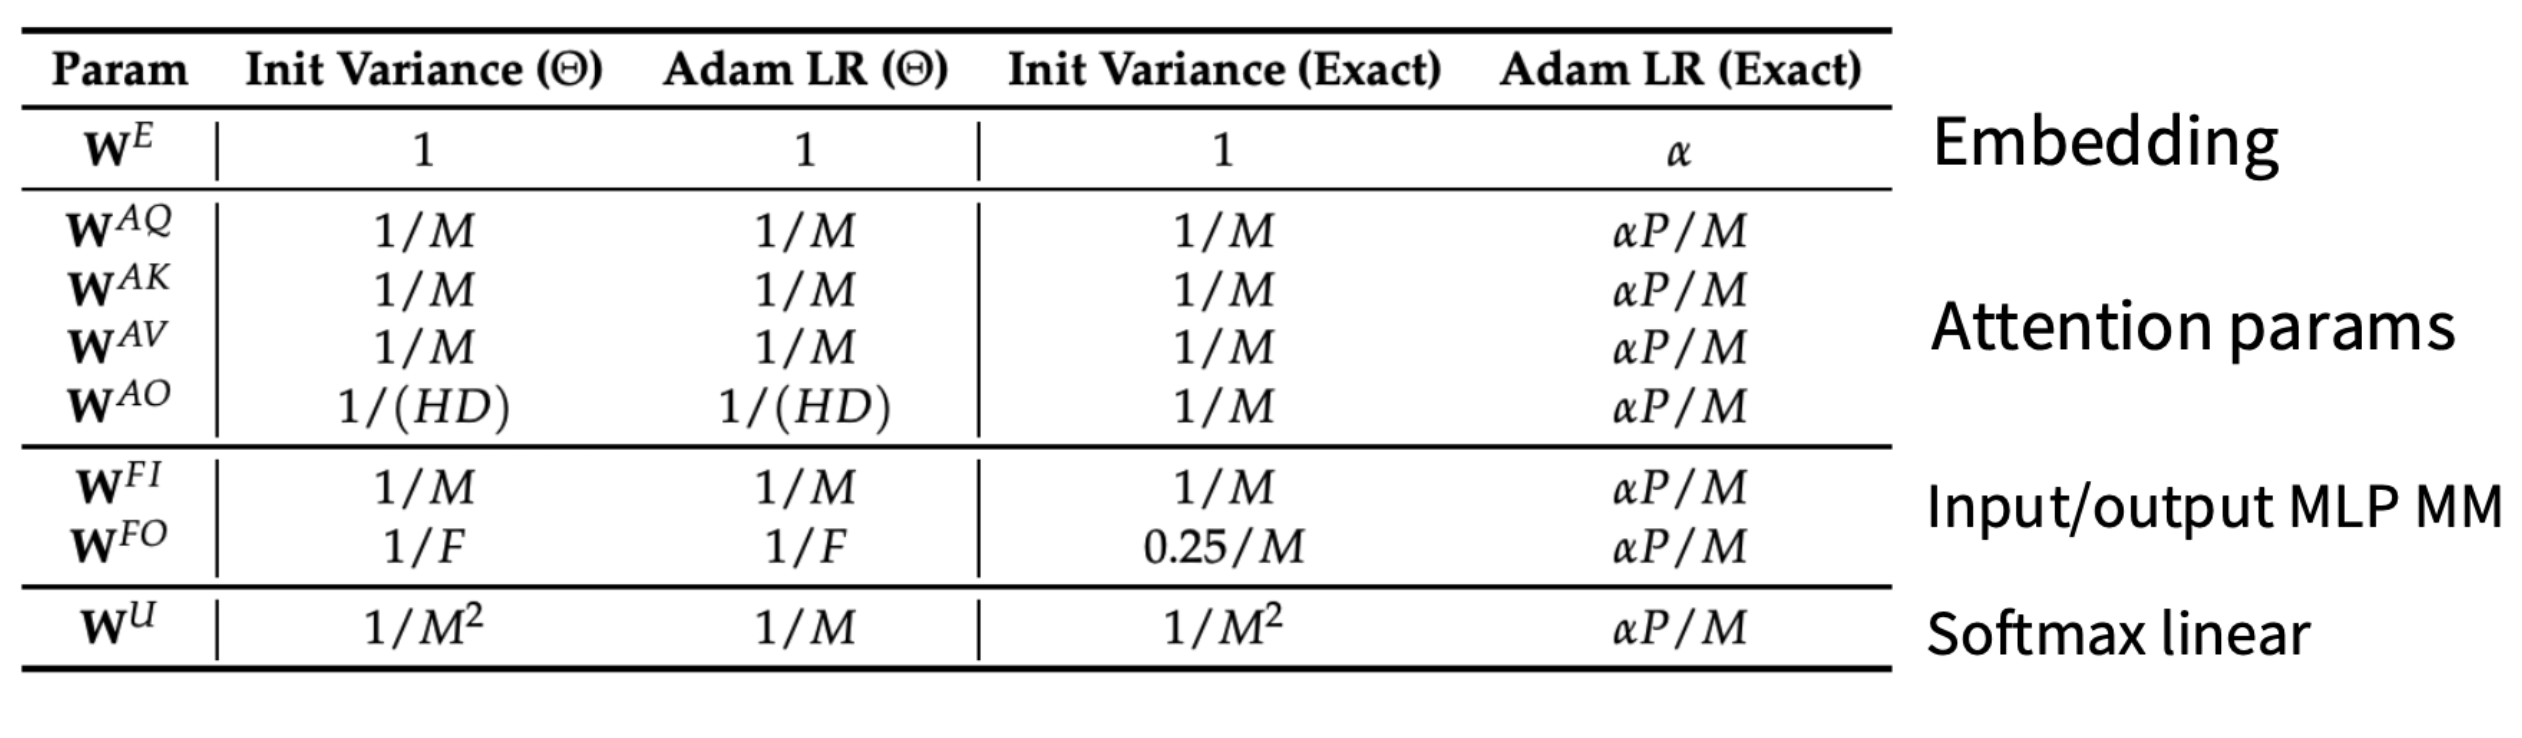
\includegraphics[width=1\linewidth]{chart.png}
\end{figure}

\begin{center}
    In addition, \(\mu\)P uses an attention scale of \(\tau^{-1} = \Theta(1/D)\) instead of the usual \(\tau^{-1} = 1 / \sqrt{D}\). For simplicity, we use \(\tau^{-1} = 1 / D\), since in preliminary experiments we observed only a small improvement from using smaller multiples of \(1 / D\). Note that for \(D\) fixed across model widths \(M\), any constant \(\tau^{-1} \neq 0\) technically complies with \(\mu\)P [Yang et al. (2021)] but in experiments, \(\tau^{-1}\) will be shown to have a major impact on performance and transfer.
\end{center}

\subsubsection*{Replicating muP}

\textbf{Q1}: Does muP work as claimed? When we scale widths, is optimal LR constant?

\begin{figure}[hpbt]
    \centering
    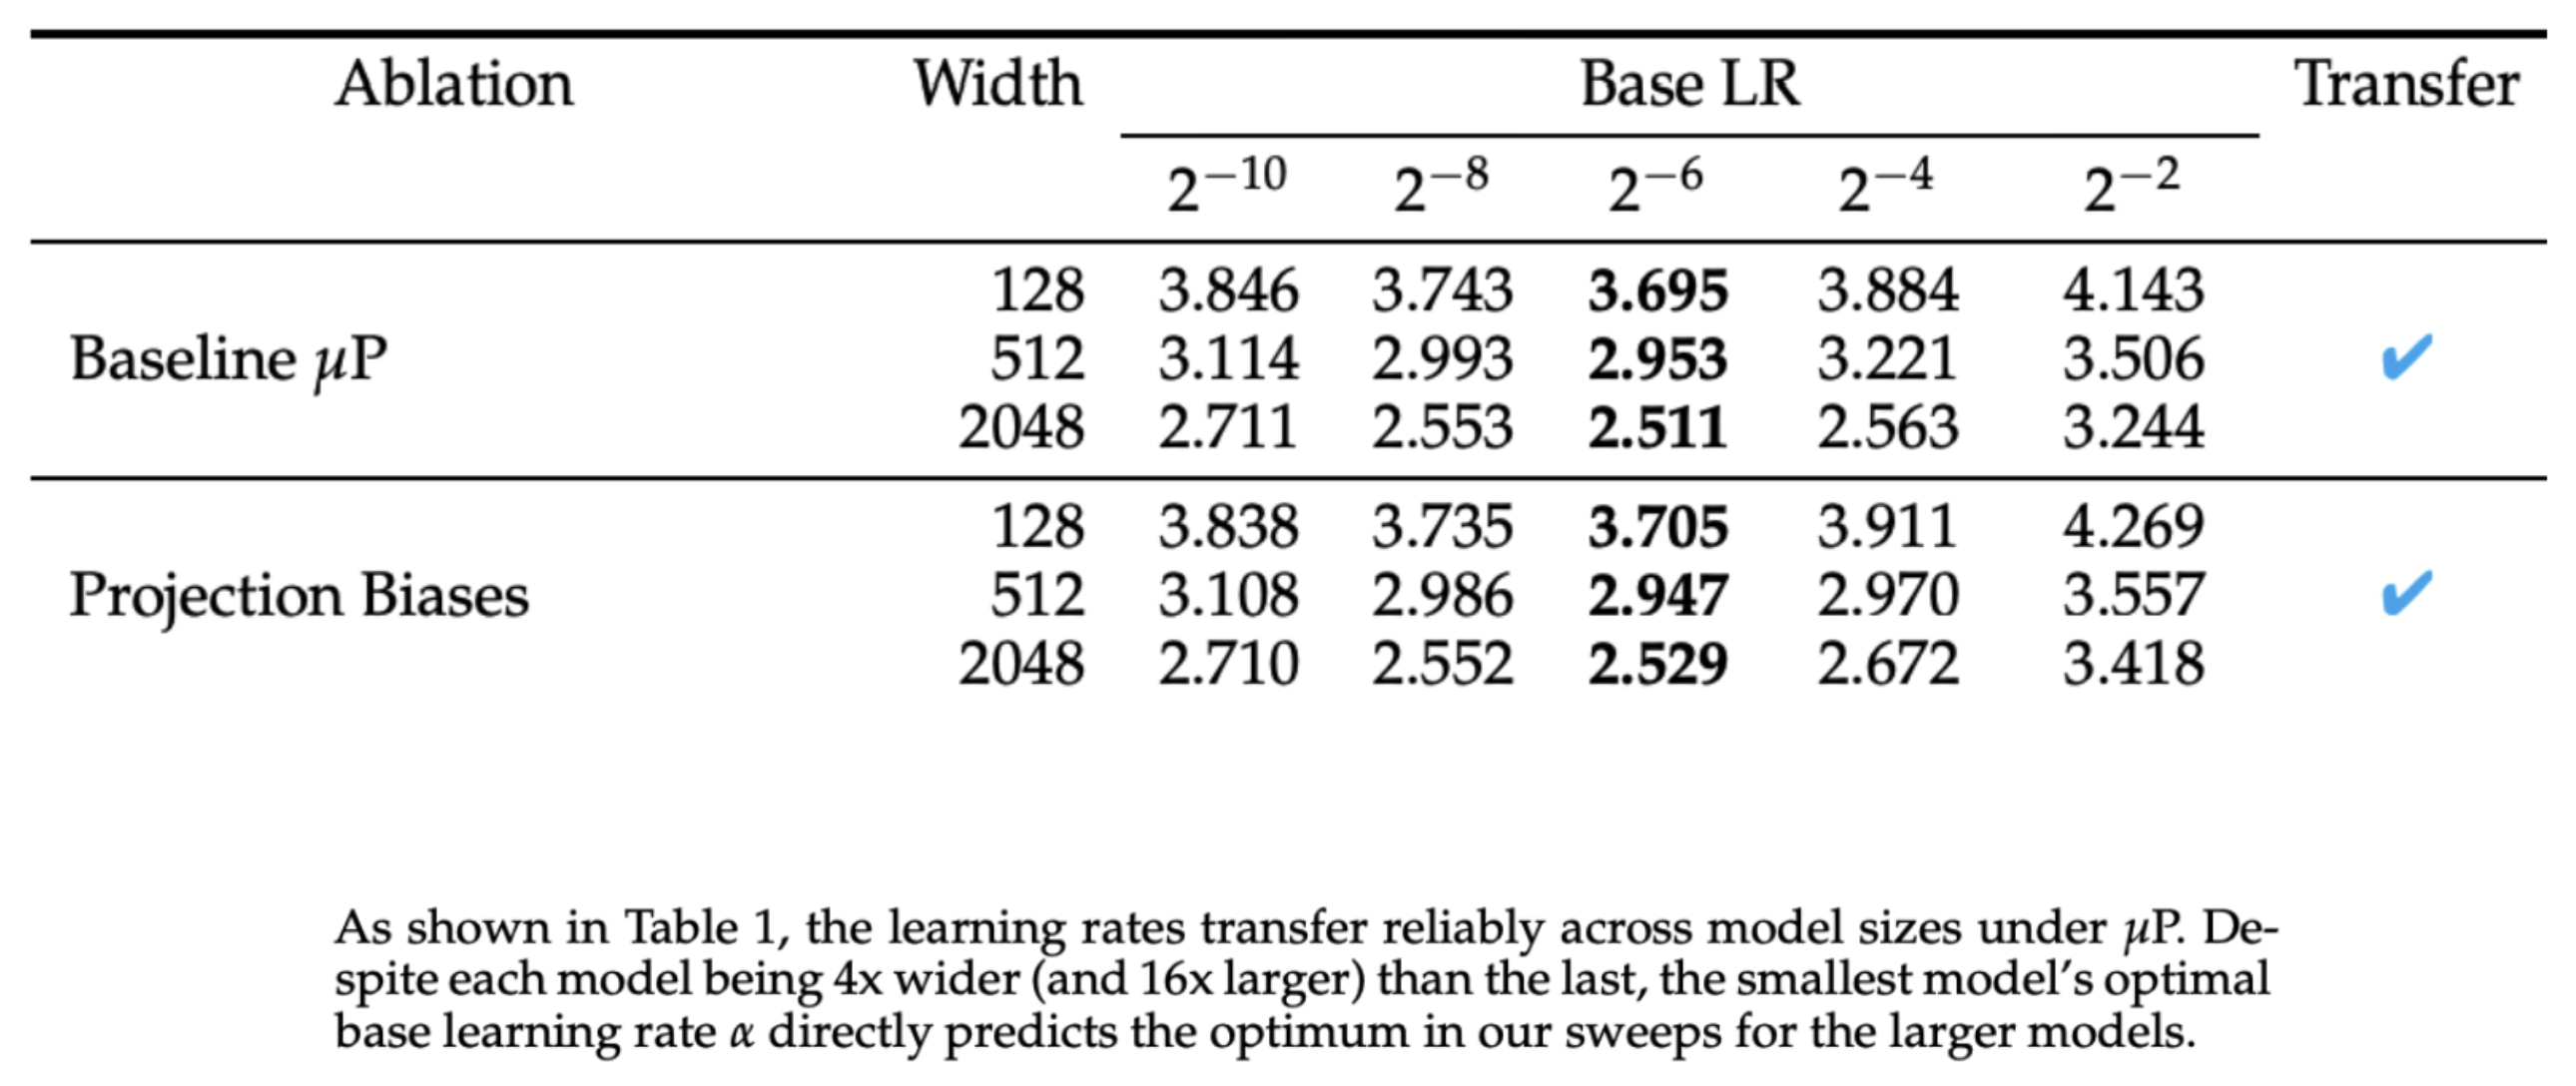
\includegraphics[width=1\linewidth]{replicating.png}
\end{figure}

\subsection*{What is muP robust to?}

Modern LMs have many components that deviate from muP's theory.

\begin{itemize}
    \item Activations - SwiGLU and squared ReLU
    \item Batch sizes - Large / small
    \item Initialization variations - zero attention, etc.
    \item RMSNorm gains
    \item Exotic optimizers (Lion)
    \item Regularizers
\end{itemize}

Which of these (if any) break muP?

\subsubsection*{What is muP not robust to? RMSNorm gain}

In our arch - RMSNorm has learnable gains. This turns out to break muP.

\begin{figure}[hpbt]
    \centering
    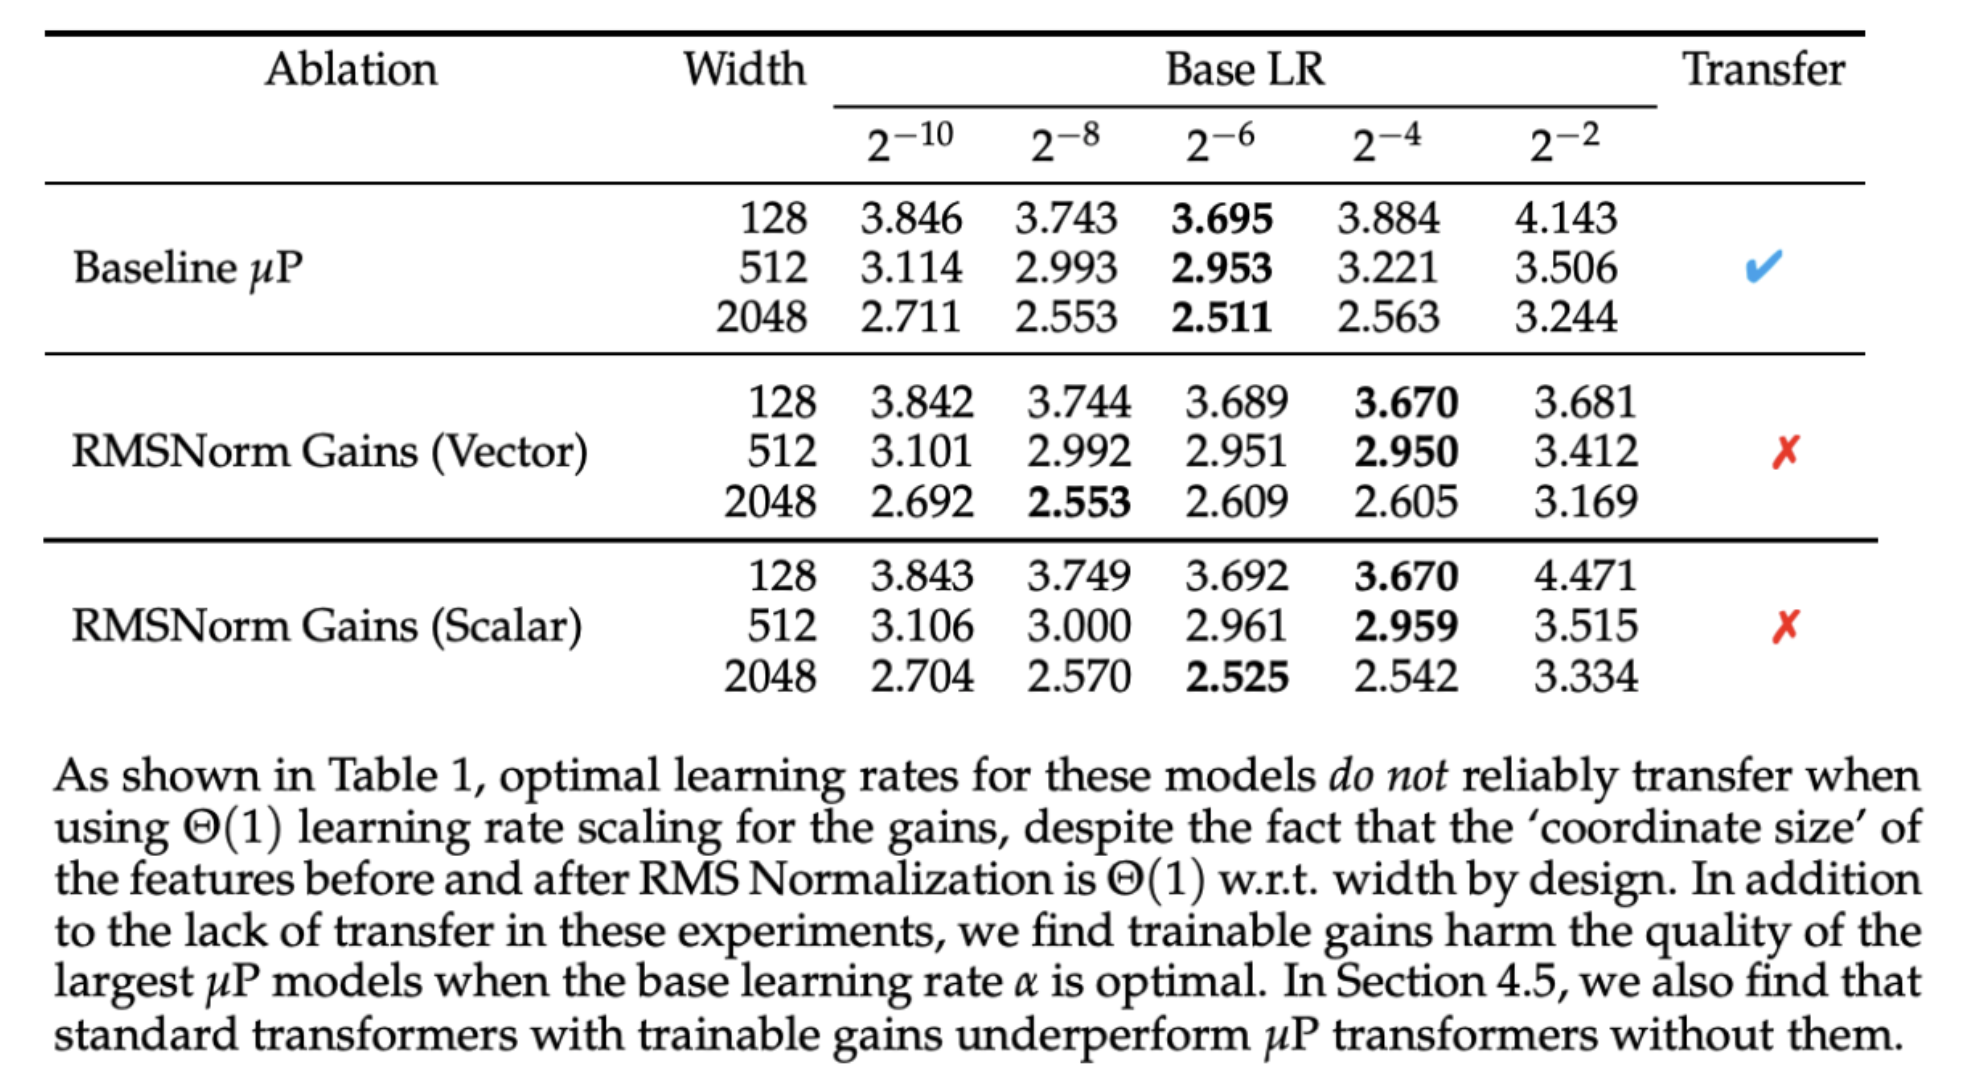
\includegraphics[width=1\linewidth]{rmsnorm.png}
\end{figure}

But these gains can be removed with little loss of performance\ldots

\subsubsection*{What is muP not robust to? Exotic optimizers}

There are other, exotic optimizers based on just gradient signs. Do they transfer?

\begin{figure}[H]
    \centering
    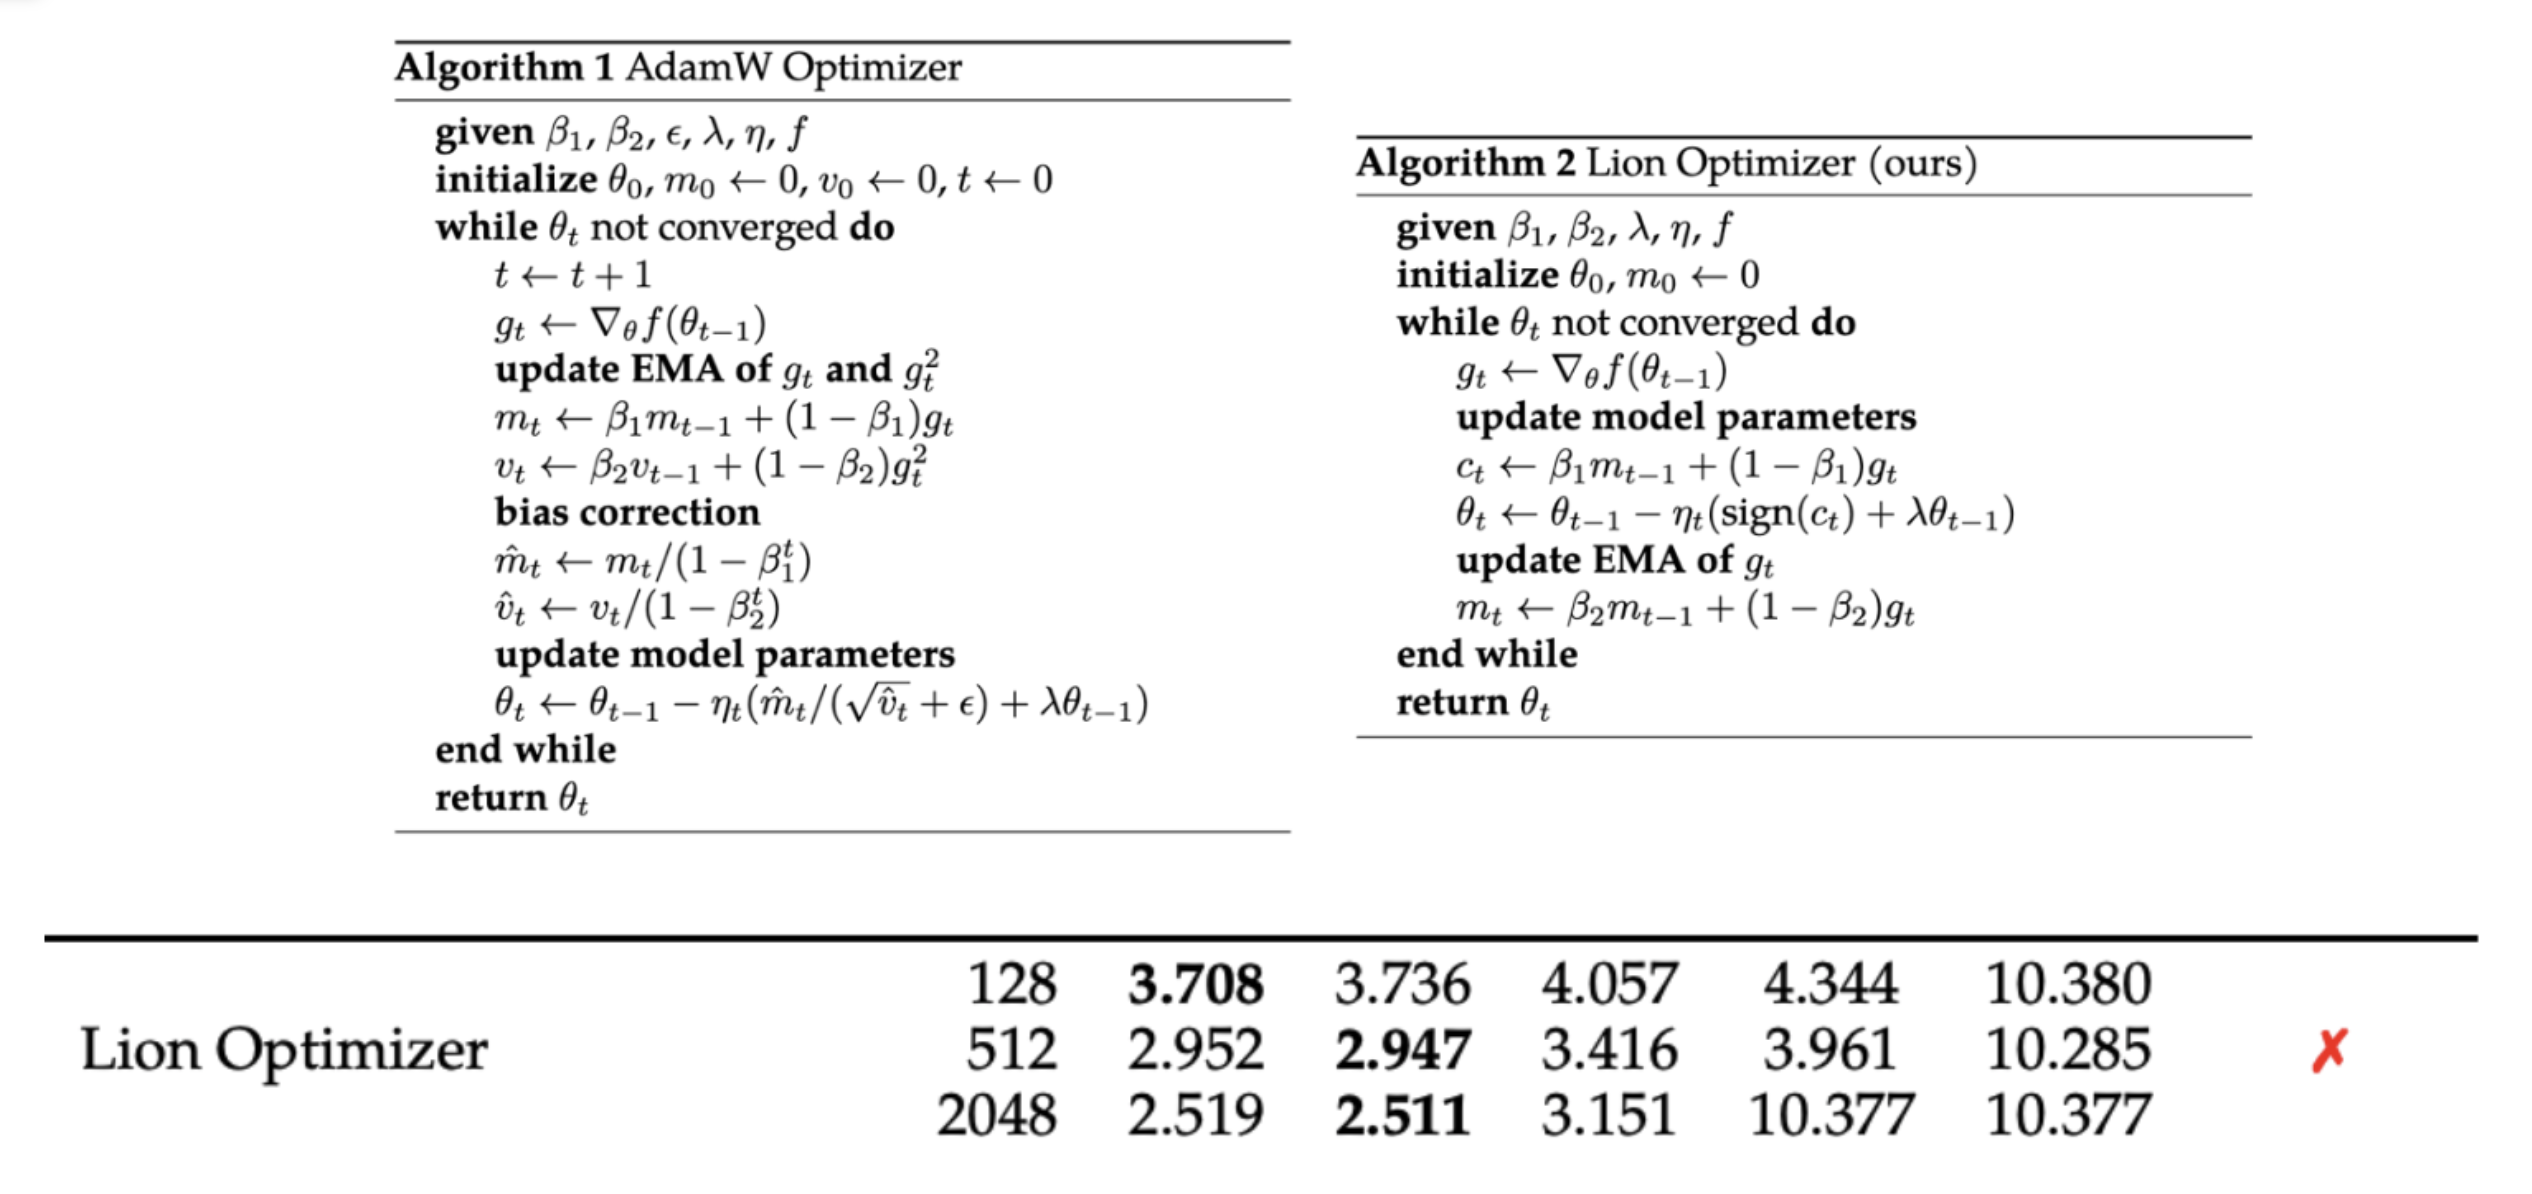
\includegraphics[width=1\linewidth]{algorithm.png}
\end{figure}

\subsubsection*{What is muP not robust to? (strong) weight decay}

What about strong (0.1) weight decay? This is maybe the only significant muP failure!

\begin{figure}[hpbt]
    \centering
    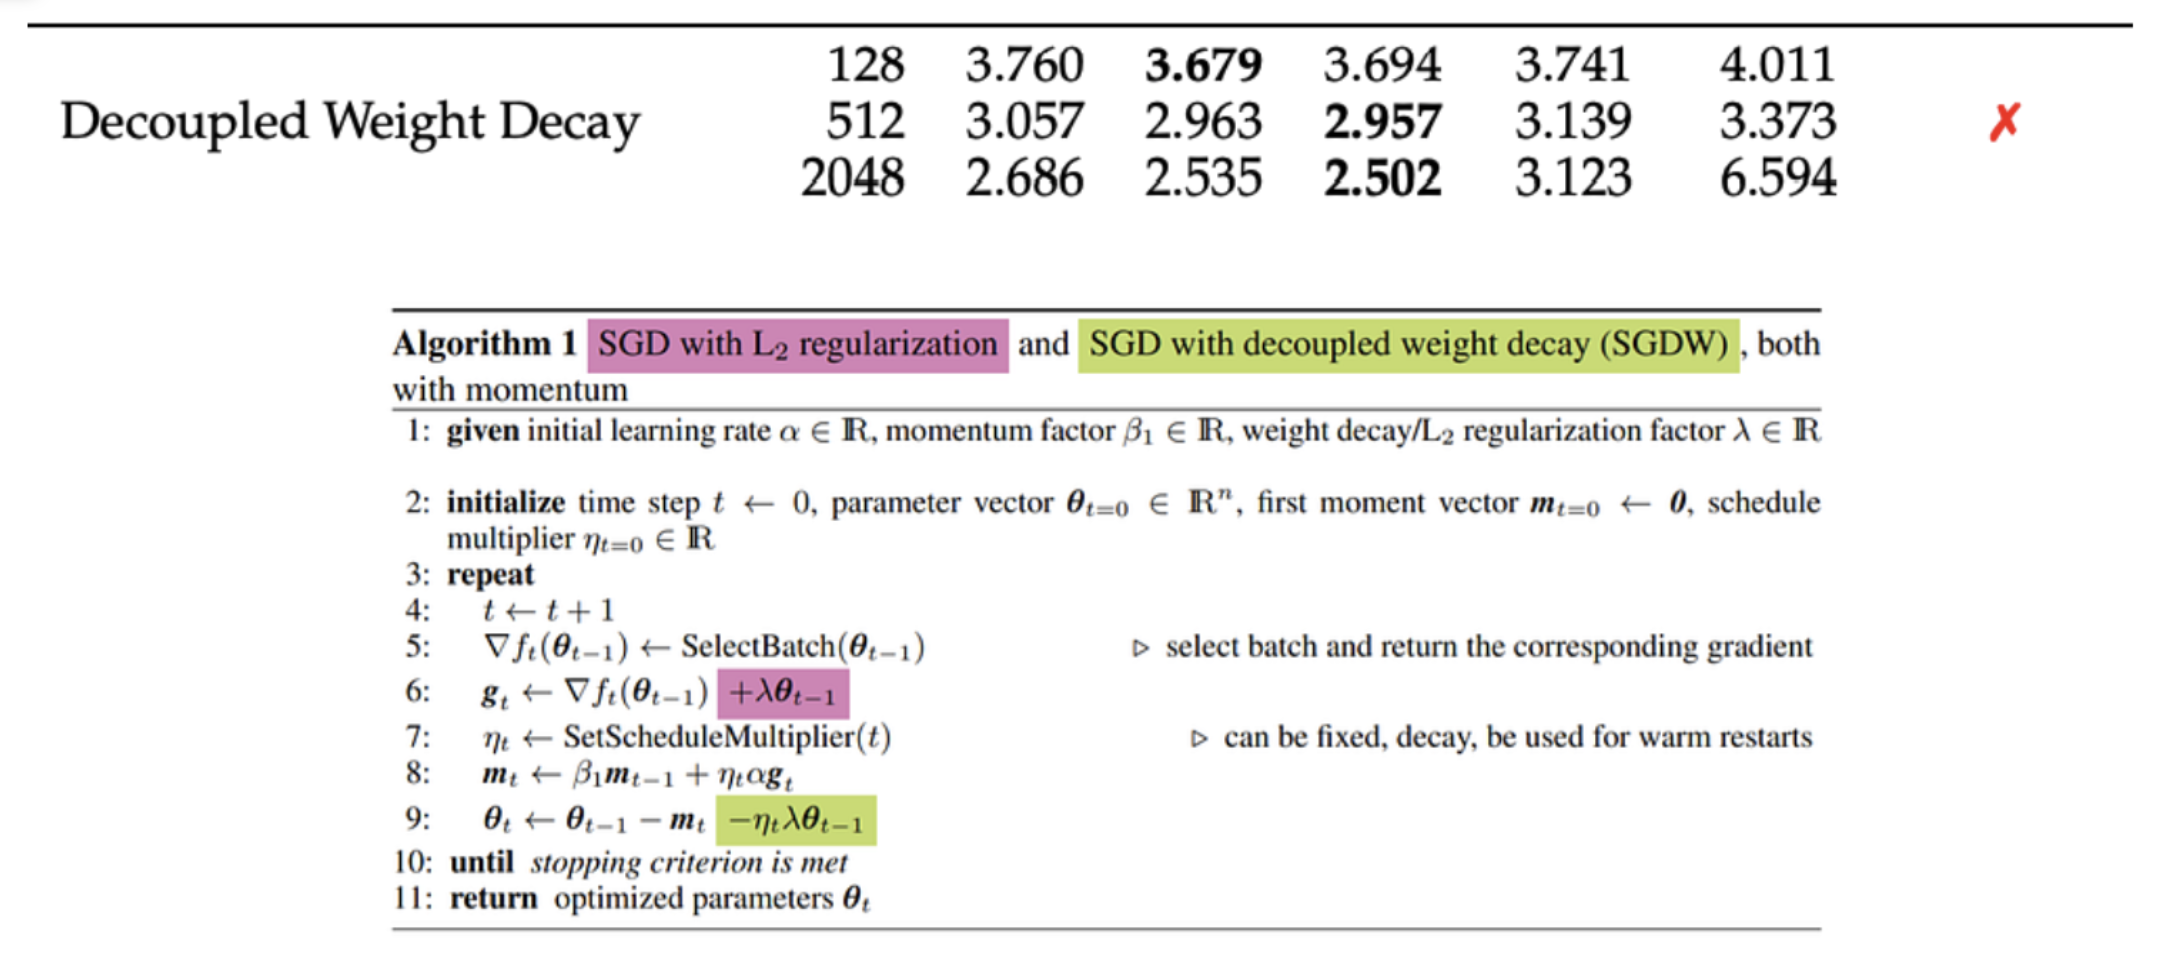
\includegraphics[width=1\linewidth]{robust.png}
\end{figure}

\subsubsection*{Is muP useful? At least to some extent\ldots}

\begin{enumerate}
    \item Overall, muP generally seems useful - insofar as SP is quite a bit more unstable.
    \item Current evidence suggests that muP parameterization / initialization may be easier to tune.
\end{enumerate}
\end{document}
